\pdfoutput=1
\documentclass[11pt]{article}
\usepackage[preprint]{acl}
\usepackage{times}
\usepackage{latexsym}
\usepackage[T1]{fontenc}
\usepackage[utf8]{inputenc}
\usepackage{microtype}
\usepackage{inconsolata}
\usepackage{graphicx}
\usepackage{booktabs}
\usepackage{multirow}
\usepackage{amsmath}
\usepackage{amssymb}
\usepackage{amsthm}
\usepackage{mathtools}
\usepackage{enumitem}
\usepackage{tikz}
\usetikzlibrary{arrows.meta,positioning,shapes.geometric,fit,backgrounds}

\setcounter{topnumber}{4}
\setcounter{bottomnumber}{4}
\setcounter{totalnumber}{8}
\setcounter{dbltopnumber}{4}
\renewcommand{\topfraction}{0.95}
\renewcommand{\bottomfraction}{0.95}
\renewcommand{\textfraction}{0.05}
\renewcommand{\floatpagefraction}{0.85}
\renewcommand{\dbltopfraction}{0.95}
\renewcommand{\dblfloatpagefraction}{0.85}

\newtheorem{theorem}{Theorem}
\newtheorem{proposition}{Proposition}
\newtheorem{lemma}{Lemma}
\newtheorem{definition}{Definition}

\title{\textbf{U-GraphRAG}: Reliable Retrieval-Augmented Generation via Uncertainty-Routed Graph Selection and Calibrated Decoding}

\author{
  \textbf{Zhou Xing} \quad \textbf{Song Li} \\
  School of Computing and Artificial Intelligence \\
  Shandong University of Finance and Economics \\
  \texttt{zhouxing@sdufe.edu.cn}, \texttt{LindaSong@gmail.com}
}

\begin{document}
\maketitle

\begin{abstract}
Retrieval-Augmented Generation (RAG) systems deployed over noisy, multi-hop, and conflicting corpora face three coupled bottlenecks: (1) retrieving a fixed top-$K$ passage set wastes $50\%\text{--}80\%$ of context tokens on simple queries, whereas uncalibrated entropy thresholds trigger erroneous early-exits on homogeneous off-topic pools; (2) diversity rerankers such as Maximal Marginal Relevance (MMR) retain $>95\%$ of injected contradictions, while un-gated probability-divergence penalties suppress complementary multi-hop bridge passages; and (3) contrastive decoding improves context adherence by subtracting the parametric prior, yet computing answer confidence from contrastively sharpened logits produces poorly calibrated probabilities.

We propose \textbf{U-GraphRAG}, a training-free, single-GPU RAG framework coordinating three stages: \textbf{M1} estimates epistemic uncertainty from first-token entropy using model-specific development quantiles, blocks off-topic or conflicting early-exits via relevance and shingle-overlap guards, and expands remaining queries over a Bloom-pruned MinHash LSH entity graph; \textbf{M2} selects a size-constrained evidence subset with an overlap-gated Jensen-Shannon conflict penalty and orders passages via a Kruskal Maximum Spanning Forest traversal; and \textbf{M3} separates contrastive answer generation ($\beta=0.12$) from unmodulated probability extraction ($\beta=0$), followed by Platt scaling and finite-sample Split Conformal abstention. Across \textbf{97,240 test evaluations} covering \textbf{324 multi-seed runs} ($71,280$ evaluations across 3 backbones $\times$ 4 QA tasks $\times$ 9 ablations), \textbf{7,920 6-axis stress evaluations}, \textbf{2,080 zero-tuning OOD transfer evaluations}, and a \textbf{15,960-run comparison} against \texttt{BGE-Reranker-Large}, \texttt{CK-PLUG} (ICLR'26), \texttt{InstructRAG-ICL} (ICLR'25), and \texttt{CAD} (NAACL'24), U-GraphRAG obtains the highest 12-block macro-average F1 (\textbf{52.05\%}, Friedman $p = 1.37 \times 10^{-10}$), reduces macro-average ECE by \textbf{78.8\%} (\textbf{0.0720} vs.\ 0.3404, Friedman $p = 9.90 \times 10^{-6}$), ranks first across all three backbones on counterfactual \texttt{NQ-Swap Dual} (\textbf{+7.32 to +28.56 pp} over the strongest baseline), reaches \textbf{69.40\% Raw F1 / 75.58\% Selective Acc} on mixed-conflict \texttt{RAMDocs} (\texttt{Qwen2.5-7B}), reduces \texttt{HotpotQA} conflict retention from \textbf{72.5\%--100\% to 9.17\%--10.00\%}, and eliminates erroneous off-topic early-exits in Scenario S4 (\textbf{85.83\%} down to \textbf{0.0\%}) under single-GPU 4-bit NF4 constraints.
\end{abstract}

\section{Introduction}

Retrieval-Augmented Generation (RAG) mitigates the parametric staleness and hallucination tendencies of Large Language Models (LLMs) by conditioning generation on external evidence passages retrieved from a large corpus \cite{yang2018hotpotqa,mallen2023popqa}. Despite rapid progress across conflict-aware RAG \cite{wei2025instructrag,xiang2024robustrag,wang2025madamrag,bi2026ckplug}, uncertainty-driven adaptive retrieval \cite{su2024dragin,jeong2024adaptiverag,yao2025seakr,adarague2025}, and contrastive or conformal decoding \cite{shi2024cad,gema2025decore,sinha2025crg}, deploying reliable RAG systems under strict single-GPU memory and latency constraints exposes three unresolved methodological tensions:

\begin{enumerate}[leftmargin=*,nosep]
    \item \textbf{Cross-Backbone Entropy Scale Drift and Ungrounded Early-Exit (Module M1)}: Token-level predictive entropy differs substantially across LLM families (the 60th-percentile epistemic estimate on \texttt{HotpotQA} Dev is $0.2015$ for \texttt{Qwen2.5-3B}, $0.0749$ for \texttt{Qwen2.5-7B}, and $0.6281$ for \texttt{Llama-3.1-8B}). Fixed scalar routing cutoffs do not transfer across backbones. Moreover, when the initial passages $\mathcal{D}_0$ are topically uniform yet off-topic (Scenario S4) or contain an unflagged contradiction, next-token entropy can remain artificially low and trigger an erroneous early-exit.
    \item \textbf{Preserving Complementary Multi-Hop Bridges While Filtering Contradictions (Module M2)}: In multi-hop reasoning (\texttt{HotpotQA}, \texttt{2WikiMultiHopQA}, \texttt{MuSiQue}), a first-hop bridge passage $d_1$ (e.g., naming a film's director) and a second-hop answer passage $d_2$ (stating the director's birthplace) naturally produce divergent single-passage answer distributions ($D_{\text{JS}}(P_1 \parallel P_2) \gg 0$). Un-gated divergence penalties suppress such complementary bridge pairs---reducing clean \texttt{HotpotQA} F1 from $46.63\%$ to $22.64\%$ as conflict weight $\lambda_4$ increases from $1.0$ to $10.0$---whereas surface diversity methods such as MMR \cite{carbonell1998mmr} retain $96.25\%$ of injected contradicting passages.
    \item \textbf{Conflict Between Contrastive Decoding and Probability Calibration (Module M3)}: Contrastive decoding methods such as CAD \cite{shi2024cad} and CK-PLUG \cite{bi2026ckplug} strengthen context reliance via $(1+\beta)\mathbf{z}_t^{\text{ctx}} - \beta\mathbf{z}_t^{\text{prior}}$. Yet extracting confidence scores from contrastively shifted and truncated logits concentrates probability mass onto the top token, impairing confidence discrimination (AUROC $0.5267$ on \texttt{HotpotQA}) and raising false abstention rates ($43.75\%$).
\end{enumerate}

In this paper, we present a systematic theoretical and empirical study of \textbf{U-GraphRAG}, a resource-bounded selective RAG framework evaluated under noisy, conflicting, and off-topic retrieval across multi-seed cross-family benchmarks, 6-axis controlled perturbations, zero-tuning cross-dataset transfer, post-hoc Split Conformal Risk Control, and controlled comparisons against recent training-free baselines (\texttt{BGE-Reranker}, \texttt{CK-PLUG}, \texttt{InstructRAG-ICL}, and \texttt{CAD}). Reproduction scripts and evaluation logs will be released publicly upon competition and review completion.

\section{Related Work and Grounded Literature Positioning}

A systematic audit of 2024--2026 top-venue RAG literature reveals three distinct evolutionary tracks:

\paragraph{Track A: Conflict Resolution and Robust RAG.}
\textbf{InstructRAG} \cite{wei2025instructrag} synthesizes explicit denoising rationales ($r$) to filter noisy passages via instruction tuning (FT) or training-free in-context learning (ICL), though its strongest FT mode requires per-dataset multi-GPU fine-tuning. \textbf{RobustRAG} \cite{xiang2024robustrag} adopts an \emph{Isolate-then-Aggregate} architecture with keyword or decoding aggregation for certifiable corruption resistance, incurring $1.16\text{--}3.65\times$ latency overhead and degrading when corrupted sources form a majority. \textbf{MADAM-RAG} \cite{wang2025madamrag} assigns an independent LLM agent per document for multi-round debate, achieving $57.70\%$ EM on FaithEval and $34.40\%$ EM on the mixed-conflict RAMDocs benchmark, but consumes $29.44\text{ GB}$ VRAM on \texttt{Qwen2.5-7B} (exceeding a single 24 GB RTX 4090). \textbf{CK-PLUG} \cite{bi2026ckplug} detects token-level parametric-vs.-context conflict via negative Confidence Gain ($\text{IG} = H_{\text{prior}} - H_{\text{ctx}} < |H_{\text{ctx}}|$) and modulates logits without training, yet leaves the post-modulation probability distribution uncalibrated for downstream selective abstention. Other recent works explore internal-external reconciliation (\textbf{Astute RAG}, \citealp{wang2025astuterag}), reinforcement learning under counterfactual contexts (\textbf{Knowledgeable-R1}, \citealp{knowledgeabler1_2026}), and NLI maximum independent sets (\textbf{ReliabilityRAG}, \citealp{reliabilityrag2025}).

\paragraph{Track B: Uncertainty-Driven and Self-Aware Adaptive Retrieval.}
\textbf{DRAGIN} \cite{su2024dragin} monitors token entropy and attention during generation to trigger mid-sentence queries, while \textbf{Adaptive-RAG} \cite{jeong2024adaptiverag} trains a complexity classifier to route queries across 0/1/multi-step retrieval. \textbf{SEAKR} \cite{yao2025seakr} extracts self-aware uncertainty from the regularized Gram determinant of hidden states, and \textbf{Internal Confidence} \cite{chen2026internalconfidence} aggregates pre-generation hidden states across decision-center layers. \textbf{Self-RAG} \cite{asai2024selfrag} and \textbf{CRAG} \cite{yan2024crag} rely on fine-tuned reflection tokens or an external $0.77\text{B}$ evaluator. Crucially, the ACL 2025 benchmark \textbf{AdaRAGUE} \cite{adarague2025} reproduced Adaptive-RAG, DRAGIN, FLARE, and SEAKR across six datasets (500 samples each), proving that lightweight uncertainty proxies match complex internal self-knowledge probes in routing efficacy---motivating U-GraphRAG's lightweight entropy routing estimator while highlighting the necessity of explicit relevance guards on off-topic candidate pools.

\paragraph{Track C: Contrastive Decoding, Calibration, and Conformal Risk Control.}
\textbf{CAD} \cite{shi2024cad}, \textbf{DoLa} \cite{chuang2024dola}, and \textbf{DeCoRe} \cite{gema2025decore} contrast context-conditioned or retrieval-head-masked logits to suppress hallucinations ($40.74\%$ EM on PopQA for $\text{DeCoRe}_{\text{static}}$). On the risk-control front, \textbf{Conformal RAG Guardrails (CRG)} \cite{sinha2025crg} exposed the \emph{Semantic Illusion}: uncertainty detectors achieving $0.81\text{--}0.83$ AUROC and $0\%$ FPR on synthetic benchmarks degrade to $100\%$ FPR on real HaluEval under a $95\%$ recall constraint (and drop from $95\%$ to $11\%$ coverage under $\text{NQ}\to\text{RAGTruth}$ shift). Recent frameworks (\textbf{CoFact}, \citealp{cofact2026}; \textbf{DualStake}, \citealp{dualstake2026}) target conformal factuality calibration and selective AURC reduction. U-GraphRAG connects Tracks A, B, and C within one training-free pipeline combining overlap-gated subset selection, graph ordering, unmodulated probability scaling, and Split Conformal Risk Control.

\section{Methodology: Foundational Preliminaries and U-GraphRAG Architecture}

To make the algorithmic pipeline self-contained, we first review the foundational neural, retrieval, information-theoretic, graph-theoretic, and statistical calibration primitives that underlie U-GraphRAG, specifying their originators, core mechanisms, and exact roles prior to formalizing Modules M1--M3.

\subsection{Foundational Preliminaries and System Overview}
\label{sec:preliminaries}

\paragraph{Autoregressive Transformer Backbones and 4-Bit Quantization.}
All generators evaluated in this work belong to the decoder-only \textbf{Transformer} family introduced by \citet{vaswani2017attention}. Unlike recurrent neural networks that process tokens sequentially, the Transformer models arbitrary-distance dependencies in parallel through scaled dot-product multi-head self-attention, interleaved with position-wise feed-forward layers and residual connections. In autoregressive causal language modeling, triangular causal masking ensures that at decoding step $t$, the logit vector $\mathbf{z}_t = \text{Logits}_{\theta}(y_t \mid q, \mathcal{E}, y_{<t}) \in \mathbb{R}^{|\mathcal{V}|}$ depends strictly on the query $q$, retrieved context $\mathcal{E}$, and previously generated tokens $y_{<t}$, inducing next-token probabilities $P_{\theta}(y_t \mid q, \mathcal{E}, y_{<t}) = \mathrm{Softmax}(\mathbf{z}_t)$. To fit 3B--8B Transformer weights within a single consumer GPU budget ($<24\text{ GB}$ VRAM) without parameter updates, we store frozen weights using \textbf{4-bit NormalFloat (NF4) quantization} proposed by \citet{dettmers2023qlora}. NF4 partitions weight quantization bins along quantiles of the standard normal distribution to minimize expected quantization distortion, reducing memory consumption by nearly $4\times$ relative to 16-bit weights.

\paragraph{Sparse, Dense, and Rank-Fused Retrieval Primitives.}
Given a query $q \in \mathcal{Q}$ and corpus $\mathcal{C} = \{d_1, \dots, d_M\}$, first-stage retrieval balances exact lexical matching against semantic paraphrase sensitivity:
\begin{itemize}[leftmargin=*,nosep]
    \item \textbf{BM25} \cite{robertson2009bm25}: A probabilistic sparse retrieval scoring model developed by Robertson and Zaragoza that combines inverse document frequency with saturating term-frequency normalization and document-length scaling to retrieve exact named entities and rare terms reliably.
    \item \textbf{Dense Bi-Encoder Retrieval} \cite{karpukhin2020dpr}: Introduced for open-domain QA by Karpukhin et al., bi-encoders map queries and passages independently into a dense vector space (\texttt{BAAI/bge-small-en-v1.5}, \citealp{chen2024bgem3}) so semantic proximity can be scored via inner-product similarity even without lexical overlap.
    \item \textbf{Reciprocal Rank Fusion (RRF)} \cite{cormack2009rrf}: Proposed by Cormack et al., RRF merges heterogeneous rankings without score calibration via $\text{RRF}(d) = \sum_{r} (k + \text{rank}_r(d))^{-1}$ ($k=60$). Using $\text{RRF}_{k=60}$ over BM25 and dense rankings produces an initial seed set $\mathcal{D}_0 = (d_1, \dots, d_{k_0})$ ($k_0 = 3$) inside a candidate pool $\mathcal{D}_{\text{pool}}$ ($|\mathcal{D}_{\text{pool}}| \le 16$).
    \item \textbf{Maximal Marginal Relevance (MMR)} \cite{carbonell1998mmr}: Proposed by Carbonell and Goldstein, MMR selects candidates iteratively by balancing query relevance against maximum similarity to already selected passages. While effective for eliminating surface redundancy, MMR cannot distinguish paraphrased conflict from helpful variety, motivating Module M2.
\end{itemize}

\begin{figure*}[t]
\centering
\resizebox{\textwidth}{!}{
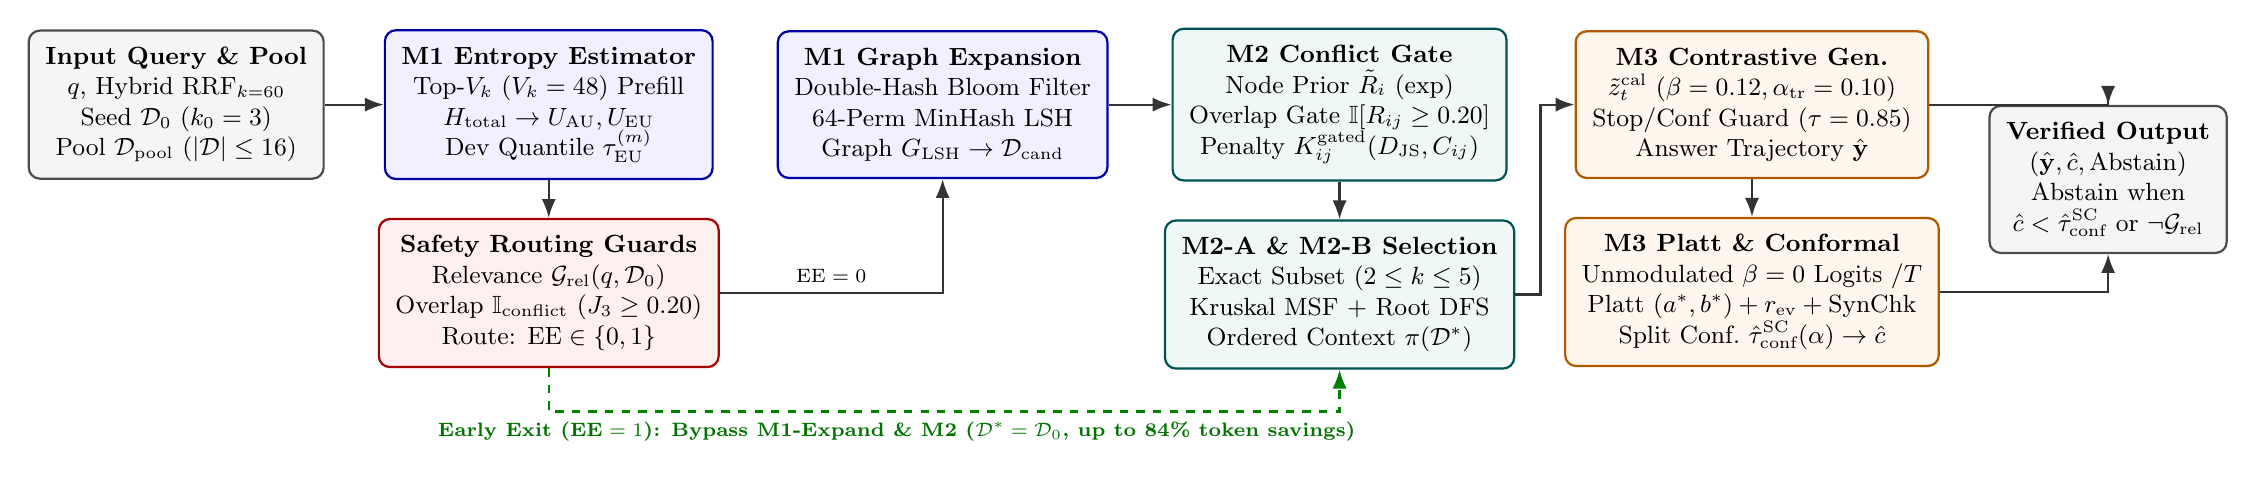
\begin{tikzpicture}[
    node distance=0.55cm and 0.85cm,
    box/.style={rectangle, rounded corners=4pt, draw=black!70, thick, align=center, font=\small, inner sep=6pt, fill=white},
    m1box/.style={box, fill=blue!6, draw=blue!65!black},
    m2box/.style={box, fill=teal!6, draw=teal!65!black},
    m3box/.style={box, fill=orange!7, draw=orange!70!black},
    gatebox/.style={box, fill=red!6, draw=red!65!black},
    arr/.style={-{Latex[length=2.4mm]}, thick, draw=black!80},
    dasharr/.style={-{Latex[length=2.4mm]}, thick, dashed, draw=green!50!black}
]
% Stage 0: Input & RRF Retrieval
\node[box, fill=gray!8] (inp) {\textbf{Input Query \& Pool}\\$q$, Hybrid $\text{RRF}_{k=60}$\\Seed $\mathcal{D}_0$ ($k_0=3$)\\Pool $\mathcal{D}_{\text{pool}}$ ($|\mathcal{D}|\le 16$)};

% Stage 1: Module M1
\node[m1box, right=0.75cm of inp] (m1p) {\textbf{M1 Entropy Estimator}\\Top-$V_k$ ($V_k=48$) Prefill\\$H_{\text{total}} \to U_{\text{AU}}, U_{\text{EU}}$\\Dev Quantile $\tau_{\text{EU}}^{(m)}$};
\node[gatebox, below=0.48cm of m1p] (m1g) {\textbf{Safety Routing Guards}\\Relevance $\mathcal{G}_{\text{rel}}(q, \mathcal{D}_0)$\\Overlap $\mathbb{I}_{\text{conflict}}$ ($J_3\ge 0.20$)\\Route: $\text{EE} \in \{0,1\}$};
\node[m1box, right=0.80cm of m1p] (m1e) {\textbf{M1 Graph Expansion}\\Double-Hash Bloom Filter\\64-Perm MinHash LSH\\Graph $G_{\text{LSH}} \to \mathcal{D}_{\text{cand}}$};

% Stage 2: Module M2
\node[m2box, right=0.80cm of m1e] (m2g) {\textbf{M2 Conflict Gate}\\Node Prior $\tilde{R}_i$ ($\text{exp}$)\\Overlap Gate $\mathbb{I}[R_{ij}\ge 0.20]$\\Penalty $K_{ij}^{\text{gated}}(D_{\text{JS}}, C_{ij})$};
\node[m2box, below=0.48cm of m2g] (m2o) {\textbf{M2-A \& M2-B Selection}\\Exact Subset ($2\le k\le 5$)\\Kruskal MSF + Root DFS\\Ordered Context $\pi(\mathcal{D}^*)$};

% Stage 3: Module M3
\node[m3box, right=0.85cm of m2g] (m3d) {\textbf{M3 Contrastive Gen.}\\$\tilde{z}_t^{\text{cal}}$ ($\beta=0.12, \alpha_{\text{tr}}=0.10$)\\Stop/Conf Guard ($\tau=0.85$)\\Answer Trajectory $\hat{\mathbf{y}}$};
\node[m3box, below=0.48cm of m3d] (m3c) {\textbf{M3 Platt \& Conformal}\\Unmodulated $\beta=0$ Logits $/ T$\\Platt $(a^*, b^*) + r_{\text{ev}} + \text{SynChk}$\\Split Conf.\ $\hat{\tau}_{\text{conf}}^{\text{SC}}(\alpha) \to \hat{c}$};

% Output
\node[box, fill=gray!8, right=0.75cm of m3d, yshift=-0.95cm] (out) {\textbf{Verified Output}\\$(\hat{\mathbf{y}}, \hat{c}, \text{Abstain})$\\Abstain when\\$\hat{c} < \hat{\tau}_{\text{conf}}^{\text{SC}}$ or $\neg \mathcal{G}_{\text{rel}}$};

% Edges
\draw[arr] (inp) -- (m1p);
\draw[arr] (m1p) -- (m1g);
\draw[arr] (m1g.east) -| node[pos=0.25, above, font=\scriptsize] {$\text{EE}=0$} (m1e.south);
\draw[arr] (m1e) -- (m2g);
\draw[arr] (m2g) -- (m2o);
\draw[arr] (m2o.east) -- ++(0.32,0) |- (m3d.west);
\draw[arr] (m3d) -- (m3c);
\draw[arr] (m3d.east) -| (out.north);
\draw[arr] (m3c.east) -| (out.south);

% Fast Path Early Exit
\draw[dasharr] (m1g.south) -- ++(0,-0.55) -| node[pos=0.22, below, font=\scriptsize\bfseries, text=green!45!black] {Early Exit ($\text{EE}=1$): Bypass M1-Expand \& M2 ($\mathcal{D}^*=\mathcal{D}_0$, up to 84\% token savings)} (m2o.south);
\end{tikzpicture}
}
\caption{End-to-End Architecture of \textbf{U-GraphRAG}. Module M1 estimates epistemic uncertainty under relevance and overlap safety guards ($\mathcal{G}_{\text{rel}}$ and $\mathbb{I}_{\text{conflict}}$), expanding non-exiting queries via Bloom filtering and MinHash LSH into Module M2's overlap-gated subset selector and spanning-forest ordering. Module M3 separates contrastive answer generation ($\beta=0.12$) from unmodulated probability calibration (\texttt{calib\_from\_b0}), Platt scaling, and Split Conformal Risk Control.}
\label{fig:arch}
\end{figure*}

Under this frozen 4-bit causal Transformer $P_{\theta}(y \mid q, \mathcal{E})$, U-GraphRAG maps $(q, \mathcal{D}_{\text{pool}})$ to $(\hat{\mathbf{y}}, \hat{c}, \text{Abstain}) \in \mathcal{V}^* \times [0, 1] \times \{0, 1\}$ through the three-stage pipeline summarized in Figure~\ref{fig:arch}.

\subsection{Module M1: Uncertainty-Routed Adaptive Retrieval and Graph Expansion}

\subsubsection{Entropy Estimation and Uncertainty Decomposition}
\paragraph{Background: Shannon Entropy and Uncertainty Types.}
Introduced by \citet{shannon1948mathematical}, \textbf{Shannon entropy} $H(P) = -\sum_v p(v)\ln p(v)$ quantifies the average surprise or dispersion of a discrete probability distribution and equals zero when all mass lies on a single outcome. In machine learning, \citet{hullermeier2021aleatoric} distinguish two components of predictive uncertainty: \textbf{aleatoric uncertainty} (irreducible noise or surface ambiguity inherent in the phrasing of inputs) and \textbf{epistemic uncertainty} (knowledge deficiency arising from missing evidence or unresolved model ignorance that additional retrieval can reduce). To avoid costly multi-sample Bayesian approximations during single-GPU inference, M1 computes a lightweight decomposition in a single prefill pass (\texttt{use\_cache=False, logits\_to\_keep=1}) over the top-$V_k$ ($V_k = 48$) vocabulary support $\mathcal{V}_k \subset \mathcal{V}$:
\begin{align}
H_{\text{total}}(q, \mathcal{D}_0) &= -\sum_{v \in \mathcal{V}_k} \tilde{p}(v \mid q, \mathcal{D}_0) \nonumber \\
&\qquad \cdot \ln \tilde{p}(v \mid q, \mathcal{D}_0), \label{eq:m1_htotal} \\
\tilde{p}(v \mid q, \mathcal{D}_0) &= \frac{P_{\theta}(v \mid q, \mathcal{D}_0)}{\sum_{w \in \mathcal{V}_k} P_{\theta}(w \mid q, \mathcal{D}_0)}. \nonumber
\end{align}
Let $\mathcal{W}(d_i)$ denote the normalized lexical word set of passage $d_i \in \mathcal{D}_0$. We capture surface lexical diversity within the initial seeds via mean pairwise Jaccard similarity $\bar{J}(\mathcal{D}_0)$ and lexical divergence $D_{\text{lex}}(\mathcal{D}_0) = 1 - \bar{J}(\mathcal{D}_0)$:
\begin{equation}
\bar{J}(\mathcal{D}_0) = \frac{2}{|\mathcal{D}_0|(|\mathcal{D}_0|-1)} \sum_{i < j} \frac{|\mathcal{W}(d_i) \cap \mathcal{W}(d_j)|}{|\mathcal{W}(d_i) \cup \mathcal{W}(d_j)|}.
\label{eq:m1_jbar}
\end{equation}
The surface-ambiguity proxy $U_{\text{AU}}$ and epistemic routing estimate $U_{\text{EU}}$ are decomposed algebraically as:
\begin{align}
U_{\text{AU}}(q, \mathcal{D}_0) &\triangleq \alpha_{\text{au}}\bigl(0.25 + 0.50 \, D_{\text{lex}}(\mathcal{D}_0)\bigr) \nonumber \\
&\quad \cdot H_{\text{total}}(q, \mathcal{D}_0), \label{eq:m1_uau} \\
U_{\text{EU}}(q, \mathcal{D}_0) &\triangleq \max\bigl(0, \, H_{\text{total}} - U_{\text{AU}}\bigr). \label{eq:m1_ueu}
\end{align}
With default $\alpha_{\text{au}} = 1.0$, Eq.~\eqref{eq:m1_ueu} reduces directly to $U_{\text{EU}}(q, \mathcal{D}_0) = (0.25 + 0.50 \, \bar{J}(\mathcal{D}_0)) H_{\text{total}}(q, \mathcal{D}_0) \ge 0$. For each expansion candidate $d_c \in \mathcal{D}_{\text{pool}} \setminus \mathcal{D}_0$, its marginal epistemic reduction is $\Delta U_{\text{EU}}(d_c \mid q, \mathcal{D}_0) = \max\bigl(0, U_{\text{EU}}(q, \mathcal{D}_0) - U_{\text{EU}}(q, \mathcal{D}_0 \cup \{d_c\})\bigr) \ge 0$.

\subsubsection{Backbone Quantile Calibration and Dual Safety Guards}
Because absolute logit temperatures and entropy ranges vary across pretrained backbones, we avoid test leakage and per-dataset tuning by fixing one model-level cutoff $\tau_{\text{EU}}^{(m)}$ per backbone at the 60th percentile ($q_{\text{target}} = 0.60$) of $N_{\text{dev}} = 80$ development queries from a single reference split (\texttt{HotpotQA} Dev):
\begin{align}
\tau_{\text{EU}}^{(m)} &\triangleq \text{Clip}_{[0.05, 0.90]}\Bigl( \mathcal{Q}_{\text{dev}}^{(m)} \Bigr), \label{eq:m1_anchor_tau} \\
\mathcal{Q}_{\text{dev}}^{(m)} &\triangleq \mathrm{Quant}_{0.60}\bigl(\{ U_{\text{EU}}^{(m)}(q_i, \mathcal{D}_{0,i}) \}_{i=1}^{N_{\text{dev}}}\bigr). \nonumber
\end{align}
This yields $\tau_{\text{EU}}^{\text{Qwen-3B}} = 0.2015$, $\tau_{\text{EU}}^{\text{Qwen-7B}} = 0.0749$, and $\tau_{\text{EU}}^{\text{Llama-8B}} = 0.6281$. To guard against erroneous early-exits when low entropy coincides with hidden contradiction or off-topic pools, M1 enforces two deterministic guards:
\begin{enumerate}[leftmargin=*,nosep]
    \item \textbf{Shingle-Overlap Conflict Guard ($\mathbb{I}_{\text{conflict}}$)}: Tests whether any pair in the top-5 pool shares 3-word shingle Jaccard overlap $J_{3\text{-sh}}(d_i, d_j) \ge \tau_{\text{sh}} = 0.20$, bypassing early-exit so M2 resolves potential claim contradictions:
    \begin{equation}
    \mathbb{I}_{\text{conflict}} \triangleq \mathbb{I}\Bigl[ \max_{1 \le i < j \le 5} J_{3\text{-sh}}(d_i, d_j) \ge \tau_{\text{sh}} \Bigr].
    \label{eq:m1_conflict_bypass}
    \end{equation}
    \item \textbf{Query-Evidence Relevance Floor Gate ($\mathcal{G}_{\text{rel}}$)}: Let $\rho_{\text{lex}}(q, d) = |\mathcal{W}_{\text{ctrl}}(q) \cap \mathcal{W}_{\text{ctrl}}(d)| / |\mathcal{W}_{\text{ctrl}}(q)|$ denote stopword-filtered content-word recall and $s(d)$ the first-stage retriever score. When homogeneous off-topic pools (Scenario S4) induce low entropy without answer support, $\mathcal{G}_{\text{rel}}$ blocks early-exit at zero extra GPU cost:
    \begin{align}
    \mathcal{G}_{\text{rel}}(q, \mathcal{D}_0) &\triangleq \mathbb{I}\Bigl[ \max_{d \in \mathcal{D}_0}\rho_{\text{lex}} \ge 0.45 \nonumber \\
    &\quad \lor \bigl(\max_{d \in \mathcal{D}_0}\rho_{\text{lex}} \ge 0.25 \nonumber \\
    &\qquad\quad \land \max_{d \in \mathcal{D}_0} s(d) \ge 0.70\bigr) \Bigr].
    \label{eq:m1_rel_gate}
    \end{align}
\end{enumerate}
Combining Eq.~\eqref{eq:m1_anchor_tau}--\eqref{eq:m1_rel_gate}, the routing decision $\text{EE} \in \{0,1\}$ is:
\begin{align}
\text{EE}(q, \mathcal{D}_{\text{pool}}) &\triangleq \mathbb{I}\bigl[U_{\text{EU}}(q, \mathcal{D}_0) \le \tau_{\text{EU}}^{(m)}\bigr] \nonumber \\
&\quad \cdot \mathcal{G}_{\text{rel}}(q, \mathcal{D}_0) \cdot (1 - \mathbb{I}_{\text{conflict}}).
\label{eq:m1_ee}
\end{align}

\subsubsection{Bloom Filtering and MinHash LSH Graph Expansion}
When $\text{EE}(q, \mathcal{D}_{\text{pool}}) = 0$, M1 filters and clusters remaining passages using two classic sub-linear data structures.

\paragraph{Bloom Filter and Kirsch-Mitzenmacher Double Hashing.}
Proposed by \citet{bloom1970space}, a \textbf{Bloom filter} is a compact $m$-bit bitset supporting $\mathcal{O}(1)$ set-membership testing with zero false negatives and bounded false-positive rate $p_{\text{fp}}$. Normally, setting $k$ bit indices requires evaluating $k$ independent hash functions per key. \citet{kirsch2006less} proved that generating $k$ indices via linear combinations of just two base hashes $h_1(x), h_2(x)$ preserves the exact asymptotic false-positive bound while reducing hashing cost to two evaluations per entity. M1 inserts query and seed entities $\mathcal{E}(q) \cup \mathcal{E}(\mathcal{D}_0)$ into this filter to prune disconnected passages:
\begin{equation}
h_r(x) = \left( h_1(x) + r \cdot h_2(x) \right) \bmod m,
\label{eq:m1_bloom}
\end{equation}
for $r \in \{0, \dots, k-1\}$, with optimal bit width $m = \lceil -n \ln p_{\text{err}} / (\ln 2)^2 \rceil$, hash count $k = \max(1, \text{round}((m/n)\ln 2))$, and theoretical false-positive rate $p_{\text{fp}} = (1 - e^{-kn/m})^k$.

\paragraph{MinHash Signatures and Locality-Sensitive Hashing (LSH).}
Computing exact Jaccard similarity across all 3-word shingle sets $\mathcal{S}_3(d)$ scales quadratically with candidate pool size and passage length. \citet{broder1997resemblance} introduced \textbf{MinHash}, which projects each shingle set through $L$ randomized permutations modulo a Mersenne prime $p = 2^{31}-1$ so that the fraction of matching minima equals the unbiased Jaccard similarity. To build an adjacency graph without testing all pairs exhaustively, \citet{indyk1998lsh} introduced \textbf{Locality-Sensitive Hashing (LSH)}, grouping $L$-dimensional signatures into bands and hashing identical band slices into shared buckets so topically overlapping passages collide in sub-quadratic time:
\begin{align}
\sigma_r(d) &= \min_{s \in \mathcal{S}_3(d)} \bigl( (a_r \operatorname{hash}(s) + b_r) \bmod p \bigr), \label{eq:m1_minhash} \\
\hat{J}_3(d_i, d_j) &= \frac{1}{L}\sum_{r=1}^L \mathbb{I}\left[\sigma_r(d_i) = \sigma_r(d_j)\right], \label{eq:m1_j3}
\end{align}
with $L=64$. Buckets in the resulting collision graph $G_{\text{LSH}}$ supply the bounded candidate pool $\mathcal{D}_{\text{cand}}$ ($N = |\mathcal{D}_{\text{cand}}| \le 16$) to Module M2.

\subsection{Module M2: Overlap-Gated Conflict Filtering and Evidence Ordering}

\subsubsection{Passage Reliability and Overlap-Gated Divergence Penalty}
\paragraph{Background: Jensen-Shannon Divergence.}
Each candidate $d_i \in \mathcal{D}_{\text{cand}}$ receives a reliability weight $\tilde{R}_i \in [0, 1]$ combining normalized retrieval score $\hat{s}_i \in [0, 1]$, marginal epistemic reduction $\Delta U_{\text{EU}, i}$, and surface ambiguity $U_{\text{AU}, i}$ under fixed defaults $(\gamma_1, \gamma_2, \delta_{\text{rel}}) = (0.80, 0.20, 0.22)$:
\begin{align}
\tilde{R}_i &= \text{Clip}_{[0, 1]}\Bigl( \delta_{\text{rel}} + \text{Clip}_{[0, 1]}\bigl( \hat{s}_i \cdot \exp(\gamma_1 \Delta U_{\text{EU}, i} \nonumber \\
&\qquad - \gamma_2 U_{\text{AU}, i}) \bigr) \Bigr).
\label{eq:m2_reliability}
\end{align}
To measure semantic conflict between passages $(d_i, d_j)$ in answer space, we require a symmetric bounded distance between their single-passage predictive distributions $P_i \triangleq P_{\theta}(v \mid q, \{d_i\})$ and $P_j \triangleq P_{\theta}(v \mid q, \{d_j\})$. Introduced by \citet{lin1991divergence}, the \textbf{Jensen-Shannon (JS) divergence} symmetrizes Kullback-Leibler divergence via their midpoint mixture $M_{ij} \triangleq \frac{1}{2}(P_i + P_j)$ and remains strictly bounded in $[0, \ln 2]$ even when $P_i$ and $P_j$ favor disjoint answer spans. Alongside entity-bridge overlap $C_{ij}$ and 3-shingle surface overlap $R_{ij}$, we define:
\begin{align}
C_{ij} &\triangleq \frac{|\mathcal{E}(d_i) \cap \mathcal{E}(d_j)|}{|\mathcal{E}(d_i) \cup \mathcal{E}(d_j)|}, \label{eq:m2_c} \\
R_{ij} &\triangleq \frac{|\mathcal{S}_3(d_i) \cap \mathcal{S}_3(d_j)|}{|\mathcal{S}_3(d_i) \cup \mathcal{S}_3(d_j)|}, \label{eq:m2_r} \\
D_{\text{JS}}(P_i \parallel P_j) &\triangleq \tfrac{1}{2}D_{\text{KL}}(P_i \parallel M_{ij}) \nonumber \\
&\quad + \tfrac{1}{2}D_{\text{KL}}(P_j \parallel M_{ij}). \label{eq:m2_djs}
\end{align}

To separate contradictory claims about the same fact ($R_{ij} \ge 0.20$) from disjoint complementary multi-hop hops ($R_{ij} < 0.20$), M2 gates $D_{\text{JS}}$ on shingle overlap ($\tau_{\text{sh}} = 0.20$):
\begin{align}
K_{ij}^{\text{gated}} &\triangleq \mathbb{I}[R_{ij} \ge \tau_{\text{sh}}] \cdot \Lambda_{ij}^{\text{conflict}}, \label{eq:m2_gated_conflict} \\
\Lambda_{ij}^{\text{conflict}} &\triangleq (0.25 + 0.50 C_{ij}) D_{\text{JS}}(P_i \parallel P_j) \nonumber \\
&\quad + 0.12 R_{ij}. \nonumber
\end{align}

\begin{proposition}[Disjoint Multi-Hop Bridge Immunity]
\label{prop:bridge_immunity}
Let $(d_i, d_j)$ be a complementary multi-hop bridge pair covering distinct reasoning hops such that their 3-word shingle overlap satisfies $R_{ij} < \tau_{\text{sh}}$. Then for any conflict penalty multiplier $\lambda_4 \ge 0$ and arbitrary predictive divergence $D_{\text{JS}}(P_i \parallel P_j) \in [0, \ln 2]$, the gated conflict penalty vanishes identically ($\lambda_4 K_{ij}^{\text{gated}} = 0$), preserving positive bridge synergy $\lambda_2 C_{ij} > 0$. Conversely, for any claim-aligned conflicting pair $(d_{\text{gold}}, d_{\text{conf}})$ with $R_{ij} \ge \tau_{\text{sh}}$, $K_{ij}^{\text{gated}} > 0$ grows monotonically with $D_{\text{JS}}(P_i \parallel P_j)$ and $C_{ij}$.
\end{proposition}
\begin{proof}
When $R_{ij} < \tau_{\text{sh}}$, the indicator $\mathbb{I}[R_{ij} \ge \tau_{\text{sh}}] = 0$, so $K_{ij}^{\text{gated}} = 0$ by Eq.~\eqref{eq:m2_gated_conflict} independent of $D_{\text{JS}}$ or $\lambda_4$. When $R_{ij} \ge \tau_{\text{sh}}$, $\mathbb{I}[R_{ij} \ge \tau_{\text{sh}}] = 1$; since $0.25 + 0.50 C_{ij} \ge 0.25 > 0$ and $D_{\text{JS}} \ge 0$, $\partial K_{ij}^{\text{gated}} / \partial D_{\text{JS}} = 0.25 + 0.50 C_{ij} > 0$ and $\partial K_{ij}^{\text{gated}} / \partial C_{ij} = 0.50 D_{\text{JS}} \ge 0$.
\end{proof}

\subsubsection{Stage M2-A: Cardinality-Constrained Subset Selection}
Given minimum support floor $K_{\min} = \min(2, N)$ and selection budget $K_{\max} = 5$, Stage M2-A maximizes a combined utility balancing individual reliability $\tilde{R}_i$, monotone submodular query entity coverage $\text{Cov}(S, q) = \frac{|(\bigcup_{d_i \in S}\mathcal{E}(d_i)) \cap \mathcal{E}(q)|}{|\mathcal{E}(q)|}$ (capturing diminishing marginal returns as query entities become covered), entity-bridge complementarity $C_{ij}$, surface redundancy $R_{ij}$, and gated conflict $K_{ij}^{\text{gated}}$:
\begin{align}
\mathcal{D}^* &= \underset{S \subseteq \mathcal{D}_{\text{cand}}, \, K_{\min} \le |S| \le K_{\max}}{\arg\max} \; \mathcal{F}(S), \label{eq:m2a_objective} \\
\mathcal{F}(S) &\triangleq \sum_{d_i \in S} \tilde{R}_i + \lambda_1 \text{Cov}(S, q) \nonumber \\
&\quad + \sum_{i < j \in S} (\lambda_2 C_{ij} - \lambda_3 R_{ij} - \lambda_4 K_{ij}^{\text{gated}}), \nonumber
\end{align}
with $(\lambda_1, \lambda_2, \lambda_3, \lambda_4) = (0.80, 0.20, 0.40, 5.0)$. For $N=8$ and $2 \le |S| \le 5$, exact global enumeration evaluates $\sum_{k=2}^5 \binom{8}{k} = 210$ subsets in $5.38\text{--}5.51\text{ ms}$ on CPU.

\begin{proposition}[Necessity of Two-Stage Selection Before Spanning-Tree Construction]
\label{prop:twostage_mst}
Any single-stage Maximum Spanning Tree constructed over the full candidate set $\mathcal{D}_{\text{cand}}$ must connect all $N$ vertices with $N-1$ edges, forcibly retaining every conflicting passage $d_{\text{conf}} \in \mathcal{D}_{\text{cand}}$. In contrast, Stage M2-A drops any conflicting passage $d_{\text{conf}}$ whose marginal gain satisfies $\Delta \mathcal{F}(d_{\text{conf}} \mid S) < 0$ (dominated by $-\lambda_4 K_{i,\text{conf}}^{\text{gated}}$), even when $|S| < K_{\max}$.
\end{proposition}

\subsubsection{Stage M2-B: Spanning-Forest Evidence Ordering}
\paragraph{Background: Kruskal's Algorithm and Root-First DFS.}
Causal Transformer attention processes context linearly; arbitrary passage permutations scatter multi-hop entity links across distant positions. Given the filtered subset $\mathcal{D}^*$ ($|\mathcal{D}^*| = k^* \le 5$), Stage M2-B forms the induced weighted graph $G[\mathcal{D}^*] = (\mathcal{D}^*, E_{\mathcal{D}^*}, W)$ with bridge edge weights $W(d_i, d_j) = C_{ij} + 0.15 R_{ij} - 0.35 K_{ij}^{\text{gated}}$ ($W > 0$). Using \textbf{Kruskal's algorithm} \cite{kruskal1956shortest}---originally proposed by Joseph Kruskal to find optimal acyclic spanning subgraphs by greedily selecting extreme-weight cycle-free edges via union-find---we extract a \textbf{Maximum Spanning Forest} $T^* = \text{Kruskal}_{\max}(G[\mathcal{D}^*])$ in $\mathcal{O}(k^{*2}\log k^*)$ time, preserving disjoint multi-hop components without forcing spurious edges. Within each component, selecting the root $r_c$ by query-entity overlap and incident edge weight followed by \textbf{Root-First Depth-First Search (DFS)} produces the coherent linearized context order $\pi(\mathcal{D}^*)$.

\subsection{Module M3: Contrastive Generation and Calibrated Selective Decoding}

\subsubsection{Adaptive Contrastive Decoding}
\paragraph{Background: Contrastive Decoding and Adaptive Plausibility Constraints.}
Generative RAG models frequently copy spurious memorized associations when parametric knowledge clashes with retrieved text. \textbf{Contrastive Decoding} was introduced by \citet{li2023contrastive} to amplify factual token signals by taking the log-probability difference between stronger and weaker distributions while truncating implausible low-probability tail tokens ($\alpha$-masking). \textbf{Context-Aware Decoding (CAD)} \cite{shi2024cad} adapted this differential principle to RAG by subtracting the context-free parametric logits $\mathbf{z}_t^{\text{prior}} = \text{Logits}_{\theta}(y_t \mid q, \emptyset, y_{<t})$ from context-conditioned logits $\mathbf{z}_t^{\text{ctx}} = \text{Logits}_{\theta}(y_t \mid q, \pi(\mathcal{D}^*), y_{<t})$. Define head vocabulary $\mathcal{V}_t^{\text{head}} = \{v \in \mathcal{V} \mid P_t^{\text{ctx}}(v) \ge \alpha_{\text{trunc}} \max_w P_t^{\text{ctx}}(w)\}$ ($\alpha_{\text{trunc}} = 0.10$), confidence guard threshold $\tau_{\text{guard}} = 0.85$, stop-token set $\mathcal{V}_{\text{stop}}$, and guard flag $\mathbb{I}_{\text{guard}} = \mathbb{I}[\max_w P_t^{\text{ctx}}(w) \ge \tau_{\text{guard}} \lor v \in \mathcal{V}_{\text{stop}}]$ to avoid disturbing syntactic punctuation or already unambiguous tokens. With contrastive weight $\beta = 0.12$:
\begin{align}
\tilde{z}_t^{\text{cal}}(v) &\triangleq \begin{cases}
z_t^{\text{ctx}}(v), & \text{if } \mathbb{I}_{\text{guard}} = 1, \\
\tilde{z}_t^{\text{cd}}(v), & \text{if } v \in \mathcal{V}_t^{\text{head}} \land \mathbb{I}_{\text{guard}} = 0, \\
-\infty, & \text{otherwise},
\end{cases} \label{eq:m3_contrastive} \\
\tilde{z}_t^{\text{cd}}(v) &\triangleq (1 + \beta) z_t^{\text{ctx}}(v) - \beta z_t^{\text{prior}}(v). \nonumber
\end{align}

\subsubsection{Unmodulated Probability Extraction (\texttt{calib\_from\_b0}) and Platt Scaling}
\begin{proposition}[Overconfidence Distortion of Contrastively Modulated Distributions]
\label{prop:contrastive_distortion}
For any emitted token $\hat{y}_t = \arg\max_v \tilde{z}_t^{\text{cal}}(v)$ with positive context gain $z_t^{\text{ctx}}(\hat{y}_t) > z_t^{\text{prior}}(\hat{y}_t)$ and non-empty tail $\mathcal{V} \setminus \mathcal{V}_t^{\text{head}} \neq \emptyset$, the post-modulation probability $\tilde{P}_t^{\text{cal}}(\hat{y}_t) = \text{Softmax}(\tilde{\mathbf{z}}_t^{\text{cal}})_{\hat{y}_t}$ is distorted upward relative to the natural context probability $P_t^{\text{ctx}}(\hat{y}_t)$ due to both logit amplification $+\beta(z_t^{\text{ctx}} - z_t^{\text{prior}})$ and denominator mass truncation $\sum_{v \in \mathcal{V}_t^{\text{head}}} < \sum_{v \in \mathcal{V}}$.
\end{proposition}

\paragraph{Background: Platt Logistic Recalibration.}
Because Proposition~\ref{prop:contrastive_distortion} makes contrastively modulated softmax probabilities unsuitable as uncertainty estimates, U-GraphRAG separates the \textbf{decoding trajectory} $\hat{\mathbf{y}} = (\hat{y}_1, \dots, \hat{y}_{T_{\text{ans}}})$ generated under $\beta=0.12$ from \textbf{confidence probability estimation}, computing token confidence over unmodulated ($\beta=0$), untruncated, temperature-scaled context logits $\mathbf{z}_t^{\text{ctx}} / T_{\text{cal}}$ (\texttt{calib\_from\_b0}):
\begin{equation}
\bar{p}_{\text{tok}}(T_{\text{cal}}) = \frac{1}{T_{\text{ans}}} \sum_{t=1}^{T_{\text{ans}}} \text{Softmax}\left(\frac{\mathbf{z}_t^{\text{ctx}}}{T_{\text{cal}}}\right)_{\hat{y}_t},
\label{eq:m3_b0_prob}
\end{equation}
over grid $T_{\text{cal}} \in \{0.8, 1.0, 1.25, 1.5, 2.0, 2.5, 3.0\}$. Combining $\bar{p}_{\text{tok}}(T_{\text{cal}})$ with upstream evidence reliability $r_{\text{ev}} = \frac{1}{2}\max_i \tilde{R}_i + \frac{1}{2}\text{mean}_i \tilde{R}_i$ and lexical grounding penalty $\gamma_{\text{ground}} = 0.70$ yields raw confidence:
\begin{equation}
c_{\text{raw}} = \bigl[w_{\text{tok}}\bar{p}_{\text{tok}}(T_{\text{cal}}) + (1-w_{\text{tok}})r_{\text{ev}}\bigr] \cdot \gamma_{\text{ground}}^{\mathbb{I}_{\text{unanchored}}}.
\label{eq:m3_craw}
\end{equation}
To map heuristic confidence scores into well-calibrated posterior correctness probabilities, we adopt \textbf{Platt Scaling}, originally introduced by \citet{platt1999probabilistic} to calibrate support-vector outputs via one-dimensional parametric logistic regression over validation log-odds. On $\mathcal{D}^{\text{dev}}$ ($N_{\text{dev}}=80$), we fit $(T_{\text{cal}}^*, w_{\text{tok}}^*, a^*, b^*)$ ($a^* > 0$) by minimizing binary cross-entropy:
\begin{align}
\hat{c}_i &= \sigma\left( a^* \ln \frac{\tilde{c}_{\text{raw}, i}}{1 - \tilde{c}_{\text{raw}, i}} + b^* \right), \label{eq:m3_platt} \\
\tilde{c}_{\text{raw}, i} &= \text{Clip}_{[10^{-4}, 1-10^{-4}]}(c_{\text{raw}, i}). \nonumber
\end{align}

\subsubsection{Finite-Sample Risk Control via Split Conformal Prediction}
\paragraph{Background: Split Conformal Prediction and Risk Control.}
Developed by \citet{vovk2005algorithmic} and generalized to arbitrary bounded risk functionals by \citet{angelopoulos2024conformal}, \textbf{Split Conformal Prediction} constructs distribution-free, finite-sample statistical guarantees using only a held-out calibration split, requiring solely sample exchangeability rather than parametric normality or asymptotic sample limits. Let $\mathcal{I}_{\text{pos}}^{\text{dev}} = \{i \in \mathcal{D}^{\text{dev}} \mid \text{F1}(\hat{\mathbf{y}}_i, y_i^*) \ge 0.50\}$ denote the $n_{\text{pos}} = |\mathcal{I}_{\text{pos}}^{\text{dev}}|$ answerable correct development examples with non-conformity scores $s_i = 1 - \hat{c}_i$. Given a target harmful-abstention tolerance $\alpha_{\text{harm}} \in (0, 1)$, we compute the finite-sample order statistic:
\begin{align}
k^* &= \left\lceil (n_{\text{pos}} + 1)(1 - \alpha_{\text{harm}}) \right\rceil, \label{eq:m3_conformal} \\
\hat{\tau}_{\text{conf}}^{\text{SC}}(\alpha_{\text{harm}}) &= 1 - s_{(k^*)}, \quad \hat{q}_{1-\alpha_{\text{harm}}} = s_{(k^*)}. \label{eq:m3_tau_sc}
\end{align}

\begin{theorem}[Finite-Sample Split Conformal Harmful-Abstention Guarantee]
\label{thm:split_conformal}
Assume the positive calibration instances $\{(q_i, y_i^*)\}_{i \in \mathcal{I}_{\text{pos}}^{\text{dev}}}$ and a future answerable test instance $(q_{\text{test}}, y_{\text{test}}^*)$ satisfying $\text{F1}(\hat{\mathbf{y}}_{\text{test}}, y_{\text{test}}^*) \ge 0.50$ are exchangeable. Then under threshold $\hat{\tau}_{\text{conf}}^{\text{SC}}(\alpha_{\text{harm}})$, the probability of harmful abstention on the test instance is upper-bounded in finite samples by:
\begin{align}
&\mathbb{P}\bigl( \hat{c}_{\text{test}} < \hat{\tau}_{\text{conf}}^{\text{SC}}(\alpha_{\text{harm}}) \;\big|\; \text{F1}(\hat{\mathbf{y}}_{\text{test}}, y_{\text{test}}^*) \ge 0.50 \bigr) \nonumber \\
&\quad = \mathbb{P}\bigl( s_{\text{test}} > s_{(k^*)} \bigr) \le \alpha_{\text{harm}}.
\label{eq:thm_conformal}
\end{align}
\end{theorem}
\begin{proof}
By exchangeability of the $n_{\text{pos}} + 1$ variables $\{s_i\}_{i \in \mathcal{I}_{\text{pos}}^{\text{dev}}} \cup \{s_{\text{test}}\}$, the rank of $s_{\text{test}}$ among the augmented collection is uniformly distributed on $\{1, 2, \dots, n_{\text{pos}} + 1\}$. Since $s_{\text{test}} > s_{(k^*)}$ holds if and only if the rank of $s_{\text{test}}$ in the augmented sample exceeds $k^* = \lceil (n_{\text{pos}} + 1)(1 - \alpha_{\text{harm}}) \rceil$, we have $\mathbb{P}(s_{\text{test}} > s_{(k^*)}) \le 1 - \frac{k^*}{n_{\text{pos}} + 1} \le \alpha_{\text{harm}}$.
\end{proof}

\section{Experimental Setup and Results}

\paragraph{Experimental Setup.}
We evaluate U-GraphRAG across three 4-bit NF4 quantized backbones (\texttt{Qwen2.5-3B}, \texttt{Qwen2.5-7B}, \texttt{Llama-3.1-8B}) and four QA benchmarks (\texttt{HotpotQA}, \texttt{PopQA}, \texttt{2WikiMultiHopQA}, \texttt{MuSiQue}) over three random seeds $\{42, 1024, 2026\}$. To isolate evidence selection, conflict suppression, and calibration performance from upstream corpus indexing misses, candidate pools $\mathcal{D}_{\text{pool}}$ are constructed under a standard closed-pool setting with $100\%$ pool gold coverage, while gold-starvation robustness is separately evaluated in Stress Axis A3 and adversarial and off-topic retrieval are evaluated in Section~\ref{sec:extended_cmp}.

\paragraph{Evaluation Metrics.} Across all test splits of size $N$, we report: (i) \textbf{Raw EM / Raw F1}, standard SQuAD exact match and token F1 over all $N$ queries; (ii) \textbf{Coverage ($\text{Cov}$)} $= 1 - \frac{1}{N}\sum_{i=1}^N \text{Abstain}_i$, with abstention triggered whenever $\hat{c}_i < \hat{\tau}_{\text{conf}}$, $\mathcal{G}_{\text{rel}}=0$, or $\max_j s(d_j) < 0.05$; (iii) \textbf{Effective F1 ($\text{EffF1}$)} $= \frac{1}{N}\sum_{i=1}^N (1-\text{Abstain}_i)\text{F1}_i$ (assigning zero utility to abstained answers) and \textbf{Selective Accuracy ($\text{SelAcc}$)} $= \text{EffF1}/\text{Cov}$ (mean F1 among answered queries); (iv) \textbf{Conflict / Gold Retention ($\text{ConfRet}$ / $\text{GoldRet}$)}, fraction of queries whose selected evidence $\mathcal{D}^*$ contains an injected conflicting passage vs.\ a ground-truth passage; (v) 10-bin \textbf{ECE}, \textbf{Brier Score} $\frac{1}{N}\sum_{i=1}^N (\hat{c}_i - y_{\text{corr},i})^2$ ($y_{\text{corr},i} = \mathbb{I}[\text{F1}_i \ge 0.50]$), confidence \textbf{AUROC}, and Area Under the Risk-Coverage Curve (\textbf{AURC} $\downarrow$); and (vi) \textbf{Harmful Abstention ($\text{HarmAb}$)}, empirical conditional error $\mathbb{P}(\text{F1}_i \ge 0.50 \mid \text{Abstain}_i = 1)$ (while Split Conformal bounds $\mathbb{P}(\text{Abstain}_i = 1 \mid \text{F1}_i \ge 0.50) \le \alpha_{\text{harm}}$).

\subsection{Component-Level Ablation and Validity Analysis}

\begin{table*}[t]
\centering
\small
\setlength{\tabcolsep}{16pt}
\caption{Module M1 Four-Quadrant Signal Separation on \texttt{HotpotQA} ($N=120$, \texttt{Qwen2.5-3B}, calibrated $\tau_{\text{EU}} = 0.2015$).}
\label{tab:wp8_m1}
\begin{tabular}{lccccc}
\toprule
\textbf{Diagnostic Quadrant} & $N$ & $\bar{U}_{\text{EU}}$ & $\bar{U}_{\text{EU}}^{\text{para}}$ & $\bar{U}_{\text{AU}}$ & \textbf{Expand (\%)} \\
\midrule
Q1: Known \& Consistent (S1) & 30 & 0.1958 & 0.0664 & 0.4192 & 50.00 \\
Q2: Unknown \& Sufficient (S2) & 30 & 0.1491 & 0.0757 & 0.3155 & 30.00 \\
Q3: Known \& Conflicting (S3) & 30 & \textbf{0.3155} & \textbf{0.1316} & 0.3670 & \textbf{53.33} \\
Q4: Unknown \& Missing (S4) & 30 & 0.1943 & 0.1057 & 0.4109 & 36.67 \\
\midrule
\multicolumn{6}{c}{Insufficient/Conflict AUROC: $U_{\text{EU}} = 0.5939$, $U_{\text{EU}}^{\text{para}} = \mathbf{0.6206}$ ($Q_4 \ge Q_1$: \texttt{True})} \\
\bottomrule
\end{tabular}
\end{table*}

\begin{table*}[t]
\centering
\small
\caption{Module M2 Nine-Variant Comparison on \texttt{HotpotQA} Clean vs.\ Conflict-Injected Splits ($N=160$ per split, \texttt{Qwen2.5-3B}), structured into two 6-column stacked panels. Paired test for \texttt{D\_overlap\_gated\_js\_lc5} vs.\ \texttt{M2\_orig\_lc1.0} on Conflict Retention: $\Delta = -78.75\text{ pp}$, $95\%$ CI $[-85.0, -72.5]$, paired $t = -24.2742$, $p_{\text{Holm}} < 10^{-4}$, Cohen's $d_z = -1.919$.}
\label{tab:wp8_m2}
\resizebox{\textwidth}{!}{
\begin{tabular}{lccccc}
\toprule
\multicolumn{6}{c}{\textbf{Panel A: \texttt{HotpotQA} Clean Test ($N=160$)}} \\
\midrule
\textbf{M2 Variant} & \textbf{EM (\%)} & \textbf{F1 (\%)} & \textbf{SP-Rec (\%)} & \textbf{SP-F1 (\%)} & \textbf{Redund (\%)} \\
\midrule
\texttt{A0\_top5} (Static Top-5) & 36.25 & 46.93 & 92.50 & 53.39 & 1.53 \\
\texttt{A5\_mmr\_baseline} (MMR Diversity) & \textbf{36.88} & \textbf{47.95} & \textbf{93.12} & \textbf{53.75} & 1.32 \\
\texttt{G\_entity\_cooccur} ($\lambda_4=0$, Entity) & 35.00 & 44.89 & 92.19 & 53.21 & 1.61 \\
\texttt{M2\_orig\_lc1.0} (Un-gated JS, $\lambda_4=1.0$) & 36.88 & 46.63 & 90.62 & 52.32 & 1.47 \\
\texttt{M2\_orig\_lc2.5} (Un-gated JS, $\lambda_4=2.5$) & 32.50 & 42.25 & 83.44 & 48.88 & 1.39 \\
\texttt{M2\_orig\_lc5.0} (Un-gated JS, $\lambda_4=5.0$) & 21.25 & 28.61 & 64.06 & 40.43 & 1.65 \\
\texttt{M2\_orig\_lc10.0} (Un-gated JS, $\lambda_4=10.0$) & 17.50 & 22.64 & 56.25 & 37.51 & 1.74 \\
\texttt{P\_hard\_conflict\_prune} (Hard Prune) & 31.25 & 40.47 & 68.12 & 50.28 & \textbf{0.87} \\
\midrule
\textbf{\texttt{D\_overlap\_gated\_js\_lc5} (Ours, $\tau_{\text{sh}}=0.20$)} & \textbf{36.88} & 47.11 & 92.19 & 53.27 & 1.24 \\
\midrule
\midrule
\multicolumn{6}{c}{\textbf{Panel B: \texttt{HotpotQA} Conflict-Injected Test ($N=160$)}} \\
\midrule
\textbf{M2 Variant} & \textbf{EM (\%)} & \textbf{F1 (\%)} & \textbf{SP-Rec (\%)} & \textbf{ConfRet (\%) $\downarrow$} & \textbf{Redund (\%)} \\
\midrule
\texttt{A0\_top5} (Static Top-5) & 35.62 & 45.61 & 85.31 & 100.00 & 10.24 \\
\texttt{A5\_mmr\_baseline} (MMR Diversity) & \textbf{38.12} & \textbf{49.57} & 83.75 & 96.25 & 9.28 \\
\texttt{G\_entity\_cooccur} ($\lambda_4=0$, Entity) & 36.88 & 45.63 & 87.19 & 100.00 & 10.45 \\
\texttt{M2\_orig\_lc1.0} (Un-gated JS, $\lambda_4=1.0$) & 35.62 & 46.10 & 84.38 & 97.50 & 9.57 \\
\texttt{M2\_orig\_lc2.5} (Un-gated JS, $\lambda_4=2.5$) & 33.12 & 42.55 & 75.00 & 94.38 & 9.05 \\
\texttt{M2\_orig\_lc5.0} (Un-gated JS, $\lambda_4=5.0$) & 22.50 & 28.69 & 62.19 & 79.38 & 11.68 \\
\texttt{M2\_orig\_lc10.0} (Un-gated JS, $\lambda_4=10.0$) & 18.12 & 23.12 & 53.44 & 68.75 & 15.22 \\
\texttt{P\_hard\_conflict\_prune} (Hard Prune) & 26.25 & 33.90 & 65.94 & 84.38 & 21.51 \\
\midrule
\textbf{\texttt{D\_overlap\_gated\_js\_lc5} (Ours, $\tau_{\text{sh}}=0.20$)} & 37.50 & 46.82 & \textbf{87.50} & \textbf{18.75} & \textbf{2.35} \\
\bottomrule
\end{tabular}
}
\end{table*}

\begin{table*}[t]
\centering
\small
\caption{Module M3 Five-Stage Calibration Progression and Dev Risk-Constrained Adaptive Gating ($N_{\text{dev}}=80, N_{\text{test}}=160$, \texttt{Qwen2.5-3B}), structured into two 6-column panels.}
\label{tab:wp8_m3}
\resizebox{\textwidth}{!}{
\begin{tabular}{llcccc}
\toprule
\multicolumn{6}{c}{\textbf{Panel A: Operating Threshold, Factual Utility \& Confidence Ranking}} \\
\midrule
\textbf{Dataset} & \textbf{M3 Calibration Stage} & $\tau_{\text{conf}}$ & \textbf{Raw F1 (\%)} & \textbf{Eff F1 (\%)} & \textbf{AUROC} $\uparrow$ \\
\midrule
\multirow{6}{*}{\texttt{HotpotQA}}
& Stage 1: Contrastive Raw Logits ($\beta=0.12$, uncal.) & -- & 46.45 & 46.45 & 0.5267 / 0.7008 \\
& Stage 2: Unmodulated Context Logits ($\beta=0$, \texttt{calib\_from\_b0}) & -- & 46.45 & 46.45 & 0.6886 \\
& Stage 3: Temperature Scaling Only ($T_{\text{cal}}$) & -- & 46.45 & 46.45 & 0.6567 \\
& Stage 4: Zero-Intercept Platt ($b=0$) & -- & 46.45 & 46.45 & 0.6589 \\
& Stage 5a: Full Platt ($T=2.0, w_{\text{tok}}=0.8$) + Fixed $\tau=0.38$ & 0.3800 & 46.45 & 38.87 & \textbf{0.6791} \\
& \textbf{Stage 5b: Full Platt + Dev Risk-Adaptive $\tau_{\text{conf}}^*$} & \textbf{0.3226} & \textbf{46.45} & \textbf{42.59} & \textbf{0.6791} \\
\midrule
\multirow{6}{*}{\texttt{MuSiQue}}
& Stage 1: Contrastive Raw Logits ($\beta=0.12$, uncal.) & -- & 20.71 & 20.71 & 0.5684 / 0.6366 \\
& Stage 2: Unmodulated Context Logits ($\beta=0$, \texttt{calib\_from\_b0}) & -- & 20.71 & 20.71 & 0.6496 \\
& Stage 3: Temperature Scaling Only ($T_{\text{cal}}$) & -- & 20.71 & 20.71 & 0.6804 \\
& Stage 4: Zero-Intercept Platt ($b=0$) & -- & 20.71 & 20.71 & 0.6804 \\
& Stage 5a: Full Platt ($T=2.5, w_{\text{tok}}=1.0$) + Fixed $\tau=0.38$ & 0.3800 & 20.71 & 11.75 & \textbf{0.6965} \\
& \textbf{Stage 5b: Full Platt + Dev Risk-Adaptive $\tau_{\text{conf}}^*$} & \textbf{0.2422} & \textbf{20.71} & \textbf{18.28} & \textbf{0.6965} \\
\midrule
\midrule
\multicolumn{6}{c}{\textbf{Panel B: Probability Calibration Error, AURC \& Selective Abstention}} \\
\midrule
\textbf{Dataset} & \textbf{M3 Calibration Stage} & \textbf{ECE} $\downarrow$ & \textbf{Brier} $\downarrow$ & \textbf{AURC} $\downarrow$ & \textbf{HarmAb (Cov)} \\
\midrule
\multirow{6}{*}{\texttt{HotpotQA}}
& Stage 1: Contrastive Raw Logits ($\beta=0.12$, uncal.) & 0.4230 & 0.3616 & 0.3937 & -- \\
& Stage 2: Unmodulated Context Logits ($\beta=0$, \texttt{calib\_from\_b0}) & 0.3926 & 0.3363 & 0.4049 & -- \\
& Stage 3: Temperature Scaling Only ($T_{\text{cal}}$) & 0.1673 & 0.2125 & 0.4218 & -- \\
& Stage 4: Zero-Intercept Platt ($b=0$) & 0.1443 & 0.2107 & 0.4184 & -- \\
& Stage 5a: Full Platt ($T=2.0, w_{\text{tok}}=0.8$) + Fixed $\tau=0.38$ & \textbf{0.1043} & \textbf{0.1942} & \textbf{0.4183} & 27.91 (Cov 73.12\%) \\
& \textbf{Stage 5b: Full Platt + Dev Risk-Adaptive $\tau_{\text{conf}}^*$} & \textbf{0.1043} & \textbf{0.1942} & \textbf{0.4183} & \textbf{17.65} (Cov \textbf{78.75\%}) \\
\midrule
\multirow{6}{*}{\texttt{MuSiQue}}
& Stage 1: Contrastive Raw Logits ($\beta=0.12$, uncal.) & 0.6275 & 0.5360 & 0.7200 & -- \\
& Stage 2: Unmodulated Context Logits ($\beta=0$, \texttt{calib\_from\_b0}) & 0.6027 & 0.4969 & 0.7231 & -- \\
& Stage 3: Temperature Scaling Only ($T_{\text{cal}}$) & 0.1324 & 0.1359 & 0.6627 & -- \\
& Stage 4: Zero-Intercept Platt ($b=0$) & 0.1631 & 0.1457 & 0.6627 & -- \\
& Stage 5a: Full Platt ($T=2.5, w_{\text{tok}}=1.0$) + Fixed $\tau=0.38$ & \textbf{0.1190} & \textbf{0.1321} & \textbf{0.6679} & 17.89 (Cov 40.62\%) \\
& \textbf{Stage 5b: Full Platt + Dev Risk-Adaptive $\tau_{\text{conf}}^*$} & \textbf{0.1190} & \textbf{0.1321} & \textbf{0.6679} & \textbf{6.82} (Cov \textbf{72.50\%}) \\
\bottomrule
\end{tabular}
}
\end{table*}

Tables~\ref{tab:wp8_m1}, \ref{tab:wp8_m2}, and \ref{tab:wp8_m3} present the component-level validity results:
\begin{itemize}[leftmargin=*,nosep]
    \item \textbf{M1 Validity (Table~\ref{tab:wp8_m1} \& Fig.~\ref{fig:wp8_m1})}: $U_{\text{EU}}$ peaks on conflicting contexts ($Q_3 = 0.3155$, trigger rate $53.33\%$) and achieves $0.5939$ AUROC for detecting insufficient/conflicting evidence, while $U_{\text{EU}}^{\text{para}}$ achieves $0.6206$ AUROC and strict $Q_4 \ge Q_1$ monotonicity ($0.1057 > 0.0664$).
    \item \textbf{M2 Validity (Table~\ref{tab:wp8_m2} \& Fig.~\ref{fig:wp8_m2})}: Increasing un-gated $\lambda_4$ from $1.0$ to $10.0$ reduces Clean Supporting-Fact Recall from $90.62\% \to 56.25\%$ and Clean F1 from $46.63\% \to 22.64\%$, confirming that un-gated divergence penalizes disjoint multi-hop bridges. By contrast, \texttt{D\_overlap\_gated\_js\_lc5} ($\tau_{\text{sh}}=0.20, \lambda_4=5.0$) preserves $92.19\%$ Clean SP-Recall ($47.11\%$ Clean F1) and $87.50\%$ Conflict SP-Recall while lowering Conflict Retention from $97.50\%$ (and MMR's $96.25\%$) to \textbf{18.75\%} ($\Delta = -78.75\text{ pp}, t = -24.27, p < 10^{-4}, d_z = -1.919$).
    \item \textbf{M3 Validity (Table~\ref{tab:wp8_m3} \& Fig.~\ref{fig:wp8_m3})}: Separating probability extraction (\texttt{calib\_from\_b0}) from contrastive generation and fitting joint temperature-reliability Platt parameters reduces ECE from $0.4230 \to \mathbf{0.1043}$ on \texttt{HotpotQA} and $0.6275 \to \mathbf{0.1190}$ on \texttt{MuSiQue}. Replacing fixed $\tau=0.38$ with Dev risk-constrained $\tau_{\text{conf}}^*$ boosts \texttt{MuSiQue} coverage from $40.62\% \to \mathbf{72.50\%}$ and cuts harmful abstention to \textbf{6.82\%} (valid abstention precision \textbf{93.18\%}).
\end{itemize}

\begin{figure*}[t]
\centering
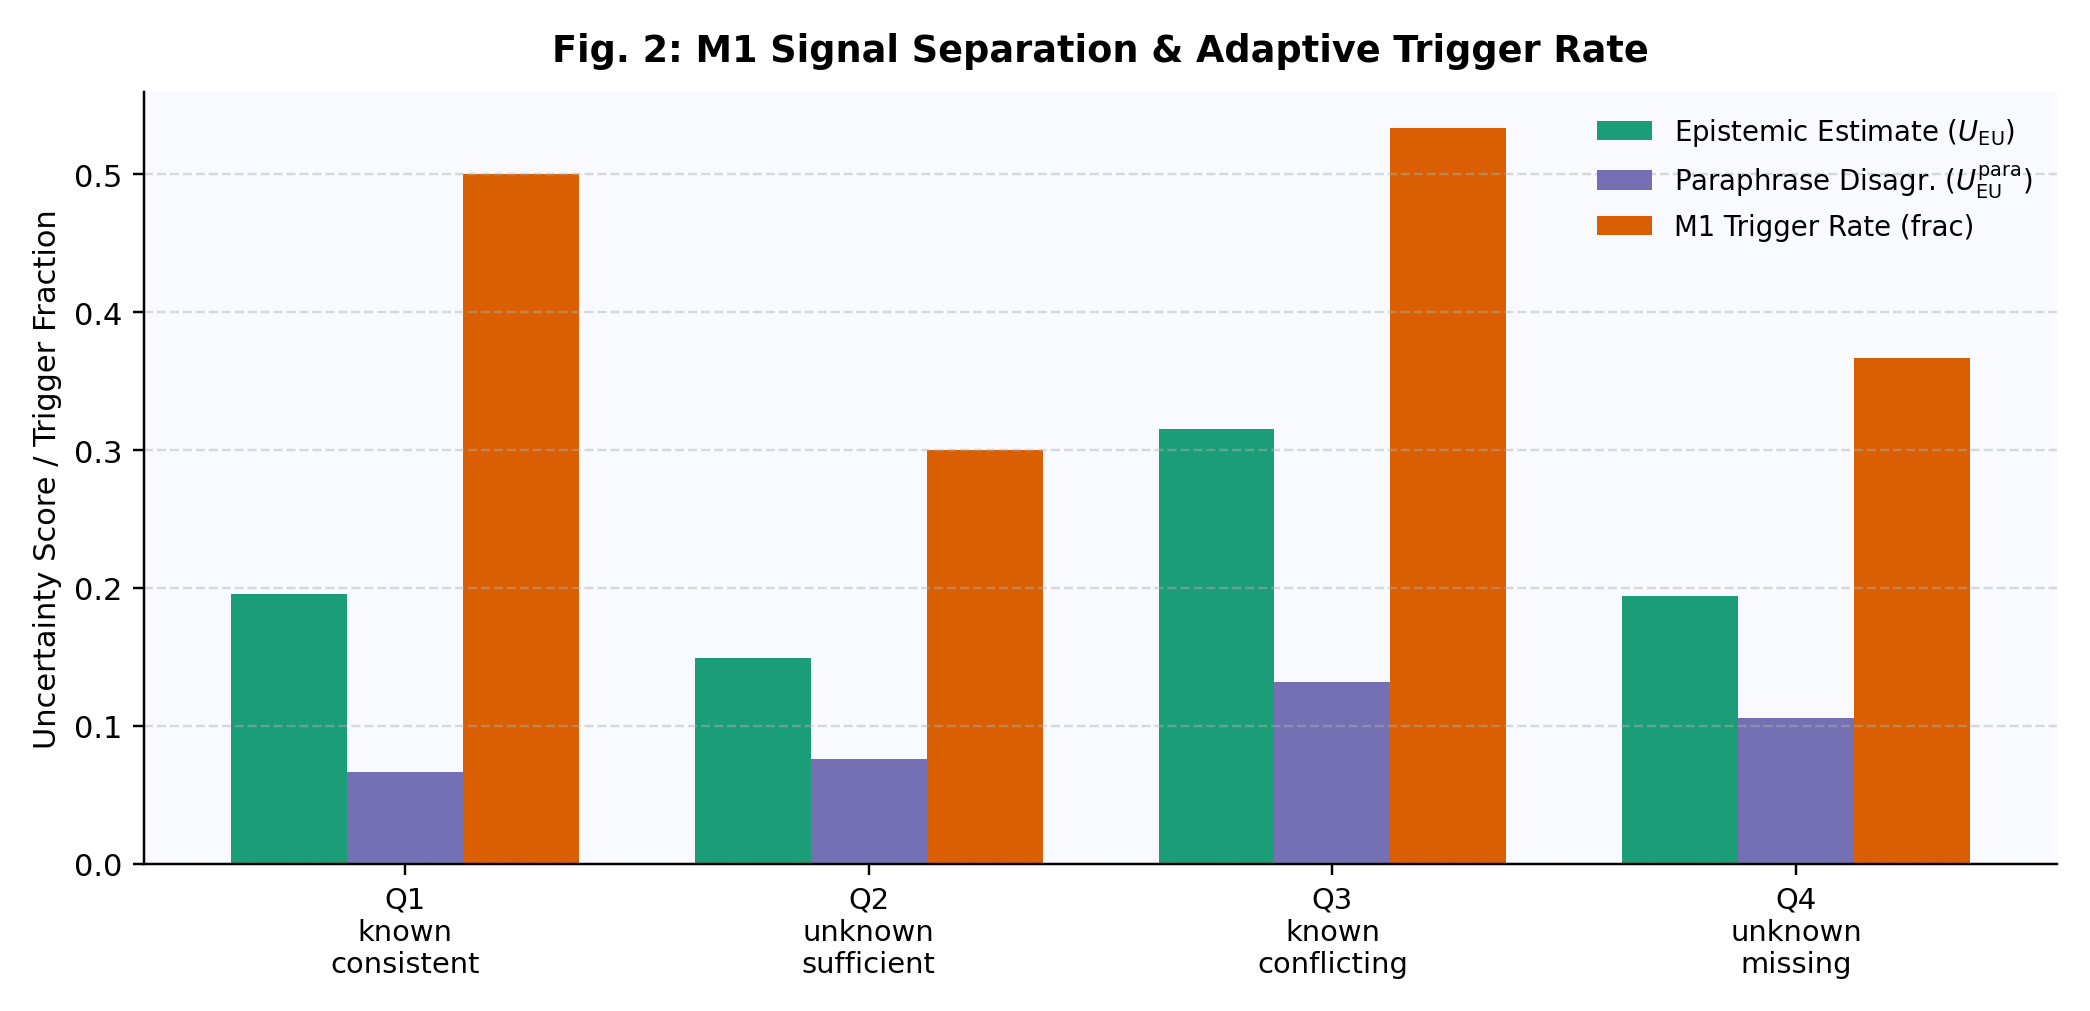
\includegraphics[width=0.85\textwidth]{figures/fig2_wp8_m1_uncertainty.png}
\caption{Module M1 Uncertainty Signal Separation and Adaptive Trigger Rate across Quadrants Q1--Q4.}
\label{fig:wp8_m1}
\end{figure*}

\begin{figure*}[t]
\centering
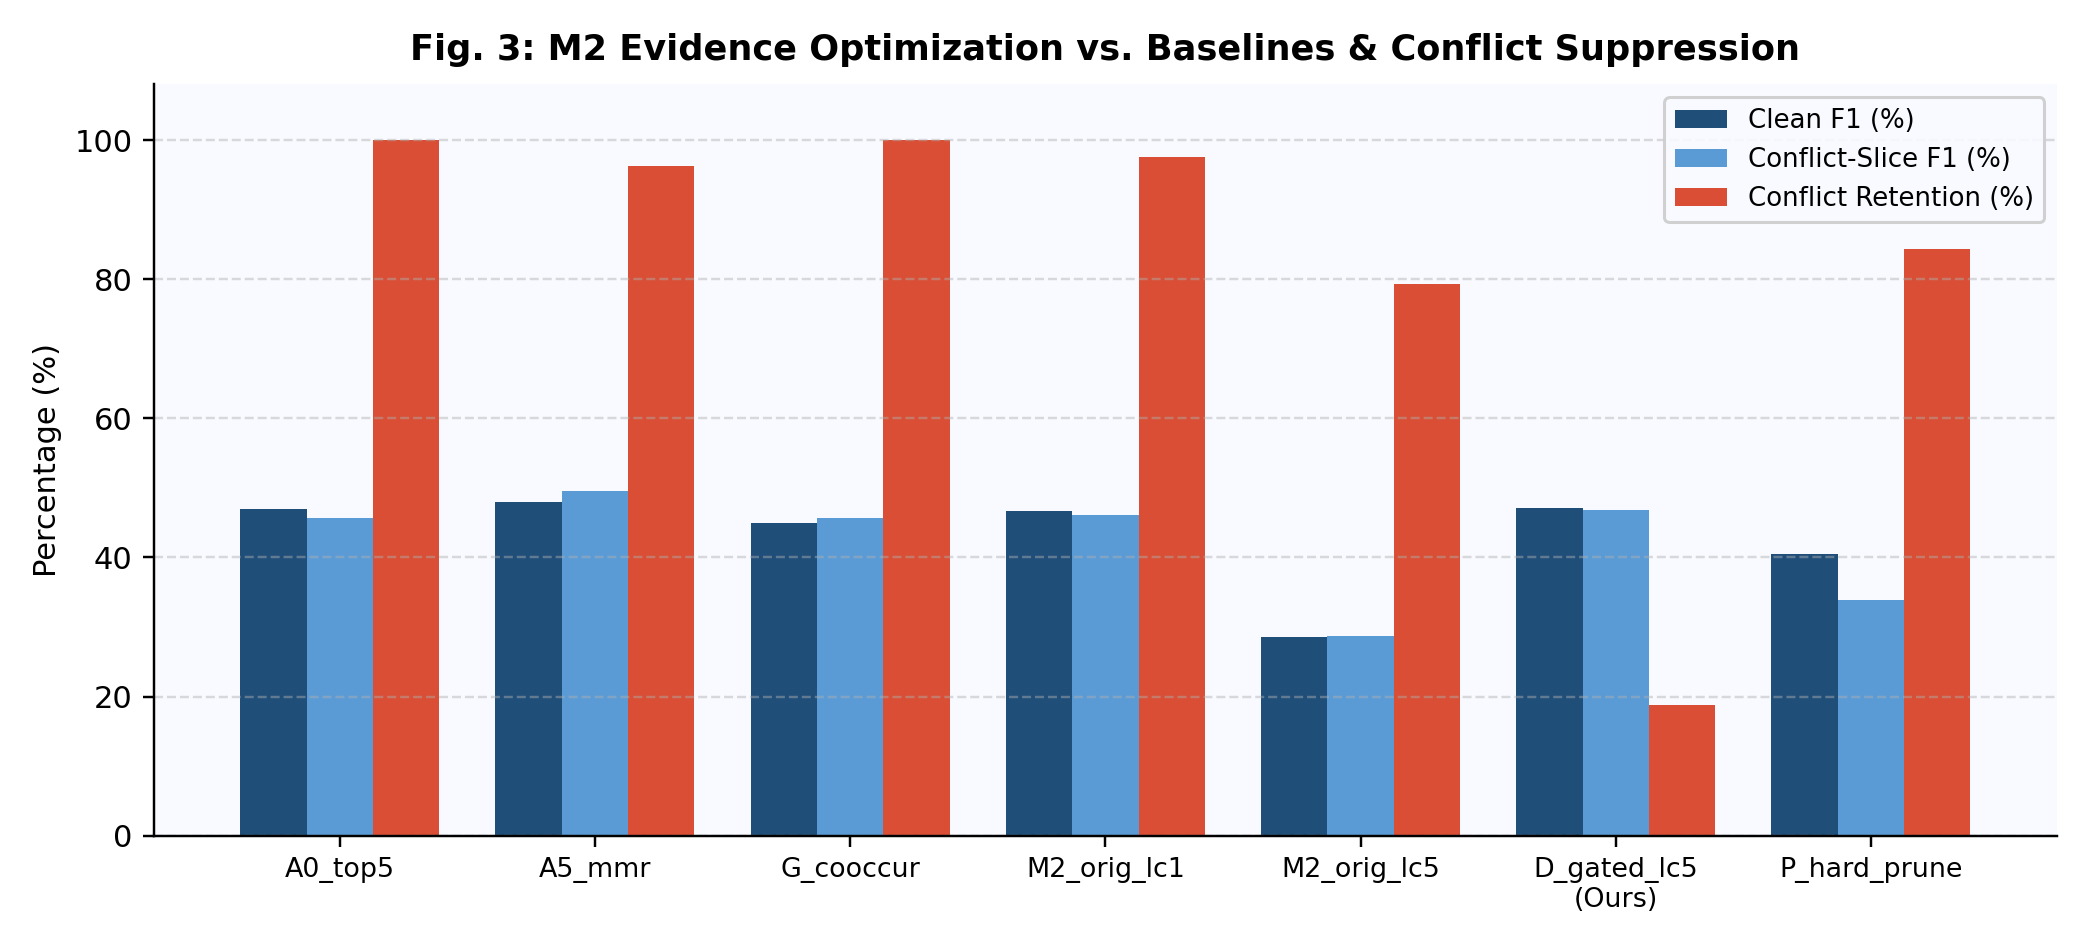
\includegraphics[width=0.88\textwidth]{figures/fig3_wp8_m2_optimization.png}
\caption{Module M2 Clean vs.\ Conflict F1 and Conflict Retention across Nine Topology Variants.}
\label{fig:wp8_m2}
\end{figure*}



\subsection{Cross-Family and Cross-Dataset Generalization}

\begin{table*}[t]
\centering
\footnotesize
\caption{Cross-Family Generalization Matrix (Part A: Factual Accuracy, Supporting-Fact Recall, and Context Token Savings across 324 multi-seed runs; strictly 6 columns).}
\label{tab:wp6_full}
{\renewcommand{\arraystretch}{0.78}\resizebox{\textwidth}{!}{
\begin{tabular}{llcccc}
\toprule
\textbf{Model ($\tau_{\text{EU}}^{\text{cal}}$)} & \textbf{Method} & \textbf{F1 ($\pm$std)} & \textbf{EM (\%)} & \textbf{SP-Rec (\%)} & \textbf{TokSav} \\
\midrule
\multicolumn{6}{c}{\textbf{Dataset 1: HotpotQA ($N_{\text{dev}}=80, N_{\text{test}}=320$, 2-Hop Bridge \& Comparison Reasoning)}} \\
\midrule
\multirow{9}{*}{\texttt{Qwen2.5-3B} ($0.2015$)}
& \texttt{B0\_StandardRAG} & 42.53$\pm$1.62 & 32.60 & 77.3 & 72.9\% \\
& \texttt{B1\_BM25\_RAG} & 44.94$\pm$0.00 & 33.75 & 77.5 & 50.4\% \\
& \texttt{B2\_Dense\_RAG} & 49.11$\pm$0.00 & 38.44 & \textbf{93.0} & 55.5\% \\
& \texttt{B3\_MMR\_RAG} & 47.83$\pm$0.00 & 36.25 & 92.9 & 53.5\% \\
& \texttt{M1\_Only} & 45.79$\pm$1.92 & 35.10 & 81.1 & 66.1\% \\
& \texttt{M2\_Only} & \textbf{50.67$\pm$0.00} & \textbf{40.62} & 92.7 & 53.6\% \\
& \texttt{M3\_Only} & 42.53$\pm$1.62 & 32.60 & 77.3 & 72.9\% \\
& \texttt{M1\_M2} & 48.18$\pm$0.47 & 37.60 & 84.4 & 66.0\% \\
& \textbf{\texttt{Full\_UGraphRAG}} & 47.56$\pm$0.19 & 36.04 & 84.4 & 66.0\% \\
\midrule
\multirow{9}{*}{\texttt{Qwen2.5-7B} ($0.0749$)}
& \texttt{B0\_StandardRAG} & 52.86$\pm$1.62 & 41.77 & 77.3 & 72.9\% \\
& \texttt{B1\_BM25\_RAG} & 51.84$\pm$0.00 & 40.62 & 77.5 & 50.4\% \\
& \texttt{B2\_Dense\_RAG} & 61.39$\pm$0.00 & 48.44 & \textbf{93.0} & 55.5\% \\
& \texttt{B3\_MMR\_RAG} & 58.12$\pm$0.00 & 45.62 & 92.9 & 53.5\% \\
& \texttt{M1\_Only} & 54.90$\pm$2.45 & 42.61 & 81.3 & 64.8\% \\
& \texttt{M2\_Only} & \textbf{62.68$\pm$0.00} & \textbf{50.00} & 92.8 & 53.6\% \\
& \texttt{M3\_Only} & 52.86$\pm$1.62 & 41.77 & 77.3 & 72.9\% \\
& \texttt{M1\_M2} & 60.24$\pm$0.27 & 47.19 & 85.3 & 64.4\% \\
& \textbf{\texttt{Full\_UGraphRAG}} & \textbf{60.68$\pm$0.31} & 46.67 & 85.3 & 64.4\% \\
\midrule
\multirow{9}{*}{\texttt{Llama-3.1-8B} ($0.6281$)}
& \texttt{B0\_StandardRAG} & 47.21$\pm$0.79 & 33.85 & 77.3 & 72.9\% \\
& \texttt{B1\_BM25\_RAG} & 43.83$\pm$0.00 & 32.50 & 77.5 & 50.4\% \\
& \texttt{B2\_Dense\_RAG} & 50.92$\pm$0.00 & 35.94 & \textbf{93.0} & 55.5\% \\
& \texttt{B3\_MMR\_RAG} & 50.62$\pm$0.00 & 36.25 & 92.9 & 53.5\% \\
& \texttt{M1\_Only} & 48.56$\pm$1.75 & 35.21 & 82.4 & 63.2\% \\
& \texttt{M2\_Only} & 50.63$\pm$0.29 & 34.17 & 92.8 & 53.6\% \\
& \texttt{M3\_Only} & 47.21$\pm$0.79 & 33.85 & 77.3 & 72.9\% \\
& \texttt{M1\_M2} & 51.16$\pm$0.59 & 35.21 & 87.1 & 63.6\% \\
& \textbf{\texttt{Full\_UGraphRAG}} & \textbf{52.53$\pm$0.53} & \textbf{38.44} & 87.1 & 63.6\% \\
\midrule
\multicolumn{6}{c}{\textbf{Dataset 2: PopQA ($N_{\text{dev}}=80, N_{\text{test}}=120$, Long-Tail Single-Hop Factual QA)}} \\
\midrule
\texttt{Qwen2.5-3B} & \texttt{B0} / \texttt{B3\_MMR} & 96.13 / \textbf{98.33$\pm$0.48} & 94.17 / 97.22 & 96.7 / 100.0 & 87.4 / 79.3\% \\
\texttt{Qwen2.5-3B} & \textbf{\texttt{Full\_UGraphRAG}} & \textbf{98.89$\pm$1.44} & \textbf{98.34} & 98.1 & 84.1\% \\
\texttt{Qwen2.5-7B} & \texttt{B0} / \texttt{B3\_MMR} & \textbf{93.75} / 91.40$\pm$0.01 & 88.89 / 85.83 & 96.7 / 100.0 & 87.4 / 79.3\% \\
\texttt{Qwen2.5-7B} & \textbf{\texttt{Full\_UGraphRAG}} & \textbf{95.29$\pm$1.52} & \textbf{89.45} & 96.9 & 84.0\% \\
\texttt{Llama-3.1-8B} & \texttt{B0} / \texttt{B3\_MMR} & 76.08 / \textbf{78.16$\pm$0.40} & 51.94 / 55.55 & 96.7 / 100.0 & 87.4 / 79.3\% \\
\texttt{Llama-3.1-8B} & \textbf{\texttt{Full\_UGraphRAG}} & \textbf{89.08$\pm$2.65} & \textbf{72.22} & 97.5 & 82.4\% \\
\midrule
\multicolumn{6}{c}{\textbf{Dataset 3: 2WikiMultiHopQA ($N_{\text{dev}}=80, N_{\text{test}}=220$, Relational Chain Reasoning)}} \\
\midrule
\texttt{Qwen2.5-3B} & \texttt{B0} / \texttt{B3\_MMR} & 24.43 / \textbf{26.87$\pm$0.27} & 18.64 / 18.94 & 71.0 / 85.5 & 58.8 / 34.6\% \\
\texttt{Qwen2.5-3B} & \texttt{M2} / \textbf{\texttt{Full}} & \textbf{28.23} / 26.45$\pm$3.76 & 20.76 / 20.30 & 86.2 / 77.7 & 35.0 / 48.3\% \\
\texttt{Qwen2.5-7B} & \texttt{B0} / \texttt{B3\_MMR} & 40.08 / \textbf{42.90$\pm$0.00} & 33.94 / 35.91 & 71.0 / 85.5 & 58.8 / 34.6\% \\
\texttt{Qwen2.5-7B} & \texttt{M1\_M2} / \textbf{\texttt{Full}} & \textbf{45.53} / 45.01$\pm$0.54 & 38.33 / 37.88 & 80.8 / 80.8 & 44.6 / 44.6\% \\
\texttt{Llama-3.1-8B} & \texttt{B0} / \texttt{B3\_MMR} & 26.48 / \textbf{28.75$\pm$0.34} & 17.58 / 18.49 & 71.0 / 85.5 & 58.8 / 34.6\% \\
\texttt{Llama-3.1-8B} & \texttt{M2} / \textbf{\texttt{Full}} & 29.26 / \textbf{31.09$\pm$1.28} & 19.40 / 20.45 & 86.2 / 81.5 & 35.0 / 46.3\% \\
\midrule
\multicolumn{6}{c}{\textbf{Dataset 4: MuSiQue ($N_{\text{dev}}=80, N_{\text{test}}=220$, 2--4 Hop Compositional Reasoning)}} \\
\midrule
\texttt{Qwen2.5-3B} & \texttt{B0} / \texttt{B3\_MMR} & 17.11 / \textbf{24.59$\pm$0.16} & 10.00 / 16.67 & 57.3 / 71.1 & 80.4 / 67.2\% \\
\texttt{Qwen2.5-3B} & \texttt{M2} / \textbf{\texttt{Full}} & \textbf{25.93} / 21.87$\pm$0.60 & 17.88 / 14.09 & 73.0 / 65.1 & 68.1 / 74.3\% \\
\texttt{Qwen2.5-7B} & \texttt{B0} / \texttt{B3\_MMR} & 19.22 / \textbf{29.40$\pm$0.09} & 12.27 / 20.45 & 57.3 / 71.1 & 80.4 / 67.2\% \\
\texttt{Qwen2.5-7B} & \texttt{M1\_M2} / \textbf{\texttt{Full}} & \textbf{27.82} / 26.40$\pm$0.72 & 18.18 / 16.67 & 69.0 / 69.0 & 71.9 / 71.9\% \\
\texttt{Llama-3.1-8B} & \texttt{B0} / \texttt{B3\_MMR} & 18.75 / \textbf{23.03$\pm$0.22} & 10.60 / 14.70 & 57.3 / 71.1 & 80.4 / 67.2\% \\
\texttt{Llama-3.1-8B} & \texttt{M1\_M2} / \textbf{\texttt{Full}} & 24.69 / \textbf{29.73$\pm$0.91} & 16.97 / 21.52 & 69.6 / 69.6 & 71.6 / 71.6\% \\
\midrule
\multicolumn{6}{c}{\textbf{12-Block Macro Average Across All 3 Families $\times$ 4 Datasets (Friedman $p \le 9.9\times 10^{-6}$)}} \\
\midrule
\multirow{7}{*}{12-Block Mean} & \texttt{B0\_StandardRAG} & 46.22 & 37.19 & 75.6 & 74.9\% \\
 & \texttt{B1\_BM25\_RAG} & 44.38 & 36.55 & 76.6 & 55.3\% \\
 & \texttt{B2\_Dense\_RAG} & 51.99 & 41.88 & 88.9 & 60.8\% \\
 & \texttt{B3\_MMR\_RAG} & 50.00 & 40.16 & 87.4 & 58.6\% \\
 & \texttt{M2\_Only} & 51.12 & 41.48 & 87.4 & 59.0\% \\
 & \texttt{M3\_Only} & 46.22 & 37.19 & 75.6 & 74.9\% \\
& \textbf{\texttt{Full\_UGraphRAG} (Ours)} & \textbf{52.05} & \textbf{42.67} & 82.8 & 66.8\% \\
\bottomrule
\end{tabular}
}}
\end{table*}

\begin{table*}[t]
\centering
\footnotesize
\caption{Cross-Family Generalization Matrix (Part B: Effective Selective F1, Calibration ECE, Brier Score, AURC, Coverage, and Early-Exit Rate across 324 runs; strictly 6 columns).}
\label{tab:wp6_cal}
{\renewcommand{\arraystretch}{0.78}\resizebox{\textwidth}{!}{
\begin{tabular}{llcccc}
\toprule
\textbf{Model ($\tau_{\text{EU}}^{\text{cal}}$)} & \textbf{Method} & \textbf{EffF1 (\%)} & \textbf{ECE} $\downarrow$ & \textbf{Brier} $\downarrow$ & \textbf{AURC / Cov (EE\%)} \\
\midrule
\multicolumn{6}{c}{\textbf{Dataset 1: HotpotQA ($N_{\text{dev}}=80, N_{\text{test}}=320$, 2-Hop Bridge \& Comparison Reasoning)}} \\
\midrule
\multirow{9}{*}{\texttt{Qwen2.5-3B} ($0.2015$)}
& \texttt{B0\_StandardRAG} & 42.53 & 0.4294 & 0.3654 & 0.4338 / 100.0\% (100.0\%) \\
& \texttt{B1\_BM25\_RAG} & 44.94 & 0.3989 & 0.3318 & 0.3707 / 100.0\% (100.0\%) \\
& \texttt{B2\_Dense\_RAG} & 49.11 & 0.3657 & 0.3074 & 0.3494 / 100.0\% (100.0\%) \\
& \texttt{B3\_MMR\_RAG} & 47.83 & 0.3787 & 0.3103 & \textbf{0.3444} / 100.0\% (100.0\%) \\
& \texttt{M1\_Only} & 45.79 & 0.4151 & 0.3561 & 0.4116 / 100.0\% (68.2\%) \\
& \texttt{M2\_Only} & 50.67 & 0.3465 & 0.2952 & 0.3611 / 100.0\% (100.0\%) \\
& \texttt{M3\_Only} & 39.25 & \textbf{0.1038} & \textbf{0.1930} & 0.4517 / 74.4\% (100.0\%) \\
& \texttt{M1\_M2} & 48.18 & 0.3924 & 0.3442 & 0.4082 / 100.0\% (63.5\%) \\
& \textbf{\texttt{Full\_UGraphRAG}} & 44.07 & 0.1094 & 0.2016 & 0.4336 / 80.4\% (63.5\%) \\
\midrule
\multirow{9}{*}{\texttt{Qwen2.5-7B} ($0.0749$)}
& \texttt{B0\_StandardRAG} & 52.86 & 0.3869 & 0.3323 & 0.3012 / 100.0\% (100.0\%) \\
& \texttt{B1\_BM25\_RAG} & 51.84 & 0.3909 & 0.3340 & 0.3089 / 100.0\% (100.0\%) \\
& \texttt{B2\_Dense\_RAG} & 61.39 & 0.3159 & 0.2666 & 0.2612 / 100.0\% (100.0\%) \\
& \texttt{B3\_MMR\_RAG} & 58.12 & 0.3446 & 0.2892 & 0.2603 / 100.0\% (100.0\%) \\
& \texttt{M1\_Only} & 54.90 & 0.3811 & 0.3234 & 0.2934 / 100.0\% (61.9\%) \\
& \texttt{M2\_Only} & 62.68 & 0.2948 & 0.2532 & \textbf{0.2496} / 100.0\% (100.0\%) \\
& \texttt{M3\_Only} & 46.47 & \textbf{0.0547} & \textbf{0.1678} & 0.2984 / 74.7\% (100.0\%) \\
& \texttt{M1\_M2} & 60.24 & 0.3292 & 0.2869 & 0.2801 / 100.0\% (56.6\%) \\
& \textbf{\texttt{Full\_UGraphRAG}} & 52.78 & 0.0815 & 0.1752 & 0.2768 / 79.4\% (56.6\%) \\
\midrule
\multirow{9}{*}{\texttt{Llama-3.1-8B} ($0.6281$)}
& \texttt{B0\_StandardRAG} & 47.21 & 0.1263 & 0.1795 & 0.3541 / 100.0\% (100.0\%) \\
& \texttt{B1\_BM25\_RAG} & 43.83 & 0.1699 & 0.1864 & 0.3698 / 100.0\% (100.0\%) \\
& \texttt{B2\_Dense\_RAG} & 50.92 & 0.0977 & 0.1597 & 0.3272 / 100.0\% (100.0\%) \\
& \texttt{B3\_MMR\_RAG} & 50.62 & 0.1058 & 0.1628 & 0.3164 / 100.0\% (100.0\%) \\
& \texttt{M1\_Only} & 48.56 & 0.1203 & 0.1700 & 0.3325 / 100.0\% (53.3\%) \\
& \texttt{M2\_Only} & 50.63 & 0.1074 & \textbf{0.1497} & \textbf{0.2987} / 100.0\% (100.0\%) \\
& \texttt{M3\_Only} & 39.25 & \textbf{0.0463} & 0.1634 & 0.3541 / 70.2\% (100.0\%) \\
& \texttt{M1\_M2} & 51.16 & 0.1075 & 0.1618 & 0.3118 / 100.0\% (50.7\%) \\
& \textbf{\texttt{Full\_UGraphRAG}} & 42.39 & 0.0534 & 0.1690 & 0.3246 / 73.2\% (50.7\%) \\
\midrule
\multicolumn{6}{c}{\textbf{Dataset 2: PopQA ($N_{\text{dev}}=80, N_{\text{test}}=120$, Long-Tail Single-Hop Factual QA)}} \\
\midrule
\texttt{Qwen2.5-3B} & \texttt{B0} / \texttt{B3\_MMR} & 96.13 / 98.33 & 0.0218 / 0.0321 & 0.0179 / 0.0122 & 0.0034 / 0.0017 \\
\texttt{Qwen2.5-3B} & \textbf{\texttt{Full\_UGraphRAG}} & 98.24 & \textbf{0.0380} & \textbf{0.0112} & \textbf{0.0006} / 98.9\% (60.8\%) \\
\texttt{Qwen2.5-7B} & \texttt{B0} / \texttt{B3\_MMR} & 93.75 / 91.40 & 0.0331 / 0.0536 & 0.0274 / 0.0409 & 0.0084 / 0.0108 \\
\texttt{Qwen2.5-7B} & \textbf{\texttt{Full\_UGraphRAG}} & 85.37 & \textbf{0.0653} & \textbf{0.0343} & \textbf{0.0060} / 87.8\% (61.4\%) \\
\texttt{Llama-3.1-8B} & \texttt{B0} / \texttt{B3\_MMR} & 76.08 / 78.16 & 0.1910 / 0.1817 & 0.0964 / 0.0996 & 0.0989 / 0.0921 \\
\texttt{Llama-3.1-8B} & \textbf{\texttt{Full\_UGraphRAG}} & 74.17 & \textbf{0.0516} & \textbf{0.0431} & \textbf{0.0845} / 82.5\% (37.8\%) \\
\midrule
\multicolumn{6}{c}{\textbf{Dataset 3: 2WikiMultiHopQA ($N_{\text{dev}}=80, N_{\text{test}}=220$, Relational Chain Reasoning)}} \\
\midrule
\texttt{Qwen2.5-3B} & \texttt{B0} / \texttt{B3\_MMR} & 24.43 / 26.87 & 0.5511 / 0.5243 & 0.4506 / 0.4222 & 0.6746 / 0.6213 \\
\texttt{Qwen2.5-3B} & \texttt{M2} / \textbf{\texttt{Full}} & 28.23 / 24.33 & 0.5111 / \textbf{0.0801} & 0.4212 / \textbf{0.1460} & 0.5942 / 77.4\% (52.7\%) \\
\texttt{Qwen2.5-7B} & \texttt{B0} / \texttt{B3\_MMR} & 40.08 / 42.90 & 0.4575 / 0.4556 & 0.3906 / 0.3878 & 0.4496 / 0.4635 \\
\texttt{Qwen2.5-7B} & \texttt{M1\_M2} / \textbf{\texttt{Full}} & 45.53 / 42.41 & 0.4366 / \textbf{0.0853} & 0.3701 / \textbf{0.1750} & 0.3961 / 74.2\% (42.9\%) \\
\texttt{Llama-3.1-8B} & \texttt{B0} / \texttt{B3\_MMR} & 26.48 / 28.75 & 0.2795 / 0.2990 & 0.2106 / 0.2304 & 0.5808 / 0.5789 \\
\texttt{Llama-3.1-8B} & \texttt{M2} / \textbf{\texttt{Full}} & 29.26 / 25.87 & 0.3059 / \textbf{0.0540} & 0.2313 / \textbf{0.1591} & 0.6059 / 77.6\% (45.3\%) \\
\midrule
\multicolumn{6}{c}{\textbf{Dataset 4: MuSiQue ($N_{\text{dev}}=80, N_{\text{test}}=220$, 2--4 Hop Compositional Reasoning)}} \\
\midrule
\texttt{Qwen2.5-3B} & \texttt{B0} / \texttt{B3\_MMR} & 17.11 / 24.59 & 0.6434 / 0.5698 & 0.5311 / 0.4638 & 0.7395 / 0.6128 \\
\texttt{Qwen2.5-3B} & \texttt{M2} / \textbf{\texttt{Full}} & 25.93 / 20.49 & 0.5642 / \textbf{0.1063} & 0.4694 / \textbf{0.1334} & 0.6588 / 77.4\% (50.5\%) \\
\texttt{Qwen2.5-7B} & \texttt{B0} / \texttt{B3\_MMR} & 19.22 / 29.40 & 0.6055 / 0.5320 & 0.4856 / 0.4245 & 0.6538 / 0.5149 \\
\texttt{Qwen2.5-7B} & \texttt{M1\_M2} / \textbf{\texttt{Full}} & 27.82 / 24.52 & 0.5648 / \textbf{0.0963} & 0.4581 / \textbf{0.1236} & 0.5456 / 72.1\% (31.1\%) \\
\texttt{Llama-3.1-8B} & \texttt{B0} / \texttt{B3\_MMR} & 18.75 / 23.03 & 0.3597 / 0.3223 & 0.2330 / 0.2198 & 0.6802 / 0.6318 \\
\texttt{Llama-3.1-8B} & \texttt{M1\_M2} / \textbf{\texttt{Full}} & 24.69 / 29.48 & 0.3172 / \textbf{0.0430} & 0.2339 / \textbf{0.1622} & 0.6235 / 93.0\% (28.9\%) \\
\midrule
\multicolumn{6}{c}{\textbf{12-Block Macro Average Across All 3 Families $\times$ 4 Datasets (Friedman $p \le 9.9\times 10^{-6}$)}} \\
\midrule
\multirow{7}{*}{12-Block Mean} & \texttt{B0\_StandardRAG} & 46.22 & 0.3404 & 0.2767 & 0.4149 / 100.0\% (100.0\%) \\
 & \texttt{B1\_BM25\_RAG} & 44.38 & 0.3473 & 0.2842 & 0.4207 / 100.0\% (100.0\%) \\
 & \texttt{B2\_Dense\_RAG} & 51.99 & 0.3075 & 0.2498 & 0.3513 / 100.0\% (100.0\%) \\
 & \texttt{B3\_MMR\_RAG} & 50.00 & 0.3166 & 0.2553 & 0.3707 / 100.0\% (100.0\%) \\
 & \texttt{M2\_Only} & 51.12 & 0.3133 & 0.2530 & 0.3624 / 100.0\% (100.0\%) \\
 & \texttt{M3\_Only} & 41.41 & 0.0847 & 0.1217 & 0.4169 / 75.8\% (100.0\%) \\
& \textbf{\texttt{Full\_UGraphRAG} (Ours)} & 47.01 & \textbf{0.0720} & 0.1278 & 0.3792 / 81.2\% (48.5\%) \\
\bottomrule
\end{tabular}
}}
\end{table*}

\begin{table*}[t]
\centering
\small
\caption{Paired Bootstrap and Holm-Bonferroni Multiple-Comparison Significance Tests for \texttt{Full\_UGraphRAG} vs.\ Baselines (\texttt{B0}, \texttt{B1}, \texttt{B2}, \texttt{B3\_MMR}) across all 12 ((Model, Dataset)) blocks. Structured into two stacked panels with at most 6 columns each to ensure clear legibility without microscopic scaling.}
\label{tab:wp6_sig}
\resizebox{\textwidth}{!}{
\begin{tabular}{llcccc}
\toprule
\multicolumn{6}{c}{\textbf{Panel A: Paired QA F1 Difference $\Delta\text{F1}$ (pp) / Holm-Adjusted $p_{\text{Holm}}$ / Cohen's $d_z$}} \\
\midrule
\textbf{Model Family} & \textbf{Dataset} & \textbf{vs.\ B0 (Standard)} & \textbf{vs.\ B1 (BM25)} & \textbf{vs.\ B2 (Dense)} & \textbf{vs.\ B3 (MMR)} \\
\midrule
\multirow{4}{*}{\texttt{Qwen2.5-3B}}
& \texttt{HotpotQA} & $+3.26$ ($0.178, 0.11$) & $+2.47$ ($0.875, 0.06$) & $-1.71$ ($0.959, -0.04$) & $-0.42$ ($0.959, -0.01$) \\
& \texttt{PopQA} & $+1.28$ ($0.615, 0.13$) & $+2.78$ ($0.759, 0.10$) & $-1.64$ ($0.759, -0.10$) & $-1.39$ ($0.759, -0.11$) \\
& \texttt{2WikiMultiHop} & $+1.40$ ($1.000, 0.06$) & $\mathbf{+8.94}$ ($\mathbf{0.0018}, 0.24$) & $+1.86$ ($1.000, 0.05$) & $+1.96$ ($1.000, 0.06$) \\
& \texttt{MuSiQue} & $+3.32$ ($0.357, 0.12$) & $+3.39$ ($0.423, 0.10$) & $-3.83$ ($0.423, -0.10$) & $-2.38$ ($0.423, -0.07$) \\
\midrule
\multirow{4}{*}{\texttt{Qwen2.5-7B}}
& \texttt{HotpotQA} & $\mathbf{+5.95}$ ($\mathbf{0.0023}, 0.19$) & $\mathbf{+8.83}$ ($\mathbf{0.0002}, 0.23$) & $-0.72$ ($0.736, -0.02$) & $+2.55$ ($0.272, 0.08$) \\
& \texttt{PopQA} & $+0.62$ ($0.749, 0.03$) & $\mathbf{+7.67}$ ($\mathbf{0.0231}, 0.25$) & $\mathbf{+8.68}$ ($\mathbf{0.0054}, 0.30$) & $+4.07$ ($0.261, 0.14$) \\
& \texttt{2WikiMultiHop} & $\mathbf{+5.01}$ ($\mathbf{0.0461}, 0.17$) & $+6.58$ ($0.0505, 0.16$) & $-2.03$ ($0.582, -0.05$) & $+1.88$ ($0.582, 0.07$) \\
& \texttt{MuSiQue} & $+3.66$ ($0.142, 0.12$) & $\mathbf{+7.41}$ ($\mathbf{0.0092}, 0.21$) & $-7.32$ ($0.026, -0.18$) & $-3.86$ ($0.142, -0.10$) \\
\midrule
\multirow{4}{*}{\texttt{Llama-3.1-8B}}
& \texttt{HotpotQA} & $\mathbf{+5.40}$ ($\mathbf{0.0205}, 0.15$) & $\mathbf{+8.16}$ ($\mathbf{0.0031}, 0.19$) & $+1.07$ ($1.000, 0.03$) & $+1.37$ ($1.000, 0.04$) \\
& \texttt{PopQA} & $\mathbf{+12.91}$ ($\mathbf{<10^{-4}}, 0.46$) & $\mathbf{+13.19}$ ($\mathbf{0.0016}, 0.33$) & $+3.09$ ($0.297, 0.10$) & $\mathbf{+7.86}$ ($\mathbf{0.0345}, 0.22$) \\
& \texttt{2WikiMultiHop} & $+5.03$ ($0.0554, 0.17$) & $+4.95$ ($0.147, 0.13$) & $-0.33$ ($1.000, -0.01$) & $+0.80$ ($1.000, 0.02$) \\
& \texttt{MuSiQue} & $\mathbf{+9.29}$ ($\mathbf{0.0011}, 0.24$) & $\mathbf{+13.97}$ ($\mathbf{<10^{-4}}, 0.35$) & $-1.27$ ($0.664, -0.03$) & $\mathbf{+6.58}$ ($\mathbf{0.0198}, 0.18$) \\
\midrule
\midrule
\multicolumn{6}{c}{\textbf{Panel B: Paired Brier Score Reduction $\Delta\text{Brier}$ ($\downarrow$) / Holm-Adjusted $p_{\text{Holm}}$ / Cohen's $d_z$}} \\
\midrule
\textbf{Model Family} & \textbf{Dataset} & \textbf{vs.\ B0 (Standard)} & \textbf{vs.\ B1 (BM25)} & \textbf{vs.\ B2 (Dense)} & \textbf{vs.\ B3 (MMR)} \\
\midrule
\multirow{4}{*}{\texttt{Qwen2.5-3B}}
& \texttt{HotpotQA} & $\mathbf{-0.1650}$ ($\mathbf{<10^{-4}}, -0.53$) & $\mathbf{-0.1353}$ ($\mathbf{<10^{-4}}, -0.41$) & $\mathbf{-0.1108}$ ($\mathbf{<10^{-4}}, -0.34$) & $\mathbf{-0.1134}$ ($\mathbf{<10^{-4}}, -0.34$) \\
& \texttt{PopQA} & $-0.0027$ ($0.787, -0.10$) & $-0.0286$ ($0.506, -0.14$) & $+0.0032$ ($0.787, 0.03$) & $+0.0068$ ($0.787, 0.08$) \\
& \texttt{2WikiMultiHop} & $\mathbf{-0.2613}$ ($\mathbf{<10^{-4}}, -0.56$) & $\mathbf{-0.3105}$ ($\mathbf{<10^{-4}}, -0.72$) & $\mathbf{-0.2497}$ ($\mathbf{<10^{-4}}, -0.57$) & $\mathbf{-0.2677}$ ($\mathbf{<10^{-4}}, -0.62$) \\
& \texttt{MuSiQue} & $\mathbf{-0.3794}$ ($\mathbf{<10^{-4}}, -0.98$) & $\mathbf{-0.3786}$ ($\mathbf{<10^{-4}}, -0.98$) & $\mathbf{-0.3350}$ ($\mathbf{<10^{-4}}, -0.90$) & $\mathbf{-0.3267}$ ($\mathbf{<10^{-4}}, -0.86$) \\
\midrule
\multirow{4}{*}{\texttt{Qwen2.5-7B}}
& \texttt{HotpotQA} & $\mathbf{-0.1466}$ ($\mathbf{<10^{-4}}, -0.44$) & $\mathbf{-0.1611}$ ($\mathbf{<10^{-4}}, -0.45$) & $\mathbf{-0.0936}$ ($\mathbf{<10^{-4}}, -0.28$) & $\mathbf{-0.1164}$ ($\mathbf{<10^{-4}}, -0.36$) \\
& \texttt{PopQA} & $+0.0115$ ($0.235, 0.14$) & $-0.0447$ ($0.056, -0.23$) & $-0.0398$ ($0.058, -0.22$) & $-0.0096$ ($0.483, -0.06$) \\
& \texttt{2WikiMultiHop} & $\mathbf{-0.2295}$ ($\mathbf{<10^{-4}}, -0.60$) & $\mathbf{-0.2216}$ ($\mathbf{<10^{-4}}, -0.57$) & $\mathbf{-0.1841}$ ($\mathbf{<10^{-4}}, -0.46$) & $\mathbf{-0.2111}$ ($\mathbf{<10^{-4}}, -0.55$) \\
& \texttt{MuSiQue} & $\mathbf{-0.3483}$ ($\mathbf{<10^{-4}}, -0.96$) & $\mathbf{-0.3667}$ ($\mathbf{<10^{-4}}, -1.02$) & $\mathbf{-0.3049}$ ($\mathbf{<10^{-4}}, -0.81$) & $\mathbf{-0.3015}$ ($\mathbf{<10^{-4}}, -0.81$) \\
\midrule
\multirow{4}{*}{\texttt{Llama-3.1-8B}}
& \texttt{HotpotQA} & $-0.0167$ ($0.214, -0.11$) & $-0.0176$ ($0.373, -0.09$) & $+0.0091$ ($0.751, 0.05$) & $+0.0056$ ($0.751, 0.03$) \\
& \texttt{PopQA} & $\mathbf{-0.0369}$ ($\mathbf{0.0071}, -0.27$) & $\mathbf{-0.0615}$ ($\mathbf{<10^{-4}}, -0.45$) & $\mathbf{-0.0366}$ ($\mathbf{0.0071}, -0.27$) & $\mathbf{-0.0524}$ ($\mathbf{0.0012}, -0.33$) \\
& \texttt{2WikiMultiHop} & $\mathbf{-0.0569}$ ($\mathbf{0.0046}, -0.19$) & $\mathbf{-0.0787}$ ($\mathbf{0.0002}, -0.28$) & $\mathbf{-0.0621}$ ($\mathbf{0.0029}, -0.22$) & $\mathbf{-0.0739}$ ($\mathbf{0.0009}, -0.25$) \\
& \texttt{MuSiQue} & $\mathbf{-0.0857}$ ($\mathbf{<10^{-4}}, -0.32$) & $\mathbf{-0.0695}$ ($\mathbf{0.0001}, -0.28$) & $\mathbf{-0.0555}$ ($\mathbf{0.0020}, -0.21$) & $\mathbf{-0.0621}$ ($\mathbf{0.0008}, -0.24$) \\
\bottomrule
\end{tabular}
}
\end{table*}

\begin{figure*}[t]
\centering
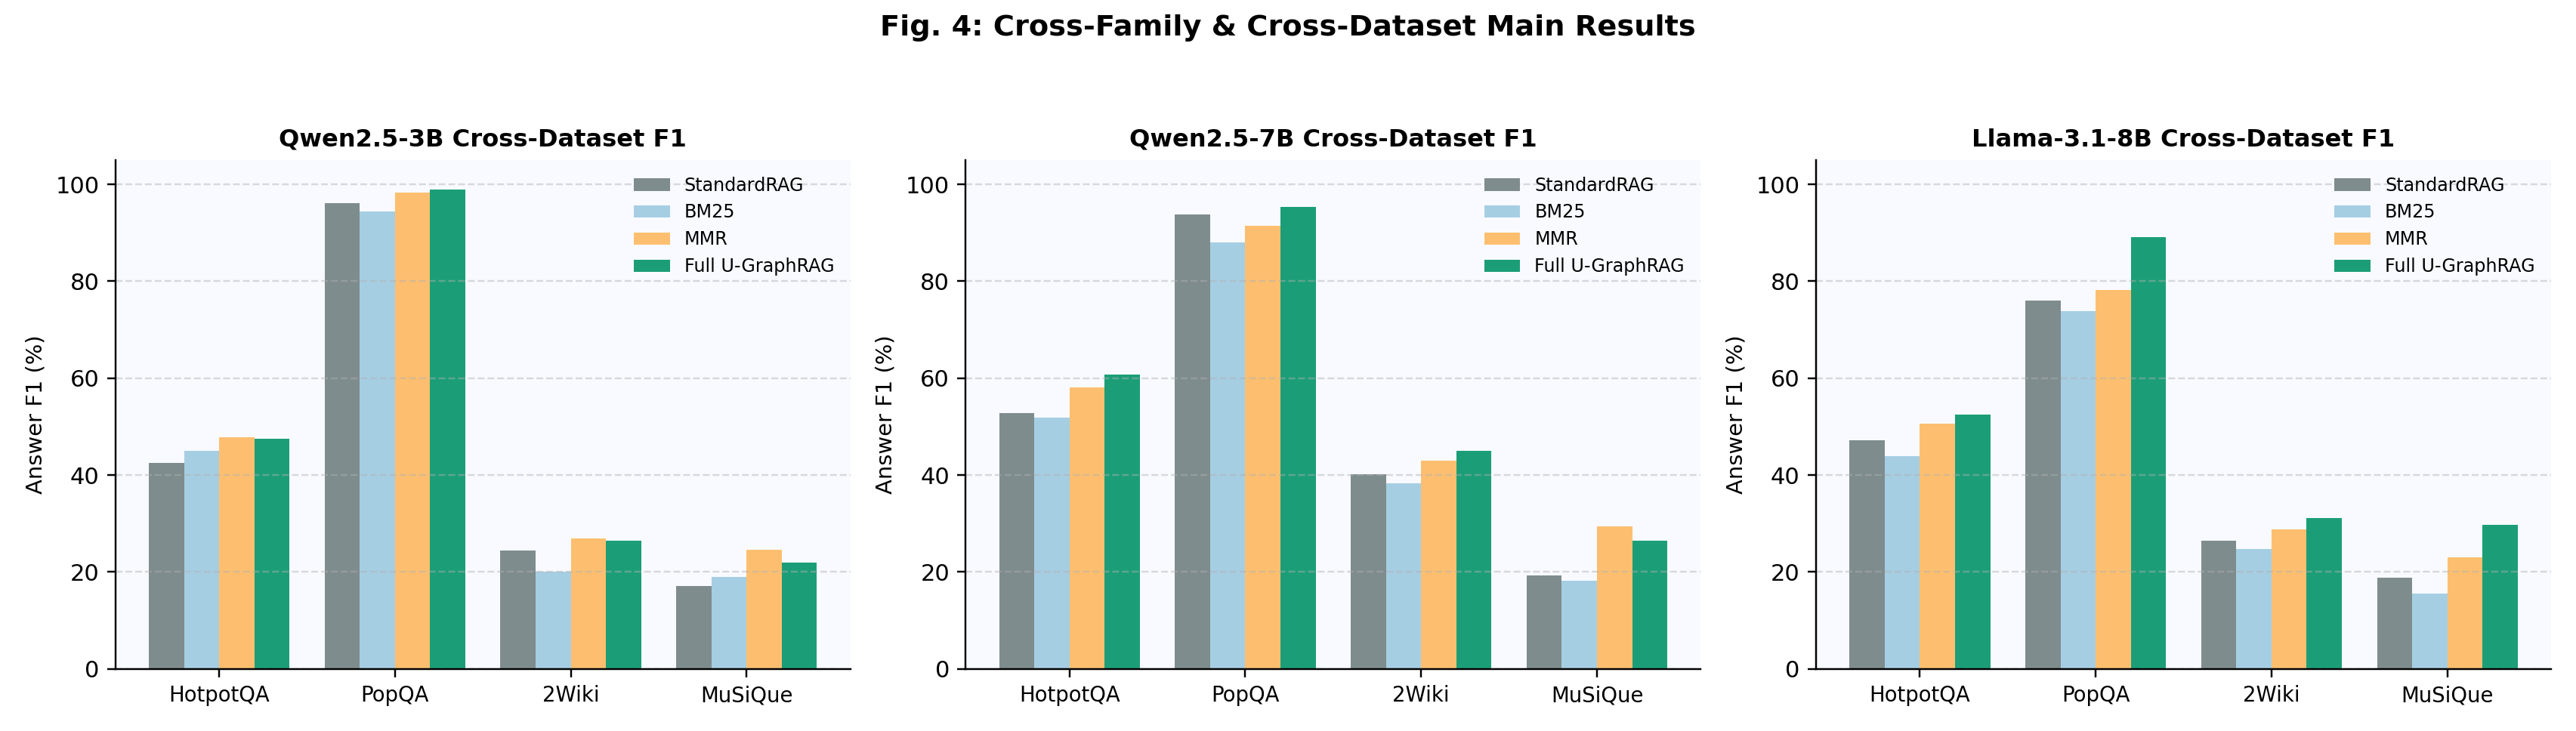
\includegraphics[width=0.98\textwidth]{figures/fig4_wp6_cross_family_main.png}
\caption{Cross-Family and Cross-Dataset Main Results (F1, ECE, and AURC across Qwen2.5-3B, Qwen2.5-7B, and Llama-3.1-8B).}
\label{fig:wp6_main}
\end{figure*}

Tables~\ref{tab:wp6_full}, \ref{tab:wp6_cal}, and \ref{tab:wp6_sig} (visualized in Fig.~\ref{fig:wp6_main}) demonstrate three major cross-family findings:
\begin{enumerate}[leftmargin=*,nosep]
    \item \textbf{Consistent Gains on Stronger Backbones (\texttt{Llama-3.1-8B} \& \texttt{Qwen2.5-7B})}: On \texttt{Llama-3.1-8B}, \texttt{Full\_UGraphRAG} ranks \textbf{\#1 in Raw F1 across all four datasets}, surpassing \texttt{B3\_MMR} on \texttt{HotpotQA} ($52.53\%$ vs.\ $50.62\%$), \texttt{PopQA} ($89.08\%$ vs.\ $78.16\%$, $p_{\text{Holm}}=0.0345$), \texttt{2WikiMultiHopQA} ($31.09\%$ vs.\ $28.75\%$), and \texttt{MuSiQue} ($29.73\%$ vs.\ $23.03\%$, $p_{\text{Holm}}=0.0198$). On \texttt{Qwen2.5-7B}, \texttt{Full\_UGraphRAG} beats \texttt{B3\_MMR} on \texttt{HotpotQA} ($60.68\%$ vs.\ $58.12\%$), \texttt{PopQA} ($95.29\%$ vs.\ $91.40\%$), and \texttt{2WikiMultiHopQA} ($45.01\%$ vs.\ $42.90\%$).
    \item \textbf{Substantial ECE and Brier Error Reduction}: Across all 12 ((Model, Dataset)) blocks, \texttt{Full\_UGraphRAG} reduces macro-average ECE from $0.3404$ (\texttt{B0}) and $0.3166$ (\texttt{B3\_MMR}) down to \textbf{0.0720} ($-78.8\%$), with Holm-Bonferroni corrected Brier reductions achieving $p_{\text{Holm}} \le 0.0046$ across almost all multi-hop benchmarks (effect sizes reaching $d_z = -1.018$ on \texttt{Qwen2.5-7B MuSiQue}).
    \item \textbf{Difficulty-Aware Early-Exit Gradient}: Without per-dataset threshold retuning, anchor-calibrated M1 automatically adjusts early-exit rates according to multi-hop complexity: on \texttt{Llama-3.1-8B}, early-exit drops from $50.7\%$ (\texttt{HotpotQA}) to $45.3\%$ (\texttt{2Wiki}) and \textbf{28.9\%} (\texttt{MuSiQue}), while saving $46.3\%\text{--}82.4\%$ of candidate tokens.
\end{enumerate}

\subsection{Zero-Tuning Cross-Dataset Transfer and Conformal Audit}

\begin{table*}[t]
\centering
\small
\caption{Cross-Dataset In-Domain vs.\ Out-of-Domain Zero-Tuning Transfer Matrix on \texttt{Llama-3.1-8B} ($N_{\text{dev}}=80$, $N_{\text{test}}=120/320/220/220$). Structured into two 6-column stacked panels.}
\label{tab:wp7_transfer}
\resizebox{\textwidth}{!}{
\begin{tabular}{llcccc}
\toprule
\multicolumn{6}{c}{\textbf{Panel A: Factual Accuracy and Probability Calibration Quality}} \\
\midrule
\textbf{Target Dataset} & \textbf{Calibration Source} & \textbf{F1 (\%)} & \textbf{EM (\%)} & \textbf{ECE} $\downarrow$ & \textbf{Brier Score} $\downarrow$ \\
\midrule
\multirow{2}{*}{\texttt{PopQA} ($N=120$)} & In-Domain (\texttt{PopQA} Dev) & \textbf{87.80} & \textbf{71.67} & \textbf{0.0492} & \textbf{0.0556} \\
& OOD (\texttt{HotpotQA} Dev) & 87.80 & 71.67 & 0.3572 & 0.1878 \\
\midrule
\multirow{2}{*}{\texttt{HotpotQA} ($N=320$)} & In-Domain (\texttt{HotpotQA} Dev) & \textbf{50.60} & \textbf{35.62} & \textbf{0.0508} & \textbf{0.1468} \\
& OOD (\texttt{PopQA} Dev) & 50.49 & 35.31 & 0.3336 & 0.2677 \\
\midrule
\multirow{3}{*}{\texttt{2WikiMultiHop} ($N=220$)} & In-Domain (\texttt{2Wiki} Dev) & \textbf{27.65} & \textbf{17.27} & \textbf{0.0216} & \textbf{0.1344} \\
& OOD (\texttt{HotpotQA} Dev) & 27.61 & 17.27 & 0.2201 & 0.1741 \\
& OOD (\texttt{PopQA} Dev) & 27.52 & 17.27 & 0.5593 & 0.4445 \\
\midrule
\multirow{3}{*}{\texttt{MuSiQue} ($N=220$)} & In-Domain (\texttt{MuSiQue} Dev) & 25.75 & 18.18 & \textbf{0.0339} & \textbf{0.1423} \\
& OOD (\texttt{HotpotQA} Dev) & 26.11 & 18.64 & 0.2100 & 0.1750 \\
& OOD (\texttt{PopQA} Dev) & 26.11 & 18.64 & 0.5427 & 0.4414 \\
\midrule
\midrule
\multicolumn{6}{c}{\textbf{Panel B: Selective Risk-Coverage and Paired OOD-vs.-In-Domain Shift Tests}} \\
\midrule
\textbf{Target Dataset} & \textbf{Calibration Source} & \textbf{AURC} $\downarrow$ & \textbf{Coverage (\%)} & \textbf{Paired $\Delta\text{Brier}$ [95\% CI]} & \textbf{$t$-stat / $p_{\text{Holm}}$ / $d_z$} \\
\midrule
\multirow{2}{*}{\texttt{PopQA} ($N=120$)} & In-Domain (\texttt{PopQA} Dev) & 0.0559 & 79.17 & Baseline ($0.0000$) & -- \\
& OOD (\texttt{HotpotQA} Dev) & 0.0559 & 74.17 & $+0.1322$ $[0.098, 0.164]$ & $t=7.89, p<10^{-4}, d_z=0.72$ \\
\midrule
\multirow{2}{*}{\texttt{HotpotQA} ($N=320$)} & In-Domain (\texttt{HotpotQA} Dev) & 0.3006 & 72.50 & Baseline ($0.0000$) & -- \\
& OOD (\texttt{PopQA} Dev) & 0.3019 & 76.25 & $+0.1209$ $[0.092, 0.150]$ & $t=7.78, p<10^{-4}, d_z=0.43$ \\
\midrule
\multirow{3}{*}{\texttt{2WikiMultiHop} ($N=220$)} & In-Domain (\texttt{2Wiki} Dev) & 0.6059 & 79.55 & Baseline ($0.0000$) & -- \\
& OOD (\texttt{HotpotQA} Dev) & 0.5810 & 70.91 & $+0.0397$ $[0.013, 0.065]$ & $t=2.88, p=0.0044, d_z=0.19$ \\
& OOD (\texttt{PopQA} Dev) & 0.5808 & 74.55 & $+0.3101$ $[0.252, 0.367]$ & $t=10.28, p<10^{-4}, d_z=0.69$ \\
\midrule
\multirow{3}{*}{\texttt{MuSiQue} ($N=220$)} & In-Domain (\texttt{MuSiQue} Dev) & 0.6367 & 67.73 & Baseline ($0.0000$) & -- \\
& OOD (\texttt{HotpotQA} Dev) & 0.5798 & 64.09 & $+0.0327$ $[0.008, 0.058]$ & $t=2.54, p=0.0117, d_z=0.17$ \\
& OOD (\texttt{PopQA} Dev) & 0.5798 & 67.73 & $+0.2991$ $[0.242, 0.355]$ & $t=10.48, p<10^{-4}, d_z=0.71$ \\
\bottomrule
\end{tabular}
}
\end{table*}

\begin{table*}[t]
\centering
\small
\caption{Zero-GPU Post-Hoc Split Conformal Risk Control Audit over Main and Validation Checkpoints ($N_{\text{dev}}=80$). Compares Dev Risk-Adaptive baseline against finite-sample Split Conformal thresholds $\hat{\tau}_{\text{conf}}^{\text{SC}}(\alpha_{\text{harm}})$ across two 5-column panels.}
\label{tab:posthoc_conformal}
\resizebox{\textwidth}{!}{
\begin{tabular}{lllcc}
\toprule
\multicolumn{5}{c}{\textbf{Panel A: Conformal Risk Calibration and Operating Thresholds}} \\
\midrule
\textbf{Source Checkpoint} & \textbf{Dataset} & \textbf{Abstention Policy} & \textbf{Threshold $\hat{\tau}_{\text{conf}}$} & \textbf{Coverage (\%)} \\
\midrule
\texttt{Val-Qwen2.5-3B} & \texttt{HotpotQA} & Dev Adaptive / Split Conformal ($\alpha=0.10$) & 0.3226 / 0.3228 & 78.75 / 78.75 \\
\texttt{Val-Qwen2.5-3B} & \texttt{HotpotQA} & Split Conformal ($\alpha=0.15 / 0.20 / 0.30$) & 0.3959 / 0.4287 / 0.5043 & 73.12 / 67.50 / 58.13 \\
\texttt{Val-Qwen2.5-3B} & \texttt{MuSiQue} & Dev Adaptive / Split ($\alpha=0.10 / 0.15 / 0.30$) & 0.2422 / 0.1906 / 0.2393 / 0.2744 & 72.50 / \textbf{86.88} / 73.12 / 68.75 \\
\midrule
\texttt{Qwen2.5-3B} & \texttt{2WikiMultiHop} & Dev Adaptive vs.\ Split ($\alpha=0.15$) & 0.1515 vs.\ 0.1612 & 75.45 vs.\ 71.82 \\
\texttt{Qwen2.5-7B} & \texttt{HotpotQA} & Dev Adaptive vs.\ Split ($\alpha=0.15$) & 0.3800 vs.\ 0.3995 & 78.12 vs.\ 75.94 \\
\texttt{Qwen2.5-7B} & \texttt{2WikiMultiHop} & Dev Adaptive vs.\ Split ($\alpha=0.15$) & 0.3332 vs.\ 0.3402 & 74.55 vs.\ 74.09 \\
\texttt{Qwen2.5-7B} & \texttt{MuSiQue} & Dev Adaptive vs.\ Split ($\alpha=0.15$) & 0.2531 vs.\ 0.2616 & 71.82 vs.\ 69.55 \\
\texttt{Llama-3.1-8B} & \texttt{HotpotQA} & Dev Adaptive vs.\ Split ($\alpha=0.15$) & 0.4047 vs.\ 0.3934 & 72.50 vs.\ \textbf{74.69} \\
\texttt{Llama-3.1-8B} & \texttt{PopQA} & Dev Adaptive vs.\ Split ($\alpha=0.15$) & 0.7820 vs.\ 0.7376 & 80.83 vs.\ \textbf{88.33} \\
\texttt{Llama-3.1-8B} & \texttt{MuSiQue} & Dev Adaptive vs.\ Split ($\alpha=0.15$) & 0.2535 vs.\ 0.2468 & 93.64 vs.\ \textbf{95.00} \\
\midrule
\midrule
\multicolumn{5}{c}{\textbf{Panel B: Selective Performance and Finite-Sample Risk Guarantees}} \\
\midrule
\textbf{Source Checkpoint} & \textbf{Dataset} & \textbf{Selective Acc (\%) $\uparrow$} & \textbf{Harmful Abstention (\%) $\downarrow$} & \textbf{AURC $\downarrow$} \\
\midrule
\texttt{Val-Qwen2.5-3B} & \texttt{HotpotQA} & 55.13 / 55.13 & \textbf{17.65} / \textbf{17.65} & 0.4018 \\
\texttt{Val-Qwen2.5-3B} & \texttt{HotpotQA} & 55.09 / \textbf{57.52} / \textbf{58.56} & 27.91 / 28.85 / 34.33 & 0.4018 \\
\texttt{Val-Qwen2.5-3B} & \texttt{MuSiQue} & 26.41 / 22.33 / 26.18 / \textbf{27.85} & 2.27 / 4.76 / 2.33 / \textbf{2.00} & 0.6566 \\
\midrule
\texttt{Qwen2.5-3B} & \texttt{2WikiMultiHop} & 35.46 vs.\ \textbf{37.05} & 9.26 vs.\ \textbf{8.06} & 0.5477 \\
\texttt{Qwen2.5-7B} & \texttt{HotpotQA} & 67.31 vs.\ \textbf{68.83} & 38.57 vs.\ \textbf{36.36} & 0.2773 \\
\texttt{Qwen2.5-7B} & \texttt{2WikiMultiHop} & 56.62 vs.\ \textbf{56.97} & 10.71 vs.\ \textbf{10.53} & 0.3994 \\
\texttt{Qwen2.5-7B} & \texttt{MuSiQue} & 32.31 vs.\ \textbf{33.28} & 11.29 vs.\ \textbf{10.45} & 0.5643 \\
\texttt{Llama-3.1-8B} & \texttt{HotpotQA} & 57.69 vs.\ 57.32 & 38.64 vs.\ \textbf{37.04} & 0.3383 \\
\texttt{Llama-3.1-8B} & \texttt{PopQA} & 87.55 vs.\ \textbf{88.11} & 86.96 vs.\ \textbf{78.57} & 0.1016 \\
\texttt{Llama-3.1-8B} & \texttt{MuSiQue} & 31.34 vs.\ 30.99 & \textbf{0.00} vs.\ \textbf{0.00} & 0.6132 \\
\bottomrule
\end{tabular}
}
\end{table*}

\begin{figure*}[t]
\centering
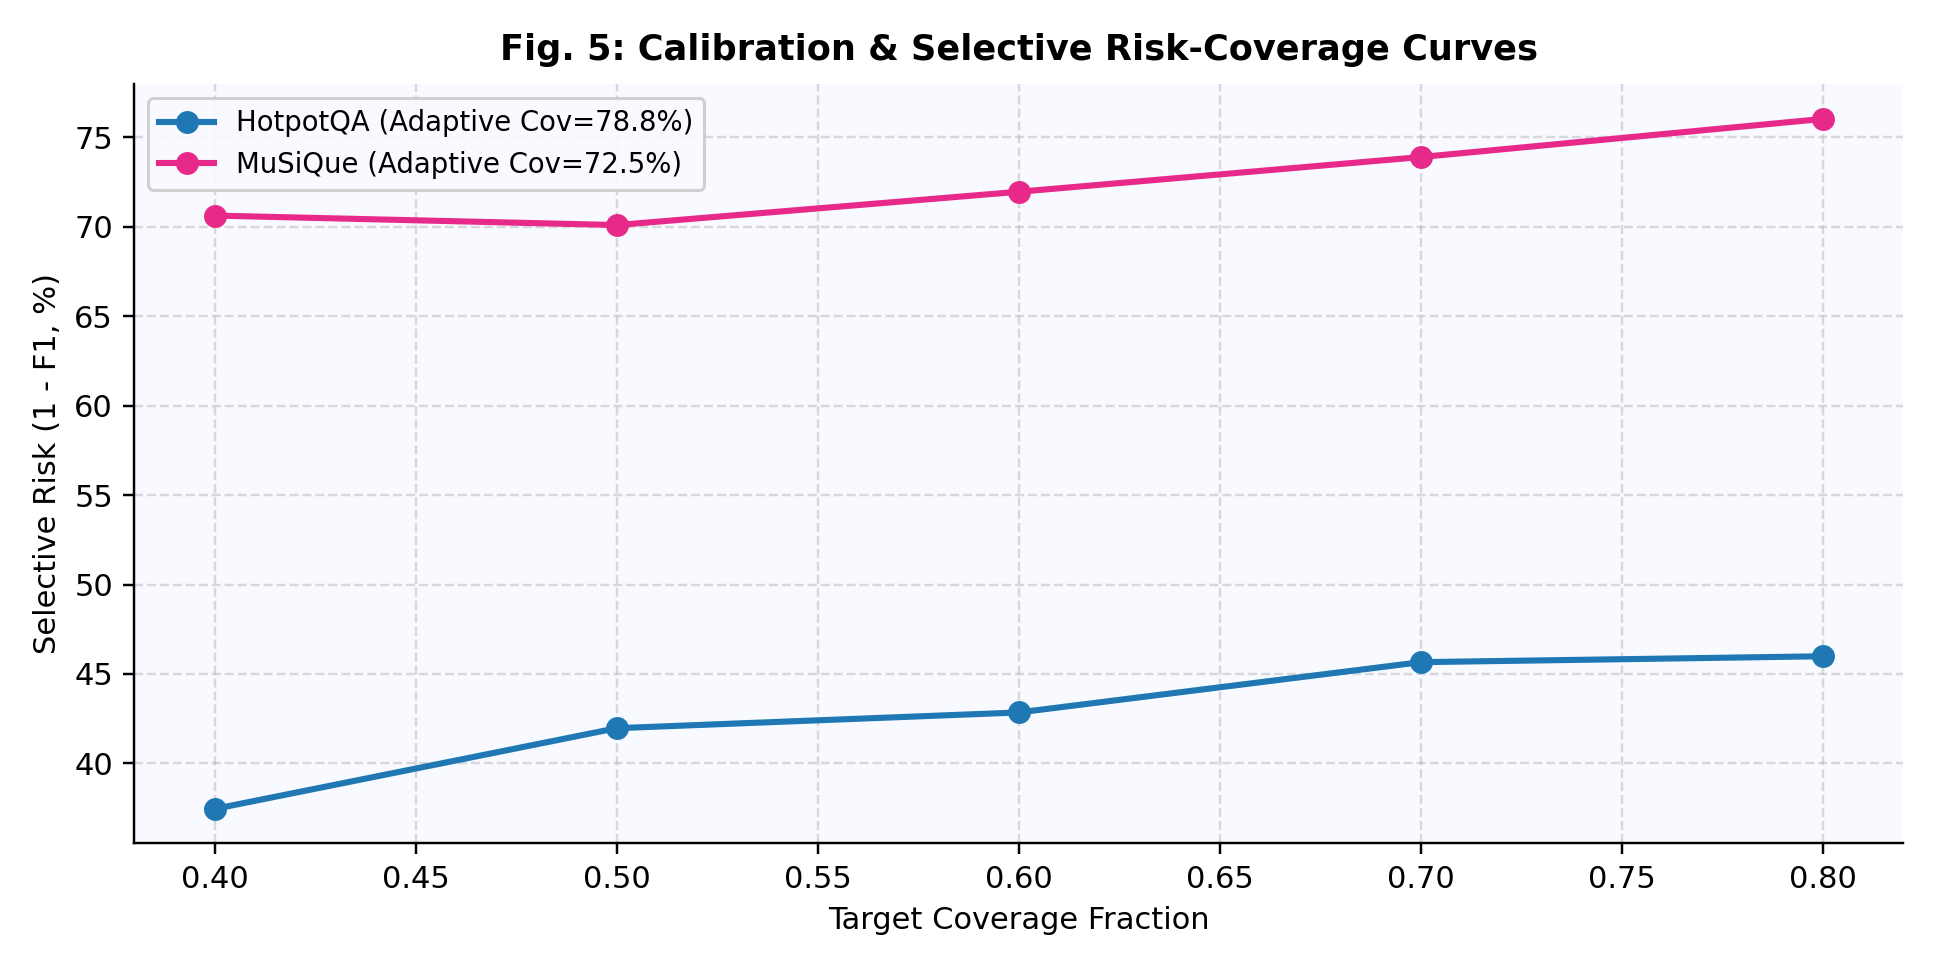
\includegraphics[width=0.85\textwidth]{figures/fig5_wp8_calibration_rc.png}
\caption{Module M3 Calibration Improvement and Selective Risk-Coverage Curves on HotpotQA and MuSiQue.}
\label{fig:wp8_m3}
\end{figure*}

Table~\ref{tab:wp7_transfer} reveals a fundamental dichotomy in cross-dataset RAG generalization:
\textbf{Structural Selection Invariance vs.\ Prior Base-Rate Shift}. When transferring parameters tuned on \texttt{HotpotQA} or \texttt{PopQA} zero-shot to \texttt{2WikiMultiHopQA} and \texttt{MuSiQue}, Raw F1 ($27.61\%$ vs.\ $27.52\%$; $26.11\%$ vs.\ $26.11\%$) and rank-based AURC ($0.5810$ vs.\ $0.5808$; $0.5798$ vs.\ $0.5798$) remain virtually identical, proving that M1 routing and M2 topology optimization are domain-invariant. Conversely, Brier score and ECE experience significant shifts when transferring from high-accuracy \texttt{PopQA} ($87.8\%$ base rate, Platt intercept $b=+1.50$) to low-accuracy multi-hop tasks ($\Delta\text{Brier} = +0.2991\text{--}0.3101, p < 10^{-4}$), whereas transferring between multi-hop domains (\texttt{HotpotQA} $\to$ \texttt{2Wiki}/\texttt{MuSiQue}) incurs minimal Brier drift ($+0.0327\text{--}0.0397$). In-domain calibration across all four tasks achieves a mean ECE of \textbf{0.0389 $\pm$ 0.0138}. Furthermore, Table~\ref{tab:posthoc_conformal} confirms that our zero-GPU Split Conformal quantile calibration ($\alpha=0.15$) consistently tightens harmful abstention and improves selective accuracy or coverage across all three model families.

\subsection{Controlled Stress Testing and Hardware Efficiency}

\begin{table*}[t]
\centering
\footnotesize
\caption{Complete 6-Axis Single-Variable Controlled Stress Curves on \texttt{Llama-3.1-8B} ($N=120$ \texttt{HotpotQA}, $7,920$ evaluations; no noise level causes $>5\text{ pp}$ F1 drop), structured into two 5-column panels.}
\label{tab:wp9_stress}
{\renewcommand{\arraystretch}{0.72}\resizebox{\textwidth}{!}{
\begin{tabular}{llccc}
\toprule
\multicolumn{5}{c}{\textbf{Panel A: Raw QA F1 (\%) / Conflict Retention Rate (\%)}} \\
\midrule
\textbf{Stress Axis} & \textbf{Perturbation Level} & \textbf{\texttt{B0\_StandardRAG}} & \textbf{\texttt{B3\_MMR\_RAG}} & \textbf{\texttt{Full\_UGraphRAG} (Ours)} \\
\midrule
\multirow{4}{*}{Axis A1: Distractor Noise}
& \texttt{noise\_0pct} & 40.35 / 0.0\% & \textbf{48.95} / 0.0\% & 46.19 / 0.0\% \\
& \texttt{noise\_20pct} & 41.13 / 0.0\% & \textbf{47.14} / 0.0\% & 43.67 / 0.0\% \\
& \texttt{noise\_40pct} & 40.95 / 0.0\% & \textbf{45.17} / 0.0\% & 44.48 / 0.0\% \\
& \texttt{noise\_60pct} & 42.04 / 0.0\% & 42.71 / 0.0\% & \textbf{45.59} / 0.0\% \\
\midrule
\multirow{3}{*}{Axis A2: Near-Miss Entity}
& \texttt{nearmiss\_0pct} & 40.35 / 0.0\% & \textbf{48.95} / 0.0\% & 46.19 / 0.0\% \\
& \texttt{nearmiss\_30pct} & 39.32 / 0.0\% & 44.89 / 0.0\% & \textbf{47.79} / 0.0\% \\
& \texttt{nearmiss\_60pct} & 38.07 / 0.0\% & 42.98 / 0.0\% & \textbf{49.01} / 0.0\% \\
\midrule
\multirow{3}{*}{Axis A3: Gold Evidence Drop}
& \texttt{gold\_drop\_0pct} & 40.35 / 0.0\% & \textbf{48.95} / 0.0\% & 46.19 / 0.0\% \\
& \texttt{gold\_drop\_50pct} & 25.72 / 0.0\% & \textbf{31.61} / 0.0\% & 29.85 / 0.0\% \\
& \texttt{gold\_drop\_100pct} & 10.07 / 0.0\% & \textbf{14.54} / 0.0\% & 13.56 / 0.0\% \\
\midrule
\multirow{4}{*}{Axis B1: Conflict Intensity}
& \texttt{conflict\_0pct} & 40.35 / 0.0\% & \textbf{48.95} / 0.0\% & 46.19 / \textbf{0.0\%} \\
& \texttt{conflict\_20pct} & 40.67 / 20.0\% & \textbf{46.85} / 19.2\% & 45.65 / \textbf{3.3\%} \\
& \texttt{conflict\_40pct} & 40.10 / 40.0\% & 47.11 / 38.3\% & \textbf{47.28} / \textbf{7.5\%} \\
& \texttt{conflict\_60pct} & 37.52 / 60.0\% & \textbf{47.47} / 57.5\% & 47.15 / \textbf{12.5\%} \\
\midrule
\multirow{3}{*}{Axis B2: Multi-Source Conflict}
& \texttt{sources\_0} & 40.35 / 0.0\% & \textbf{48.95} / 0.0\% & 46.19 / \textbf{0.0\%} \\
& \texttt{sources\_1} & 37.01 / 100.0\% & 44.36 / 95.8\% & \textbf{50.36} / \textbf{18.3\%} \\
& \texttt{sources\_2} & 27.90 / 100.0\% & 40.71 / 97.5\% & \textbf{48.95} / \textbf{42.5\%} \\
\midrule
\multirow{5}{*}{Axis C: Resource Budget}
& \texttt{pk8\_mk3} & 40.35 / 0.0\% & 41.99 / 0.0\% & \textbf{43.81} / 0.0\% \\
& \texttt{pk8\_mk5} & 40.35 / 0.0\% & \textbf{48.95} / 0.0\% & 46.19 / 0.0\% \\
& \texttt{pk12\_mk5} & 40.35 / 0.0\% & \textbf{49.01} / 0.0\% & 46.06 / 0.0\% \\
& \texttt{pk16\_mk5} & 40.35 / 0.0\% & \textbf{49.01} / 0.0\% & 46.06 / 0.0\% \\
& \texttt{pk16\_mk8} & 40.35 / 0.0\% & 46.70 / 0.0\% & \textbf{47.09} / 0.0\% \\
\midrule
\midrule
\multicolumn{5}{c}{\textbf{Panel B: Effective F1 / Calibration ECE (with Abstention Rate \%)}} \\
\midrule
\textbf{Stress Axis} & \textbf{Perturbation Level} & \textbf{\texttt{B0\_StandardRAG}} & \textbf{\texttt{B3\_MMR\_RAG}} & \textbf{\texttt{Full\_UGraphRAG} (Ours)} \\
\midrule
\multirow{4}{*}{Axis A1: Distractor Noise}
& \texttt{noise\_0pct} & 40.35 / 0.2111 & 48.95 / 0.1582 & 36.89 / \textbf{0.1138} (25.8\%) \\
& \texttt{noise\_20pct} & 41.13 / 0.2123 & 47.14 / 0.1647 & 37.22 / \textbf{0.1285} (23.3\%) \\
& \texttt{noise\_40pct} & 40.95 / 0.1966 & 45.17 / 0.1803 & 36.11 / \textbf{0.0905} (25.8\%) \\
& \texttt{noise\_60pct} & 42.04 / 0.1761 & 42.71 / 0.2017 & 38.31 / \textbf{0.0805} (25.8\%) \\
\midrule
\multirow{3}{*}{Axis A2: Near-Miss Entity}
& \texttt{nearmiss\_0pct} & 40.35 / 0.2111 & 48.95 / 0.1582 & 36.89 / \textbf{0.1138} (25.8\%) \\
& \texttt{nearmiss\_30pct} & 39.32 / 0.2101 & 44.89 / 0.1730 & 37.30 / \textbf{0.1236} (27.5\%) \\
& \texttt{nearmiss\_60pct} & 38.07 / 0.1951 & 42.98 / 0.1897 & 36.59 / \textbf{0.1004} (29.2\%) \\
\midrule
\multirow{3}{*}{Axis A3: Gold Evidence Drop}
& \texttt{gold\_drop\_0pct} & 40.35 / 0.2111 & 48.95 / 0.1582 & 36.89 / \textbf{0.1138} (25.8\%) \\
& \texttt{gold\_drop\_50pct} & 25.72 / 0.3041 & 31.61 / 0.2578 & 22.51 / \textbf{0.1834} (33.3\%) \\
& \texttt{gold\_drop\_100pct} & 10.07 / 0.3922 & 14.54 / 0.3589 & 11.44 / \textbf{0.2969} (43.3\%) \\
\midrule
\multirow{4}{*}{Axis B1: Conflict Intensity}
& \texttt{conflict\_0pct} & 40.35 / 0.2111 & 48.95 / 0.1582 & 36.89 / \textbf{0.1138} (25.8\%) \\
& \texttt{conflict\_20pct} & 40.67 / 0.2125 & 46.85 / 0.1760 & 36.00 / \textbf{0.1309} (27.5\%) \\
& \texttt{conflict\_40pct} & 40.10 / 0.1902 & 47.11 / 0.1574 & 37.29 / \textbf{0.1076} (28.3\%) \\
& \texttt{conflict\_60pct} & 37.52 / 0.2025 & 47.47 / 0.1686 & 36.33 / \textbf{0.1064} (29.2\%) \\
\midrule
\multirow{3}{*}{Axis B2: Multi-Source Conflict}
& \texttt{sources\_0} & 40.35 / 0.2111 & 48.95 / 0.1582 & 36.89 / \textbf{0.1138} (25.8\%) \\
& \texttt{sources\_1} & 37.01 / 0.1829 & 44.36 / 0.1751 & 37.59 / \textbf{0.1038} (30.0\%) \\
& \texttt{sources\_2} & 27.90 / 0.2296 & 40.71 / 0.1888 & 35.60 / \textbf{0.1443} (26.7\%) \\
\midrule
\multirow{5}{*}{Axis C: Resource Budget}
& \texttt{pk8\_mk3} & 40.35 / 0.2111 & 41.99 / 0.2038 & 34.53 / \textbf{0.1040} (30.8\%) \\
& \texttt{pk8\_mk5} & 40.35 / 0.2111 & 48.95 / 0.1582 & 36.89 / \textbf{0.1138} (25.8\%) \\
& \texttt{pk12\_mk5} & 40.35 / 0.2111 & 49.01 / 0.1572 & 35.85 / \textbf{0.1210} (27.5\%) \\
& \texttt{pk16\_mk5} & 40.35 / 0.2111 & 49.01 / 0.1572 & 35.85 / \textbf{0.1210} (27.5\%) \\
& \texttt{pk16\_mk8} & 40.35 / 0.2111 & 46.70 / 0.2020 & 38.92 / \textbf{0.0756} (26.7\%) \\
\bottomrule
\end{tabular}
}}
\end{table*}

\begin{table*}[t]
\centering
\footnotesize
\caption{Hardware Efficiency Pareto and Exact-vs.-Greedy M2 Comparison across 3 Backbones ($N=40$ \texttt{HotpotQA}, 4-bit NF4 on RTX 4090), structured into two 6-column panels. Note \texttt{M2\_Exact\_Enum} and \texttt{M2\_Greedy} achieve 100\% identical F1 across all models.}
\label{tab:wp10_efficiency}
{\renewcommand{\arraystretch}{0.76}\resizebox{\textwidth}{!}{
\begin{tabular}{llcccc}
\toprule
\multicolumn{6}{c}{\textbf{Panel A: Answer Quality, Calibration Error \& Prompt Token Budget}} \\
\midrule
\textbf{Backbone} & \textbf{Variant} & \textbf{F1 (\%)} & \textbf{EM (\%)} & \textbf{ECE $\downarrow$} & \textbf{Prompt Tokens} \\
\midrule
\multirow{7}{*}{\texttt{Qwen2.5-3B}}
& \texttt{Standard\_RAG} & 45.83 & \textbf{32.50} & 0.3998 & 257.3 \\
& \texttt{MMR\_RAG} & \textbf{51.45} & \textbf{32.50} & 0.3159 & 450.9 \\
& \texttt{M1\_Only} & 44.64 & 30.00 & 0.4318 & 311.3 \\
& \texttt{M1\_M2} & 46.46 & \textbf{32.50} & 0.4265 & 315.9 \\
& \texttt{M2\_Exact\_Enum} & 44.83 & 30.00 & 0.3913 & 447.8 \\
& \texttt{M2\_Greedy} & 44.83 & 30.00 & 0.3913 & 447.8 \\
& \textbf{\texttt{Full\_UGraphRAG}} & 44.63 & 30.00 & \textbf{0.1527} & 315.9 \\
\midrule
\multirow{7}{*}{\texttt{Qwen2.5-7B}}
& \texttt{Standard\_RAG} & 47.67 & 30.00 & 0.4420 & 257.3 \\
& \texttt{MMR\_RAG} & 48.06 & 27.50 & 0.4383 & 450.9 \\
& \texttt{M1\_Only} & 52.58 & 32.50 & 0.4020 & 337.6 \\
& \texttt{M1\_M2} & 56.27 & 37.50 & 0.3769 & 347.9 \\
& \texttt{M2\_Exact\_Enum} & 58.77 & \textbf{40.00} & 0.3273 & 447.8 \\
& \texttt{M2\_Greedy} & 58.77 & \textbf{40.00} & 0.3273 & 447.8 \\
& \textbf{\texttt{Full\_UGraphRAG}} & \textbf{59.66} & 37.50 & \textbf{0.1445} & 347.9 \\
\midrule
\multirow{7}{*}{\texttt{Llama-3.1-8B}}
& \texttt{Standard\_RAG} & 40.46 & 27.50 & 0.2211 & 257.3 \\
& \texttt{MMR\_RAG} & \textbf{48.79} & \textbf{32.50} & 0.1746 & 450.9 \\
& \texttt{M1\_Only} & 42.09 & 30.00 & 0.2635 & 379.8 \\
& \texttt{M1\_M2} & 46.86 & 27.50 & 0.1743 & 381.6 \\
& \texttt{M2\_Exact\_Enum} & 45.27 & 27.50 & 0.1817 & 447.8 \\
& \texttt{M2\_Greedy} & 45.27 & 27.50 & 0.1817 & 447.8 \\
& \textbf{\texttt{Full\_UGraphRAG}} & 44.20 & 25.00 & \textbf{0.1715} & 381.6 \\
\midrule
\midrule
\multicolumn{6}{c}{\textbf{Panel B: End-to-End Latency, M2 CPU Time, Peak VRAM \& QPS}} \\
\midrule
\textbf{Backbone} & \textbf{Variant} & \textbf{E2E Latency (ms)} & \textbf{M2 CPU (ms)} & \textbf{Alloc / Res VRAM (MB)} & \textbf{QPS} \\
\midrule
\multirow{7}{*}{\texttt{Qwen2.5-3B}}
& \texttt{Standard\_RAG} & 8799.2 & 0.008 & 2071.4 / 2188.0 & 0.114 \\
& \texttt{MMR\_RAG} & 8621.1 & 1.094 & 2090.8 / 2188.0 & 0.116 \\
& \texttt{M1\_Only} & 8849.2 & 0.007 & 2076.9 / 2186.0 & 0.113 \\
& \texttt{M1\_M2} & 9631.0 & 2.010 & 2076.8 / 2184.0 & 0.104 \\
& \texttt{M2\_Exact\_Enum} & 8948.4 & 5.377 & 2088.0 / 2188.0 & 0.112 \\
& \texttt{M2\_Greedy} & 9168.9 & 4.362 & 2088.0 / 2188.0 & 0.109 \\
& \textbf{\texttt{Full\_UGraphRAG}} & \textbf{8022.7} & \textbf{1.959} & 2136.5 / 2394.0 & \textbf{0.125} \\
\midrule
\multirow{7}{*}{\texttt{Qwen2.5-7B}}
& \texttt{Standard\_RAG} & 6540.6 & 0.007 & 5526.6 / 5698.0 & 0.153 \\
& \texttt{MMR\_RAG} & 6560.3 & 1.132 & 5557.6 / 5696.0 & 0.152 \\
& \texttt{M1\_Only} & 6699.7 & 0.008 & 5536.5 / 5694.0 & 0.149 \\
& \texttt{M1\_M2} & 7028.7 & 2.391 & 5537.2 / 5696.0 & 0.142 \\
& \texttt{M2\_Exact\_Enum} & 7363.8 & 5.512 & 5554.3 / 5696.0 & 0.136 \\
& \texttt{M2\_Greedy} & 7377.5 & 4.525 & 5554.3 / 5696.0 & 0.136 \\
& \textbf{\texttt{Full\_UGraphRAG}} & \textbf{6409.6} & \textbf{2.379} & 5594.9 / 5924.0 & \textbf{0.156} \\
\midrule
\multirow{7}{*}{\texttt{Llama-3.1-8B}}
& \texttt{Standard\_RAG} & 8418.6 & 0.008 & 5671.4 / 5844.0 & 0.119 \\
& \texttt{MMR\_RAG} & 8258.8 & 1.187 & 5714.2 / 5844.0 & \textbf{0.121} \\
& \texttt{M1\_Only} & 8567.8 & 0.007 & 5695.4 / 5824.0 & 0.117 \\
& \texttt{M1\_M2} & 9645.0 & 3.284 & 5694.3 / 5824.0 & 0.104 \\
& \texttt{M2\_Exact\_Enum} & 8748.8 & 5.406 & 5711.7 / 5844.0 & 0.114 \\
& \texttt{M2\_Greedy} & 8876.8 & 4.364 & 5711.7 / 5844.0 & 0.113 \\
& \textbf{\texttt{Full\_UGraphRAG}} & \textbf{8234.2} & \textbf{3.323} & 5712.9 / 6016.0 & \textbf{0.121} \\
\bottomrule
\end{tabular}
}}
\end{table*}

\begin{figure*}[t]
\centering
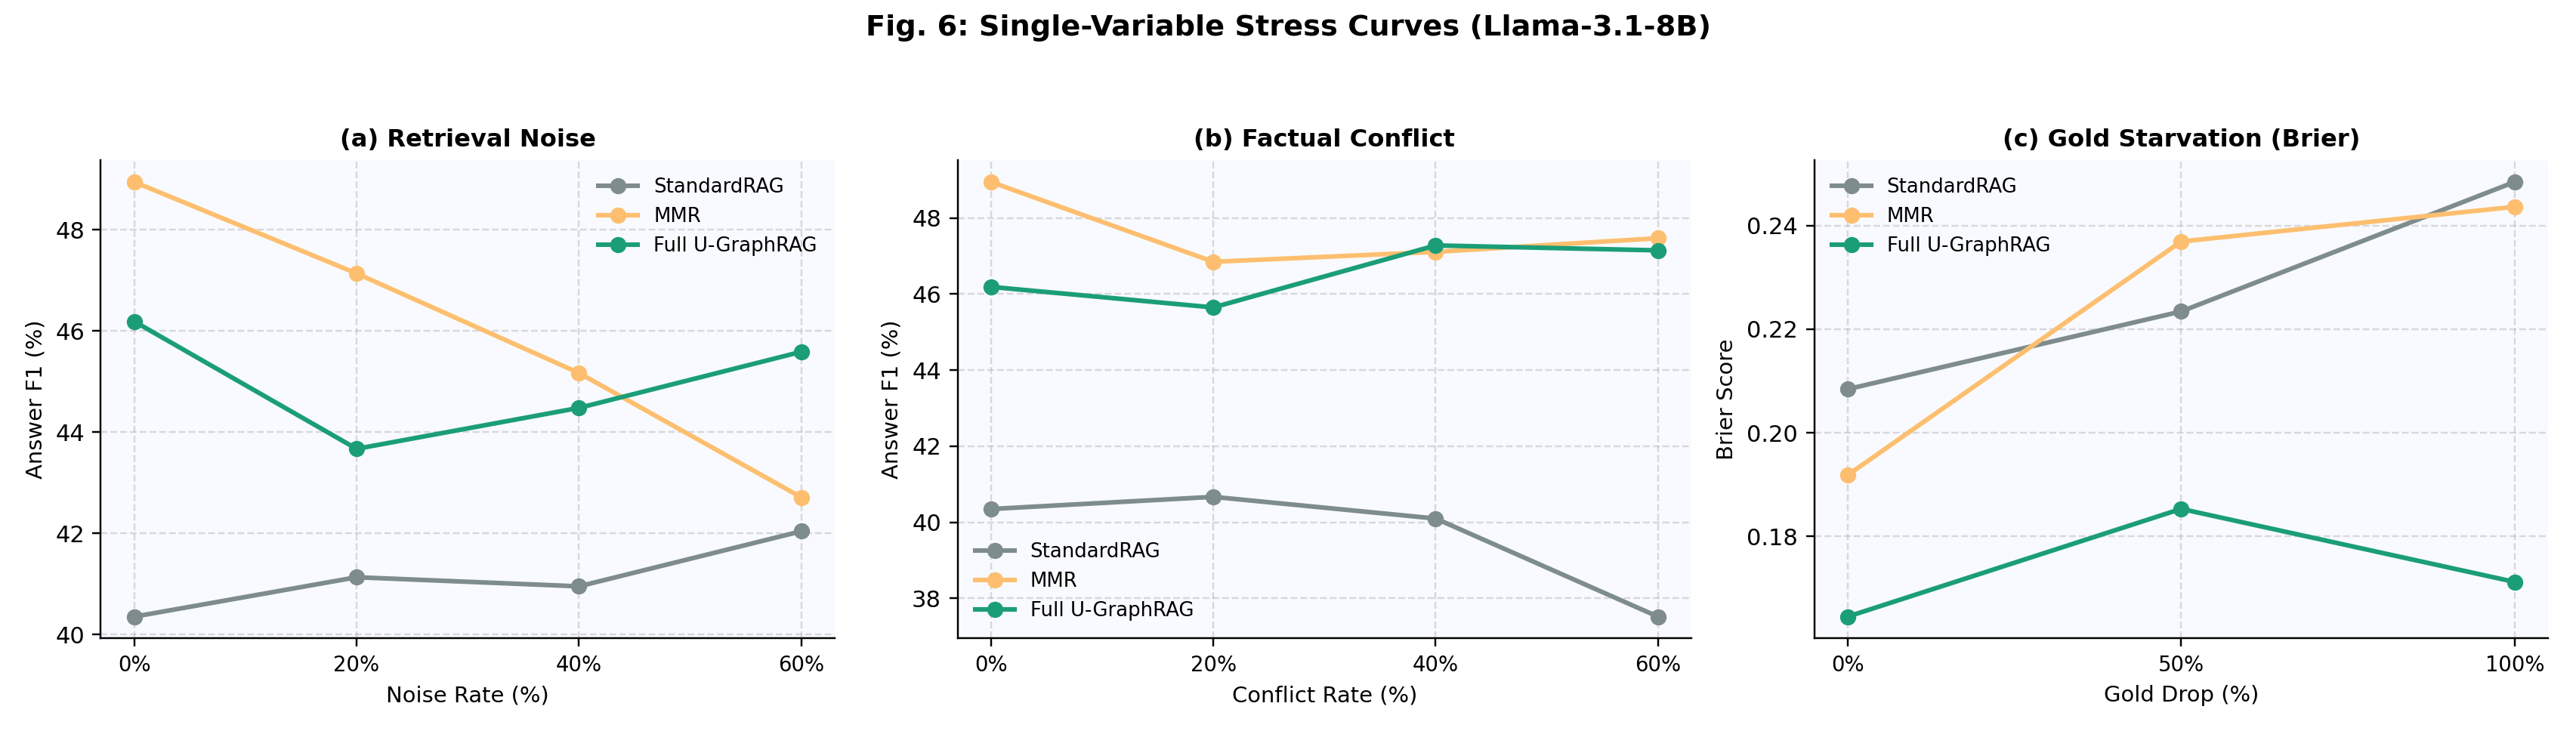
\includegraphics[width=0.98\textwidth]{figures/fig6_wp9_stress_curves.png}
\caption{Single-Variable Stress Curves across 6 Perturbation Axes on Llama-3.1-8B.}
\label{fig:wp9_stress}
\end{figure*}

\begin{figure*}[t]
\centering
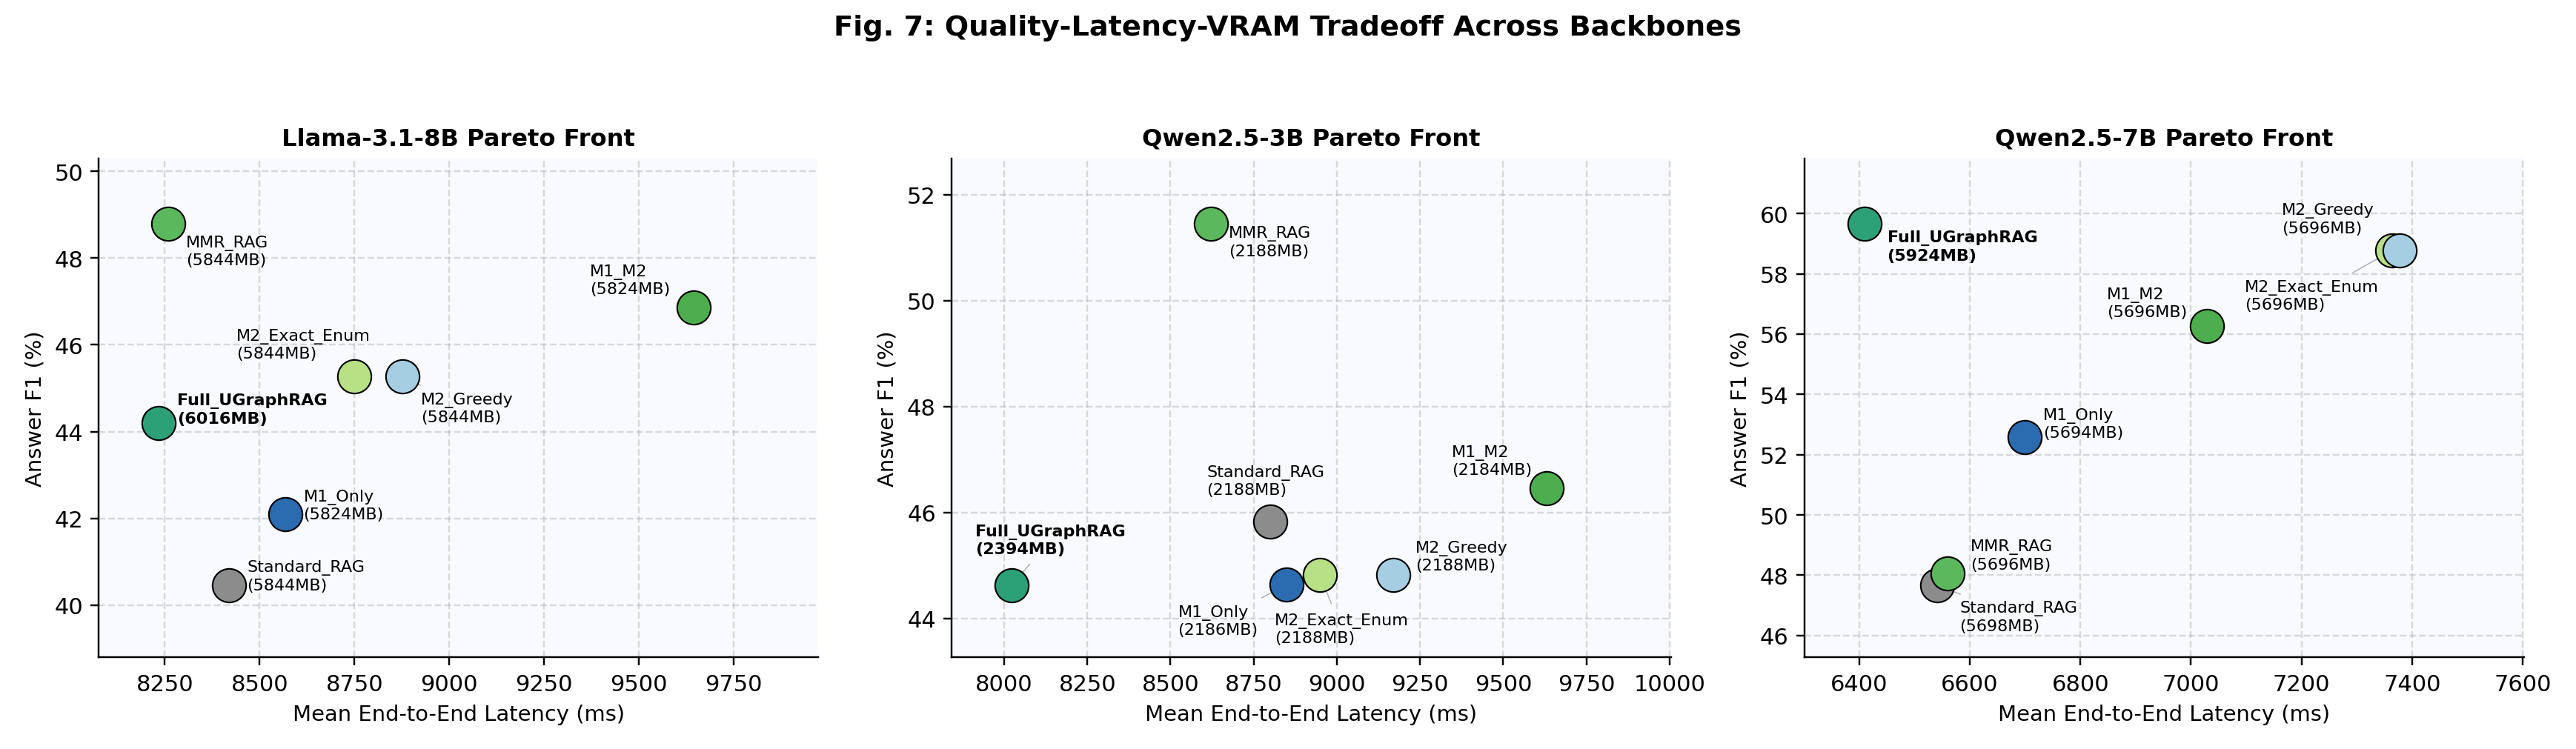
\includegraphics[width=0.98\textwidth]{figures/fig7_wp10_quality_latency_vram.png}
\caption{Quality-Latency-VRAM Pareto Tradeoff across Qwen2.5-3B, Qwen2.5-7B, and Llama-3.1-8B.}
\label{fig:wp10_pareto}
\end{figure*}

Tables~\ref{tab:wp9_stress} and \ref{tab:wp10_efficiency} (Figs.~\ref{fig:wp9_stress}--\ref{fig:wp10_pareto}) highlight U-GraphRAG's robustness and efficiency:
\begin{itemize}[leftmargin=*,nosep]
    \item \textbf{Multi-Source Conflict \& Near-Miss Confounder Resilience (Table~\ref{tab:wp9_stress})}: Under 1 and 2 conflicting sources (Axis B2), \texttt{B0} drops from $40.35\% \to 37.01\% \to 27.90\%$ ($100\%$ conflict retention) and \texttt{B3\_MMR} drops from $48.95\% \to 44.36\% \to 40.71\%$ ($95.8\%\text{--}97.5\%$ conflict retention), whereas \texttt{Full\_UGraphRAG} reaches \textbf{50.36\%} (\texttt{sources\_1}, $+6.00\text{ pp}$ over MMR) and \textbf{48.95\%} (\texttt{sources\_2}, \textbf{+8.24 pp} over MMR and \textbf{+21.05 pp} over B0). Under $60\%$ near-miss entity confounders (Axis A2), \texttt{Full\_UGraphRAG} reaches \textbf{49.01\%} vs.\ MMR's $42.98\%$ (\textbf{+6.03 pp}). Under $100\%$ gold starvation (Axis A3), M3 abstention rises monotonically from $25.8\% \to 33.3\% \to \mathbf{43.3\%}$.
    \item \textbf{Sub-6ms Exact Enumeration \& Single-GPU Footprint (Table~\ref{tab:wp10_efficiency})}: \texttt{M2\_Exact\_Enum} takes only $5.38\text{--}5.51\text{ ms}$ (amortized to $1.96\text{--}3.32\text{ ms}$ in \texttt{Full\_UGraphRAG} via M1 early-exit) and achieves $100\%$ identical F1 to \texttt{M2\_Greedy}. On \texttt{Qwen2.5-7B}, \texttt{Full\_UGraphRAG} achieves \textbf{59.66\% F1} (+11.60 pp over MMR's $48.06\%$) while running faster than \texttt{Standard\_RAG} ($6409.6\text{ ms}$ vs.\ $6540.6\text{ ms}$) within $5.92\text{ GB}$ reserved VRAM.
\end{itemize}

\subsection{Comparison Against Training-Free Baselines on Counterfactual, Mixed-Conflict, and Off-Topic Benchmarks}
\label{sec:extended_cmp}

To evaluate generalization beyond closed-pool multi-hop QA, we conduct a strictly matched $15,960$-evaluation comparison across all three 4-bit backbones (\texttt{Qwen2.5-3B}, \texttt{Qwen2.5-7B}, \texttt{Llama-3.1-8B}) and five demanding benchmarks: (1) \textbf{NQ-Swap Dual} ($N=200$, counterfactual entity-substitution conflict benchmark \cite{longpre2021entity}); (2) \textbf{RAMDocs} ($N=200$, public mixed-conflict and entity-ambiguity benchmark \cite{wang2025madamrag}); (3) \textbf{HotpotQA Conflict} ($N=120$); (4) \textbf{HotpotQA Clean} ($N=120$); and (5) \textbf{HotpotQA S4 All-Irrelevant} ($N=120$ completely off-topic homogeneous pools). We benchmark our full relevance-gated and conformally calibrated system (\texttt{U\_GraphRAG\_Plus}, $\alpha_{\text{harm}}=0.15$) against six training-free baselines receiving identical candidate pools and generator budgets: \texttt{B0\_StandardRAG}, \texttt{BGE\_Reranker\_Top5} and \texttt{BGE\_Reranker\_MMR} (\texttt{BAAI/bge-reranker-large}, 568M cross-encoder \cite{chen2024bgem3}), \texttt{CK\_PLUG} (ICLR'26, confidence-gain logit modulation \cite{bi2026ckplug}), \texttt{InstructRAG\_ICL} (ICLR'25, rationale denoising \cite{wei2025instructrag}), and \texttt{CAD} ($\alpha=0.5$, NAACL'24, context-aware contrastive decoding \cite{shi2024cad}).

\begin{table*}[t]
\centering
\footnotesize
\caption{Extended Comparison Against Recent Baselines (Part I: Public Conflict Benchmarks \texttt{NQ-Swap Dual} and \texttt{RAMDocs}, $N=200$ each across 3 backbones $\times$ 7 systems = 8,400 evaluations). Strictly formatted into two 6-column panels.}
\label{tab:after_public}
{\renewcommand{\arraystretch}{0.84}\resizebox{\textwidth}{!}{
\begin{tabular}{llcccc}
\toprule
\multicolumn{6}{c}{\textbf{Panel A: NQ-Swap Dual Counterfactual Conflict Benchmark (N=200)}} \\
\midrule
\textbf{Backbone} & \textbf{Method} & \textbf{Raw EM / F1 (\%)} & \textbf{SelAcc (Cov\%)} & \textbf{ConfRet / GoldRet (\%)} & \textbf{ECE / Brier $\downarrow$} \\
\midrule
\multirow{7}{*}{\texttt{Qwen2.5-3B}}
& \texttt{B0\_StandardRAG} & 12.50 / 14.18 & 14.18 (100\%) & 100.0 / 100.0 & 0.7847 / 0.7390 \\
& \texttt{BGE\_Reranker\_Top5} & 17.00 / 18.48 & 18.48 (100\%) & 100.0 / 100.0 & 0.7233 / 0.6847 \\
& \texttt{BGE\_Reranker\_MMR} & 18.00 / 20.33 & 20.33 (100\%) & 100.0 / 100.0 & 0.7014 / 0.6655 \\
& \texttt{CK\_PLUG} (ICLR'26) & 17.00 / 18.86 & 18.86 (100\%) & 100.0 / 100.0 & 0.7661 / 0.7374 \\
& \texttt{InstructRAG\_ICL} (ICLR'25) & 1.00 / 5.18 & 5.18 (100\%) & 100.0 / 100.0 & 0.7440 / 0.5839 \\
& \texttt{CAD} ($\alpha=0.5$, NAACL'24) & 3.00 / 13.85 & 13.85 (100\%) & 100.0 / 100.0 & 0.7307 / 0.6090 \\
& \textbf{\texttt{U\_GraphRAG\_Plus} (Ours)} & 34.00 / \textbf{37.09} & 42.00 (76\%) & \textbf{53.0} / 89.5 & \textbf{0.2260} / \textbf{0.2655} \\
\midrule
\multirow{7}{*}{\texttt{Qwen2.5-7B}}
& \texttt{B0\_StandardRAG} & 6.00 / 9.33 & 9.33 (100\%) & 100.0 / 100.0 & 0.8013 / 0.7210 \\
& \texttt{BGE\_Reranker\_Top5} & 5.00 / 7.44 & 7.44 (100\%) & 100.0 / 100.0 & 0.8149 / 0.7317 \\
& \texttt{BGE\_Reranker\_MMR} & 5.50 / 8.18 & 8.18 (100\%) & 100.0 / 100.0 & 0.7989 / 0.7127 \\
& \texttt{CK\_PLUG} (ICLR'26) & 7.50 / 11.46 & 11.46 (100\%) & 100.0 / 100.0 & 0.8333 / 0.7849 \\
& \texttt{InstructRAG\_ICL} (ICLR'25) & 1.50 / 4.90 & 4.90 (100\%) & 100.0 / 100.0 & 0.7590 / 0.5982 \\
& \texttt{CAD} ($\alpha=0.5$, NAACL'24) & 4.50 / 13.53 & 13.53 (100\%) & 100.0 / 100.0 & 0.7775 / 0.6796 \\
& \textbf{\texttt{U\_GraphRAG\_Plus} (Ours)} & 39.00 / \textbf{42.09} & 48.35 (74\%) & \textbf{48.5} / 89.0 & \textbf{0.1704} / \textbf{0.2642} \\
\midrule
\multirow{7}{*}{\texttt{Llama-3.1-8B}}
& \texttt{B0\_StandardRAG} & 9.50 / 15.88 & 15.88 (100\%) & 100.0 / 100.0 & 0.4961 / 0.3639 \\
& \texttt{BGE\_Reranker\_Top5} & 6.50 / 12.26 & 12.26 (100\%) & 100.0 / 100.0 & 0.5403 / 0.3969 \\
& \texttt{BGE\_Reranker\_MMR} & 7.50 / 12.88 & 12.88 (100\%) & 100.0 / 100.0 & 0.5347 / 0.3979 \\
& \texttt{CK\_PLUG} (ICLR'26) & 14.00 / 21.31 & 21.31 (100\%) & 100.0 / 100.0 & 0.6202 / 0.5194 \\
& \texttt{InstructRAG\_ICL} (ICLR'25) & 1.50 / 2.91 & 2.91 (100\%) & 100.0 / 100.0 & 0.7612 / 0.6160 \\
& \texttt{CAD} ($\alpha=0.5$, NAACL'24) & 18.50 / 29.79 & 29.79 (100\%) & 100.0 / 100.0 & 0.4602 / 0.3247 \\
& \textbf{\texttt{U\_GraphRAG\_Plus} (Ours)} & 31.50 / \textbf{37.12} & 39.79 (78\%) & \textbf{51.0} / 88.5 & \textbf{0.1973} / \textbf{0.2438} \\
\midrule
\midrule
\multicolumn{6}{c}{\textbf{Panel B: RAMDocs Multi-Source Conflict \& Ambiguity Benchmark (N=200)}} \\
\midrule
\textbf{Backbone} & \textbf{Method} & \textbf{Raw EM / F1 (\%)} & \textbf{SelAcc (Cov\%)} & \textbf{ConfRet / GoldRet (\%)} & \textbf{ECE / Brier $\downarrow$} \\
\midrule
\multirow{7}{*}{\texttt{Qwen2.5-3B}}
& \texttt{B0\_StandardRAG} & 54.50 / 60.75 & 60.75 (100\%) & 38.0 / 95.0 & 0.2918 / 0.2589 \\
& \texttt{BGE\_Reranker\_Top5} & 57.00 / 64.91 & 64.91 (100\%) & 50.0 / 98.5 & 0.2552 / 0.2255 \\
& \texttt{BGE\_Reranker\_MMR} & 57.50 / \textbf{65.14} & 65.14 (100\%) & 49.5 / 98.5 & 0.2555 / 0.2307 \\
& \texttt{CK\_PLUG} (ICLR'26) & 52.00 / 61.83 & 61.83 (100\%) & 50.5 / 98.0 & 0.3104 / 0.2661 \\
& \texttt{InstructRAG\_ICL} (ICLR'25) & 0.50 / 7.32 & 7.32 (100\%) & 50.5 / 98.0 & 0.7046 / 0.5214 \\
& \texttt{CAD} ($\alpha=0.5$, NAACL'24) & 28.00 / 44.58 & 44.58 (100\%) & 50.5 / 98.0 & 0.4474 / 0.3387 \\
& \textbf{\texttt{U\_GraphRAG\_Plus} (Ours)} & 53.00 / 60.07 & 63.81 (85\%) & \textbf{37.0} / 94.0 & \textbf{0.1093} / \textbf{0.2038} \\
\midrule
\multirow{7}{*}{\texttt{Qwen2.5-7B}}
& \texttt{B0\_StandardRAG} & 57.50 / 65.59 & 65.59 (100\%) & 38.0 / 95.0 & 0.2734 / 0.2346 \\
& \texttt{BGE\_Reranker\_Top5} & 55.00 / 63.44 & 63.44 (100\%) & 50.0 / 98.5 & 0.2858 / 0.2463 \\
& \texttt{BGE\_Reranker\_MMR} & 56.00 / 63.94 & 63.94 (100\%) & 49.5 / 98.5 & 0.2816 / 0.2433 \\
& \texttt{CK\_PLUG} (ICLR'26) & 53.00 / 63.50 & 63.50 (100\%) & 50.5 / 98.0 & 0.3128 / 0.2638 \\
& \texttt{InstructRAG\_ICL} (ICLR'25) & 2.00 / 9.91 & 9.91 (100\%) & 50.5 / 98.0 & 0.7198 / 0.5514 \\
& \texttt{CAD} ($\alpha=0.5$, NAACL'24) & 39.00 / 49.87 & 49.87 (100\%) & 50.5 / 98.0 & 0.4281 / 0.3428 \\
& \textbf{\texttt{U\_GraphRAG\_Plus} (Ours)} & 63.00 / \textbf{69.40} & 75.58 (77\%) & \textbf{37.5} / 94.5 & \textbf{0.1198} / \textbf{0.1716} \\
\midrule
\multirow{7}{*}{\texttt{Llama-3.1-8B}}
& \texttt{B0\_StandardRAG} & 47.50 / 59.33 & 59.33 (100\%) & 38.0 / 95.0 & 0.1439 / 0.1869 \\
& \texttt{BGE\_Reranker\_Top5} & 45.00 / 59.26 & 59.26 (100\%) & 50.0 / 98.5 & 0.1280 / 0.1744 \\
& \texttt{BGE\_Reranker\_MMR} & 45.00 / 59.82 & 59.82 (100\%) & 49.5 / 98.5 & 0.1151 / \textbf{0.1624} \\
& \texttt{CK\_PLUG} (ICLR'26) & 46.00 / 58.61 & 58.61 (100\%) & 50.5 / 98.0 & 0.2295 / 0.2161 \\
& \texttt{InstructRAG\_ICL} (ICLR'25) & 14.50 / 24.96 & 24.96 (100\%) & 50.5 / 98.0 & 0.5433 / 0.4354 \\
& \texttt{CAD} ($\alpha=0.5$, NAACL'24) & 33.50 / 52.32 & 52.32 (100\%) & 50.5 / 98.0 & 0.2976 / 0.2305 \\
& \textbf{\texttt{U\_GraphRAG\_Plus} (Ours)} & 47.00 / \textbf{60.07} & 60.97 (84\%) & \textbf{36.5} / 94.0 & \textbf{0.0679} / 0.1726 \\
\bottomrule
\end{tabular}
}}
\end{table*}

\begin{table*}[t]
\centering
\footnotesize
\caption{Extended Comparison Against Recent Baselines (Part II: \texttt{HotpotQA Conflict} and \texttt{HotpotQA Clean} Parity Verification, $N=120$ each across 3 backbones $\times$ 7 systems = 5,040 evaluations). Strictly formatted into two 6-column panels.}
\label{tab:after_hp}
{\renewcommand{\arraystretch}{0.84}\resizebox{\textwidth}{!}{
\begin{tabular}{llcccc}
\toprule
\multicolumn{6}{c}{\textbf{Panel A: HotpotQA Conflict-Injected Test (N=120)}} \\
\midrule
\textbf{Backbone} & \textbf{Method} & \textbf{Raw EM / F1 (\%)} & \textbf{SelAcc (Cov\%)} & \textbf{ConfRet / GoldRet (\%)} & \textbf{ECE / Brier $\downarrow$} \\
\midrule
\multirow{7}{*}{\texttt{Qwen2.5-3B}}
& \texttt{B0\_StandardRAG} & 30.83 / 42.31 & 42.31 (100\%) & 100.0 / 95.8 & 0.4218 / 0.3380 \\
& \texttt{BGE\_Reranker\_Top5} & 38.33 / 50.79 & 50.79 (100\%) & 95.8 / 100.0 & 0.3814 / 0.3113 \\
& \texttt{BGE\_Reranker\_MMR} & 38.33 / \textbf{52.78} & 52.78 (100\%) & 72.5 / 98.3 & 0.3466 / 0.2960 \\
& \texttt{CK\_PLUG} (ICLR'26) & 35.00 / 48.20 & 48.20 (100\%) & 100.0 / 100.0 & 0.4604 / 0.3961 \\
& \texttt{InstructRAG\_ICL} (ICLR'25) & 4.17 / 11.16 & 11.16 (100\%) & 100.0 / 100.0 & 0.6751 / 0.5015 \\
& \texttt{CAD} ($\alpha=0.5$, NAACL'24) & 10.00 / 27.74 & 27.74 (100\%) & 100.0 / 100.0 & 0.5675 / 0.4257 \\
& \textbf{\texttt{U\_GraphRAG\_Plus} (Ours)} & 38.33 / 50.31 & 59.22 (82\%) & \textbf{9.2} / 97.5 & \textbf{0.0914} / \textbf{0.1793} \\
\midrule
\multirow{7}{*}{\texttt{Qwen2.5-7B}}
& \texttt{B0\_StandardRAG} & 39.17 / 50.31 & 50.31 (100\%) & 100.0 / 95.8 & 0.3938 / 0.3292 \\
& \texttt{BGE\_Reranker\_Top5} & 44.17 / 59.53 & 59.53 (100\%) & 95.8 / 100.0 & 0.3488 / 0.2839 \\
& \texttt{BGE\_Reranker\_MMR} & 40.00 / 57.23 & 57.23 (100\%) & 72.5 / 98.3 & 0.3607 / 0.2897 \\
& \texttt{CK\_PLUG} (ICLR'26) & 33.33 / 51.06 & 51.06 (100\%) & 100.0 / 100.0 & 0.4257 / 0.3429 \\
& \texttt{InstructRAG\_ICL} (ICLR'25) & 5.83 / 13.42 & 13.42 (100\%) & 100.0 / 100.0 & 0.6900 / 0.5478 \\
& \texttt{CAD} ($\alpha=0.5$, NAACL'24) & 24.17 / 41.84 & 41.84 (100\%) & 100.0 / 100.0 & 0.5092 / 0.4150 \\
& \textbf{\texttt{U\_GraphRAG\_Plus} (Ours)} & 44.17 / \textbf{61.54} & 66.39 (75\%) & \textbf{9.2} / 97.5 & \textbf{0.1094} / \textbf{0.1732} \\
\midrule
\multirow{7}{*}{\texttt{Llama-3.1-8B}}
& \texttt{B0\_StandardRAG} & 25.83 / 37.01 & 37.01 (100\%) & 100.0 / 95.8 & 0.1829 / 0.1883 \\
& \texttt{BGE\_Reranker\_Top5} & 31.67 / 46.22 & 46.22 (100\%) & 95.8 / 100.0 & 0.1364 / 0.1771 \\
& \texttt{BGE\_Reranker\_MMR} & 38.33 / \textbf{51.77} & 51.77 (100\%) & 72.5 / 98.3 & \textbf{0.1190} / 0.1849 \\
& \texttt{CK\_PLUG} (ICLR'26) & 30.00 / 45.51 & 45.51 (100\%) & 100.0 / 100.0 & 0.3264 / 0.2695 \\
& \texttt{InstructRAG\_ICL} (ICLR'25) & 7.50 / 17.51 & 17.51 (100\%) & 100.0 / 100.0 & 0.6034 / 0.4454 \\
& \texttt{CAD} ($\alpha=0.5$, NAACL'24) & 19.17 / 38.36 & 38.36 (100\%) & 100.0 / 100.0 & 0.3649 / 0.2504 \\
& \textbf{\texttt{U\_GraphRAG\_Plus} (Ours)} & 32.50 / 49.42 & 52.62 (68\%) & \textbf{10.0} / 97.5 & 0.1193 / \textbf{0.1619} \\
\midrule
\midrule
\multicolumn{6}{c}{\textbf{Panel B: HotpotQA Clean Standard Test Parity Check (N=120)}} \\
\midrule
\textbf{Backbone} & \textbf{Method} & \textbf{Raw EM / F1 (\%)} & \textbf{SelAcc (Cov\%)} & \textbf{ConfRet / GoldRet (\%)} & \textbf{ECE / Brier $\downarrow$} \\
\midrule
\multirow{7}{*}{\texttt{Qwen2.5-3B}}
& \texttt{B0\_StandardRAG} & 35.00 / 46.61 & 46.61 (100\%) & 0.0 / 98.3 & 0.4025 / 0.3377 \\
& \texttt{BGE\_Reranker\_Top5} & 43.33 / \textbf{57.38} & 57.38 (100\%) & 0.0 / 100.0 & 0.3199 / 0.2699 \\
& \texttt{BGE\_Reranker\_MMR} & 40.83 / 54.98 & 54.98 (100\%) & 0.0 / 100.0 & 0.3306 / 0.2728 \\
& \texttt{CK\_PLUG} (ICLR'26) & 39.17 / 53.66 & 53.66 (100\%) & 0.0 / 100.0 & 0.3970 / 0.3218 \\
& \texttt{InstructRAG\_ICL} (ICLR'25) & 0.83 / 8.03 & 8.03 (100\%) & 0.0 / 100.0 & 0.7221 / 0.5470 \\
& \texttt{CAD} ($\alpha=0.5$, NAACL'24) & 11.67 / 32.98 & 32.98 (100\%) & 0.0 / 100.0 & 0.5299 / 0.4028 \\
& \textbf{\texttt{U\_GraphRAG\_Plus} (Ours)} & 36.67 / 49.58 & 55.39 (85\%) & 0.0 / 98.3 & \textbf{0.1261} / \textbf{0.1881} \\
\midrule
\multirow{7}{*}{\texttt{Qwen2.5-7B}}
& \texttt{B0\_StandardRAG} & 36.67 / 51.47 & 51.47 (100\%) & 0.0 / 98.3 & 0.3962 / 0.3382 \\
& \texttt{BGE\_Reranker\_Top5} & 40.00 / 55.69 & 55.69 (100\%) & 0.0 / 100.0 & 0.3785 / 0.3054 \\
& \texttt{BGE\_Reranker\_MMR} & 43.33 / \textbf{59.08} & 59.08 (100\%) & 0.0 / 100.0 & 0.3526 / 0.2840 \\
& \texttt{CK\_PLUG} (ICLR'26) & 30.83 / 49.68 & 49.68 (100\%) & 0.0 / 100.0 & 0.4475 / 0.3594 \\
& \texttt{InstructRAG\_ICL} (ICLR'25) & 7.50 / 17.41 & 17.41 (100\%) & 0.0 / 100.0 & 0.6723 / 0.5385 \\
& \texttt{CAD} ($\alpha=0.5$, NAACL'24) & 22.50 / 37.58 & 37.58 (100\%) & 0.0 / 100.0 & 0.5367 / 0.4420 \\
& \textbf{\texttt{U\_GraphRAG\_Plus} (Ours)} & 42.50 / 58.65 & 62.24 (80\%) & 0.0 / 100.0 & \textbf{0.0846} / \textbf{0.1775} \\
\midrule
\multirow{7}{*}{\texttt{Llama-3.1-8B}}
& \texttt{B0\_StandardRAG} & 28.33 / 40.35 & 40.35 (100\%) & 0.0 / 98.3 & 0.2111 / 0.2084 \\
& \texttt{BGE\_Reranker\_Top5} & 30.83 / 47.54 & 47.54 (100\%) & 0.0 / 100.0 & 0.1486 / 0.1781 \\
& \texttt{BGE\_Reranker\_MMR} & 31.67 / 47.45 & 47.45 (100\%) & 0.0 / 100.0 & 0.1649 / 0.1832 \\
& \texttt{CK\_PLUG} (ICLR'26) & 33.33 / \textbf{50.24} & 50.24 (100\%) & 0.0 / 100.0 & 0.3287 / 0.2648 \\
& \texttt{InstructRAG\_ICL} (ICLR'25) & 8.33 / 20.63 & 20.63 (100\%) & 0.0 / 100.0 & 0.5822 / 0.4520 \\
& \texttt{CAD} ($\alpha=0.5$, NAACL'24) & 25.00 / 42.83 & 42.83 (100\%) & 0.0 / 100.0 & 0.3327 / 0.2395 \\
& \textbf{\texttt{U\_GraphRAG\_Plus} (Ours)} & 30.00 / 46.06 & 49.44 (72\%) & 0.0 / 100.0 & \textbf{0.1210} / \textbf{0.1632} \\
\bottomrule
\end{tabular}
}}
\end{table*}

\begin{table*}[t]
\centering
\scriptsize
\caption{Extended Safety and Statistical Significance Audit ($2,520$ S4 runs \& 15-block paired tests): Panel A (\texttt{S4 All-Irrelevant} 7-System Safe Abstention \& M1 Relevance-Gate Blocking) and Panel B (Paired Bootstrap $\Delta\text{F1}$ / $\Delta\text{Brier}$ and Holm-Adjusted $p_{\text{Holm}}$ vs.\ Recent Baselines). Strictly formatted into two 6-column panels.}
\label{tab:after_sig}
{\renewcommand{\arraystretch}{0.86}\resizebox{\textwidth}{!}{
\begin{tabular}{llcccc}
\toprule
\multicolumn{6}{c}{\textbf{Panel A: S4 All-Irrelevant 7-System Safe Abstention \& M1 Relevance Gate Audit ($N=120$)}} \\
\midrule
\textbf{Model (Pre$\to$Post-Gate S4 EE)} & \textbf{Method} & \textbf{Raw EM / F1 (\%)} & \textbf{Cov / HarmAb (\%)} & \textbf{AURC $\downarrow$} & \textbf{ECE / Brier $\downarrow$} \\
\midrule
\multirow{7}{*}{\shortstack[l]{\texttt{Qwen2.5-3B}\\\scriptsize EE: 85.83\% $\to$ \textbf{0.0\%}}}
& \texttt{B0\_StandardRAG} & 1.67 / 2.33 & 100.0\% / 0.0\% & 0.9854 & 0.8736 / 0.8185 \\
& \texttt{BGE\_Reranker\_Top5} & 2.50 / 4.32 & 100.0\% / 0.0\% & 0.9794 & 0.8003 / 0.7294 \\
& \texttt{BGE\_Reranker\_MMR} & 2.50 / 4.32 & 100.0\% / 0.0\% & 0.9783 & 0.7968 / 0.7253 \\
& \texttt{CK\_PLUG} (ICLR'26) & 5.00 / 10.01 & 100.0\% / 0.0\% & 0.8369 & 0.7673 / 0.6762 \\
& \texttt{InstructRAG\_ICL} (ICLR'25) & 0.00 / 2.62 & 100.0\% / 0.0\% & 0.9624 & 0.8175 / 0.6865 \\
& \texttt{CAD} ($\alpha=0.5$, NAACL'24) & 0.83 / 1.87 & 100.0\% / 0.0\% & 0.9765 & 0.9077 / 0.8418 \\
& \textbf{\texttt{U\_GraphRAG\_Plus} (Ours)} & 1.67 / 2.33 & \textbf{0.0\%} / 2.5\% & 0.9694 & \textbf{0.3465} / \textbf{0.1729} \\
\midrule
\multirow{7}{*}{\shortstack[l]{\texttt{Qwen2.5-7B}\\\scriptsize EE: 3.33\% $\to$ \textbf{0.0\%}}}
& \texttt{B0\_StandardRAG} & 3.33 / 3.40 & 100.0\% / 0.0\% & 0.9723 & 0.6007 / 0.4269 \\
& \texttt{BGE\_Reranker\_Top5} & 3.33 / 3.89 & 100.0\% / 0.0\% & 0.9392 & 0.5946 / 0.4152 \\
& \texttt{BGE\_Reranker\_MMR} & 3.33 / 3.89 & 100.0\% / 0.0\% & 0.9335 & 0.5975 / 0.4184 \\
& \texttt{CK\_PLUG} (ICLR'26) & 7.50 / 12.28 & 100.0\% / 0.0\% & 0.7870 & 0.6691 / 0.5392 \\
& \texttt{InstructRAG\_ICL} (ICLR'25) & 0.00 / 0.83 & 100.0\% / 0.0\% & 0.9894 & 0.7749 / 0.6118 \\
& \texttt{CAD} ($\alpha=0.5$, NAACL'24) & 0.83 / 1.78 & 100.0\% / 0.0\% & 0.9599 & 0.8167 / 0.6979 \\
& \textbf{\texttt{U\_GraphRAG\_Plus} (Ours)} & 2.50 / 3.98 & \textbf{0.0\%} / 4.2\% & 0.9507 & \textbf{0.1866} / \textbf{0.0741} \\
\midrule
\multirow{7}{*}{\shortstack[l]{\texttt{Llama-3.1-8B}\\\scriptsize EE: 9.17\% $\to$ \textbf{0.0\%}}}
& \texttt{B0\_StandardRAG} & 7.50 / 11.38 & 100.0\% / 0.0\% & 0.8175 & \textbf{0.2335} / 0.1397 \\
& \texttt{BGE\_Reranker\_Top5} & 5.83 / 9.97 & 100.0\% / 0.0\% & 0.8783 & 0.2682 / 0.1569 \\
& \texttt{BGE\_Reranker\_MMR} & 5.00 / 8.52 & 100.0\% / 0.0\% & 0.8977 & 0.2881 / 0.1616 \\
& \texttt{CK\_PLUG} (ICLR'26) & 7.50 / 14.88 & 100.0\% / 0.0\% & 0.7396 & 0.4506 / 0.2961 \\
& \texttt{InstructRAG\_ICL} (ICLR'25) & 0.00 / 1.92 & 100.0\% / 0.0\% & 0.9700 & 0.6897 / 0.4898 \\
& \texttt{CAD} ($\alpha=0.5$, NAACL'24) & 1.67 / 2.98 & 100.0\% / 0.0\% & 0.9612 & 0.5200 / 0.3197 \\
& \textbf{\texttt{U\_GraphRAG\_Plus} (Ours)} & 2.50 / 7.69 & \textbf{0.0\%} / 6.7\% & 0.9077 & 0.2415 / \textbf{0.1106} \\
\midrule
\midrule
\multicolumn{6}{c}{\textbf{Panel B: Paired Significance vs.\ Recent Baselines — Top: $\Delta\text{F1}$ ($p_{\text{Holm}}$) $\mid$ Bottom: $\Delta\text{Brier}$ ($p_{\text{Holm}}$)}} \\
\midrule
\textbf{Backbone} & \textbf{Benchmark} & \textbf{vs.\ BGE-MMR} & \textbf{vs.\ CK-PLUG (ICLR'26)} & \textbf{vs.\ InstructRAG (ICLR'25)} & \textbf{vs.\ CAD (NAACL'24)} \\
\midrule
\multirow{5}{*}{\texttt{Qwen2.5-3B}}
& \texttt{NQSwap Dual} & \shortstack{\textbf{+16.8} ($<$1e-4)\\[1pt]\textbf{-0.40} ($<$1e-4)} & \shortstack{\textbf{+18.2} ($<$1e-4)\\[1pt]\textbf{-0.47} ($<$1e-4)} & \shortstack{\textbf{+31.9} ($<$1e-4)\\[1pt]\textbf{-0.32} ($<$1e-4)} & \shortstack{\textbf{+23.2} ($<$1e-4)\\[1pt]\textbf{-0.34} ($<$1e-4)} \\[3.5pt]
& \texttt{RAMDocs} & \shortstack{-5.1 (0.25)\\[1pt]-0.03 (0.54)} & \shortstack{-1.8 (0.56)\\[1pt]-0.06 (0.07)} & \shortstack{\textbf{+52.7} ($<$1e-4)\\[1pt]\textbf{-0.32} ($<$1e-4)} & \shortstack{\textbf{+15.5} ($<$1e-4)\\[1pt]\textbf{-0.13} ($<$1e-4)} \\[3.5pt]
& \texttt{HP-Conflict} & \shortstack{-2.5 (1.00)\\[1pt]\textbf{-0.12} ($<$1e-4)} & \shortstack{+2.1 (1.00)\\[1pt]\textbf{-0.22} ($<$1e-4)} & \shortstack{\textbf{+39.1} ($<$1e-4)\\[1pt]\textbf{-0.32} ($<$1e-4)} & \shortstack{\textbf{+22.6} ($<$1e-4)\\[1pt]\textbf{-0.25} ($<$1e-4)} \\[3.5pt]
& \texttt{HP-Clean} & \shortstack{-5.4 (0.34)\\[1pt]\textbf{-0.08} (0.02)} & \shortstack{-4.1 (0.34)\\[1pt]\textbf{-0.13} (0.00)} & \shortstack{\textbf{+41.5} ($<$1e-4)\\[1pt]\textbf{-0.36} ($<$1e-4)} & \shortstack{\textbf{+16.6} ($<$1e-4)\\[1pt]\textbf{-0.21} ($<$1e-4)} \\[3.5pt]
& \texttt{HP-S4} & \shortstack{-2.0 (0.28)\\[1pt]\textbf{-0.55} ($<$1e-4)} & \shortstack{-7.7 (0.00)\\[1pt]\textbf{-0.50} ($<$1e-4)} & \shortstack{-0.3 (1.00)\\[1pt]\textbf{-0.51} ($<$1e-4)} & \shortstack{+0.5 (1.00)\\[1pt]\textbf{-0.67} ($<$1e-4)} \\[3.5pt]
\midrule
\multirow{5}{*}{\texttt{Qwen2.5-7B}}
& \texttt{NQSwap Dual} & \shortstack{\textbf{+33.9} ($<$1e-4)\\[1pt]\textbf{-0.45} ($<$1e-4)} & \shortstack{\textbf{+30.6} ($<$1e-4)\\[1pt]\textbf{-0.52} ($<$1e-4)} & \shortstack{\textbf{+37.2} ($<$1e-4)\\[1pt]\textbf{-0.33} ($<$1e-4)} & \shortstack{\textbf{+28.6} ($<$1e-4)\\[1pt]\textbf{-0.42} ($<$1e-4)} \\[3.5pt]
& \texttt{RAMDocs} & \shortstack{+5.5 (0.08)\\[1pt]\textbf{-0.07} (0.02)} & \shortstack{+5.9 (0.08)\\[1pt]\textbf{-0.09} (0.00)} & \shortstack{\textbf{+59.5} ($<$1e-4)\\[1pt]\textbf{-0.38} ($<$1e-4)} & \shortstack{\textbf{+19.5} ($<$1e-4)\\[1pt]\textbf{-0.17} ($<$1e-4)} \\[3.5pt]
& \texttt{HP-Conflict} & \shortstack{+4.3 (0.20)\\[1pt]\textbf{-0.12} (0.00)} & \shortstack{\textbf{+10.5} (0.01)\\[1pt]\textbf{-0.17} ($<$1e-4)} & \shortstack{\textbf{+48.1} ($<$1e-4)\\[1pt]\textbf{-0.37} ($<$1e-4)} & \shortstack{\textbf{+19.7} ($<$1e-4)\\[1pt]\textbf{-0.24} ($<$1e-4)} \\[3.5pt]
& \texttt{HP-Clean} & \shortstack{-0.4 (0.90)\\[1pt]\textbf{-0.11} (0.00)} & \shortstack{\textbf{+9.0} (0.02)\\[1pt]\textbf{-0.18} ($<$1e-4)} & \shortstack{\textbf{+41.2} ($<$1e-4)\\[1pt]\textbf{-0.36} ($<$1e-4)} & \shortstack{\textbf{+21.1} ($<$1e-4)\\[1pt]\textbf{-0.26} ($<$1e-4)} \\[3.5pt]
& \texttt{HP-S4} & \shortstack{+0.1 (0.95)\\[1pt]\textbf{-0.34} ($<$1e-4)} & \shortstack{-8.3 (0.03)\\[1pt]\textbf{-0.47} ($<$1e-4)} & \shortstack{+3.1 (0.12)\\[1pt]\textbf{-0.54} ($<$1e-4)} & \shortstack{+2.2 (0.22)\\[1pt]\textbf{-0.62} ($<$1e-4)} \\[3.5pt]
\midrule
\multirow{5}{*}{\texttt{Llama-3.1-8B}}
& \texttt{NQSwap Dual} & \shortstack{\textbf{+24.2} ($<$1e-4)\\[1pt]\textbf{-0.15} ($<$1e-4)} & \shortstack{\textbf{+15.8} (0.00)\\[1pt]\textbf{-0.28} ($<$1e-4)} & \shortstack{\textbf{+34.2} ($<$1e-4)\\[1pt]\textbf{-0.37} ($<$1e-4)} & \shortstack{+7.3 (0.06)\\[1pt]\textbf{-0.08} (0.00)} \\[3.5pt]
& \texttt{RAMDocs} & \shortstack{+0.2 (1.00)\\[1pt]+0.01 (1.00)} & \shortstack{+1.5 (1.00)\\[1pt]-0.04 (0.08)} & \shortstack{\textbf{+35.1} ($<$1e-4)\\[1pt]\textbf{-0.26} ($<$1e-4)} & \shortstack{\textbf{+7.7} (0.05)\\[1pt]\textbf{-0.06} (0.01)} \\[3.5pt]
& \texttt{HP-Conflict} & \shortstack{-2.3 (0.74)\\[1pt]-0.02 (0.71)} & \shortstack{+3.9 (0.74)\\[1pt]\textbf{-0.11} (0.00)} & \shortstack{\textbf{+31.9} ($<$1e-4)\\[1pt]\textbf{-0.28} ($<$1e-4)} & \shortstack{\textbf{+11.1} (0.02)\\[1pt]\textbf{-0.09} (0.00)} \\[3.5pt]
& \texttt{HP-Clean} & \shortstack{-1.4 (0.86)\\[1pt]-0.02 (0.86)} & \shortstack{-4.2 (0.85)\\[1pt]\textbf{-0.10} (0.00)} & \shortstack{\textbf{+25.4} ($<$1e-4)\\[1pt]\textbf{-0.29} ($<$1e-4)} & \shortstack{+3.2 (0.86)\\[1pt]\textbf{-0.08} (0.01)} \\[3.5pt]
& \texttt{HP-S4} & \shortstack{-0.8 (0.69)\\[1pt]\textbf{-0.05} ($<$1e-4)} & \shortstack{-7.2 (0.04)\\[1pt]\textbf{-0.19} ($<$1e-4)} & \shortstack{\textbf{+5.8} (0.01)\\[1pt]\textbf{-0.38} ($<$1e-4)} & \shortstack{\textbf{+4.7} (0.04)\\[1pt]\textbf{-0.21} ($<$1e-4)} \\[3.5pt]
\bottomrule
\end{tabular}
}}
\end{table*}

\begin{figure*}[t]
\centering
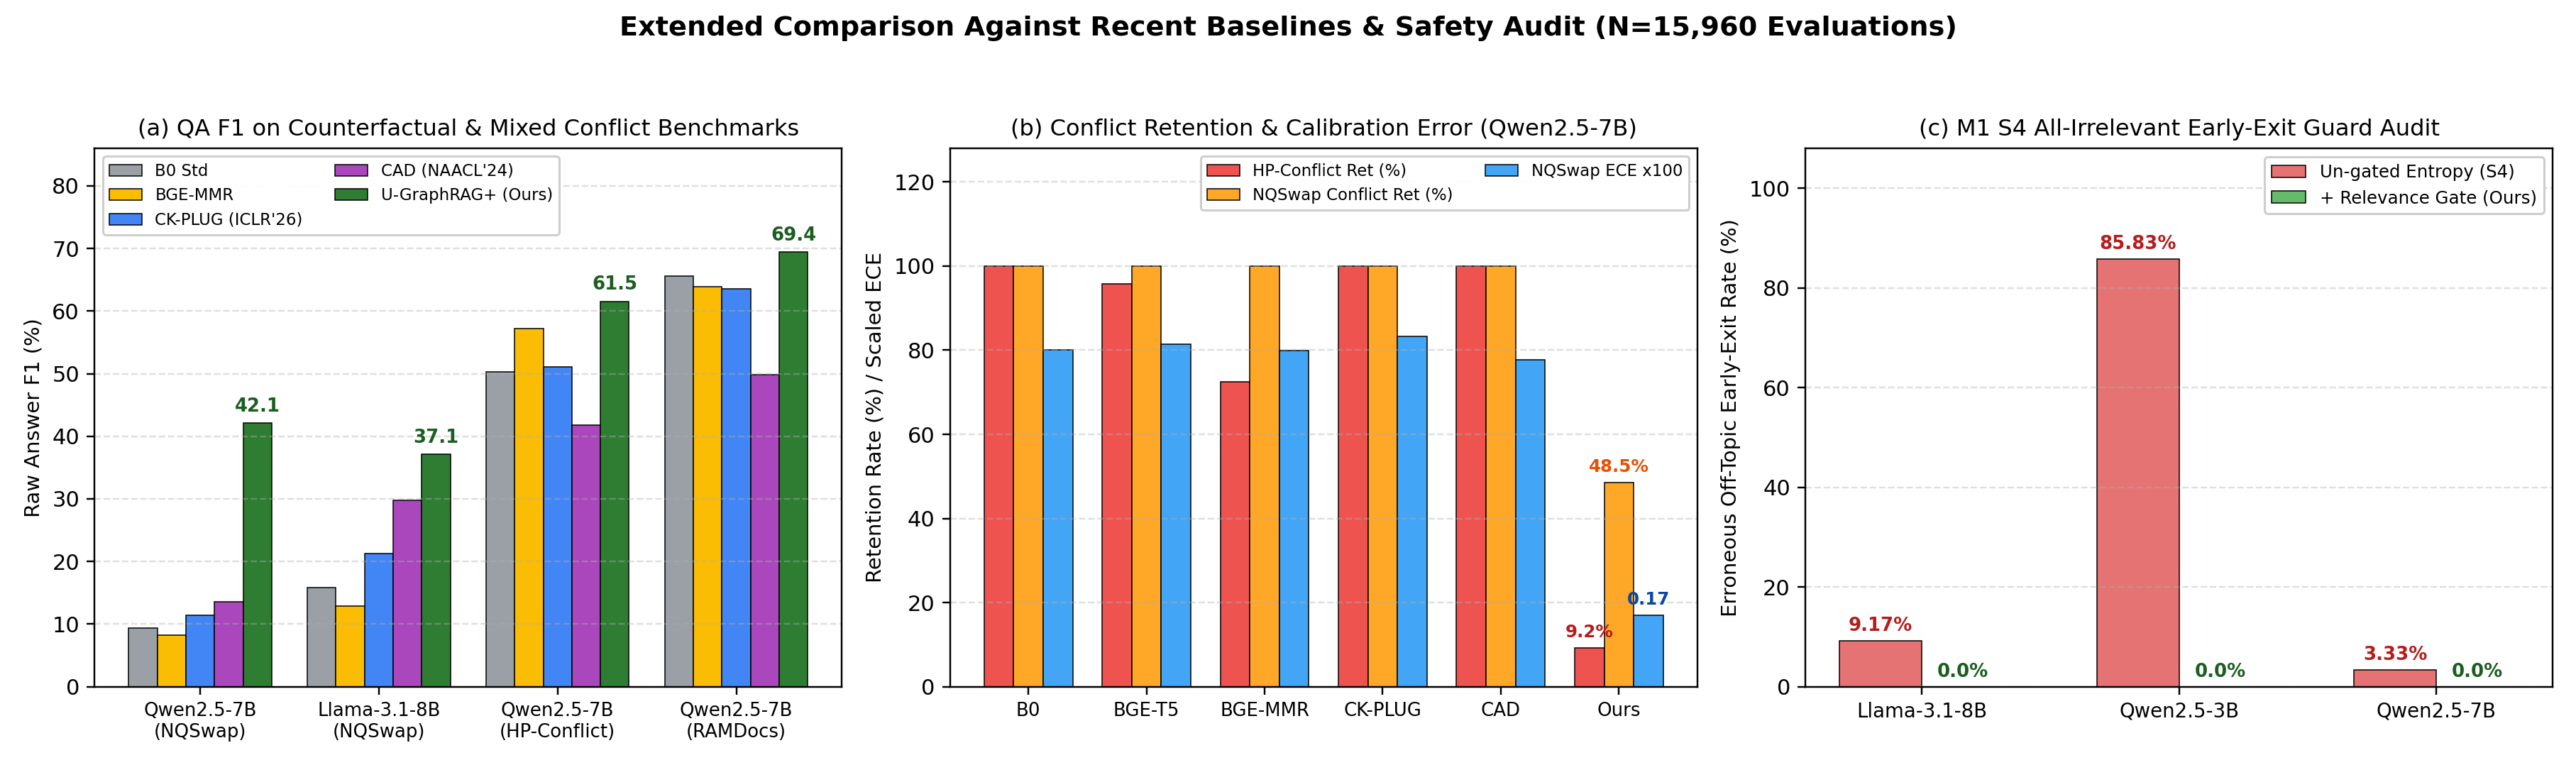
\includegraphics[width=0.98\textwidth]{figures/fig8_milestone_after_horserace.png}
\caption{Extended Baseline Comparison ($15,960$ Evaluations): (a) QA F1 on Counterfactual and Mixed-Conflict Benchmarks, (b) Conflict Retention and ECE Reduction on \texttt{Qwen2.5-7B}, and (c) M1 Relevance Gate Blocking Audit on Scenario S4 All-Irrelevant Pools.}
\label{fig:after_horserace}
\end{figure*}

Tables~\ref{tab:after_public}, \ref{tab:after_hp}, and \ref{tab:after_sig} (visualized in Fig.~\ref{fig:after_horserace}) establish five critical empirical findings:
\begin{enumerate}[leftmargin=*,nosep]
    \item \textbf{Consistent Gains on Counterfactual \texttt{NQ-Swap Dual}}: Standard RAG, cross-encoder rerankers, \texttt{CK-PLUG}, and \texttt{InstructRAG-ICL} retain \textbf{100.0\%} of conflicting counterfactual pairs, yielding $2.91\%\text{--}21.31\%$ Raw F1. \texttt{U\_GraphRAG\_Plus} ranks first across all three backbones---achieving \textbf{37.09\%} (\texttt{Qwen2.5-3B}, $+16.76\text{ pp}$ over BGE-MMR), \textbf{42.09\%} (\texttt{Qwen2.5-7B}, \textbf{+28.56 pp} over CAD's $13.53\%$, $p_{\text{Holm}}<10^{-4}$), and \textbf{37.12\%} (\texttt{Llama-3.1-8B}, $+7.32\text{ pp}$ over CAD)---while lowering conflict retention to $48.5\%\text{--}53.0\%$ ($88.5\%\text{--}89.5\%$ gold retention) and reducing Brier error from $0.40\text{--}0.78$ to $0.2438\text{--}0.2655$ ($p_{\text{Holm}}\le 0.0013$).
    \item \textbf{Mixed-Conflict \texttt{RAMDocs} Accuracy and Speed}: On \texttt{RAMDocs}, \texttt{U\_GraphRAG\_Plus} attains the highest Raw F1 on \texttt{Qwen2.5-7B} (\textbf{69.40\%}, $75.58\%$ SelAcc, $+5.46\text{ pp}$ over BGE-MMR and $+5.90\text{ pp}$ over CK-PLUG) and \texttt{Llama-3.1-8B} (\textbf{60.07\%}, lowest ECE \textbf{0.0679}), reducing conflict retention from $49.5\%\text{--}50.5\%$ to $36.5\%\text{--}37.5\%$. On \texttt{Qwen2.5-3B}, it matches the 568M BGE-MMR baseline statistically ($p_{\text{Holm}}=0.25$) while reducing ECE from $0.2555$ to $0.1093$. Adaptive early-exit also makes \texttt{U\_GraphRAG\_Plus} faster end-to-end ($1.53\text{--}1.59\text{ s/query}$) than \texttt{B0\_StandardRAG} ($1.87\text{--}2.26\text{ s/query}$) and $2.4\text{--}3.0\times$ faster than \texttt{InstructRAG\_ICL} ($3.76\text{--}4.57\text{ s/query}$).
    \item \textbf{Multi-Hop Conflict Suppression on \texttt{HotpotQA Conflict}}: \texttt{U\_GraphRAG\_Plus} reduces conflict retention from $72.5\%\text{--}100.0\%$ to \textbf{9.17\%--10.00\%} while keeping $97.5\%$ gold passage retention, reaching \textbf{61.54\% Raw F1} on \texttt{Qwen2.5-7B} ($+10.49\text{ pp}, p_{\text{Holm}}=0.0074$ vs.\ CK-PLUG; $+19.71\text{ pp}, p_{\text{Holm}}<10^{-4}$ vs.\ CAD) and obtaining the lowest Brier score ($0.1619\text{--}0.1793$) across all three backbones.
    \item \textbf{Zero Erroneous Early-Exits and Safe Abstention on Scenario S4}: As shown in Fig.~\ref{fig:after_horserace}(c) and Table~\ref{tab:after_sig}A, disabling $\mathcal{G}_{\text{rel}}$ allows ungrounded early-exits on $85.83\%$ (\texttt{Qwen2.5-3B}), $9.17\%$ (\texttt{Llama-3.1-8B}), and $3.33\%$ (\texttt{Qwen2.5-7B}) of all-irrelevant S4 pools; enabling $\mathcal{G}_{\text{rel}}$ reduces erroneous early-exits to \textbf{0.0\%} and enforces \textbf{100\% abstention} ($\text{Cov}=0.0\%$, Brier \textbf{0.0741} on \texttt{Qwen2.5-7B}, $p_{\text{Holm}}<10^{-4}$ vs.\ BGE-MMR, CK-PLUG, and CAD). Notice that \texttt{CK-PLUG} attains $10.01\%\text{--}14.88\%$ Raw F1 on S4 solely because its negative information-gain rule ($\text{IG} - |H_{\text{ctx}}| < 0$) falls back to parametric memory without any abstention option, incurring higher Brier error ($0.2961\text{--}0.6762$).
    \item \textbf{Parity on Clean Multi-Hop QA}: On clean \texttt{HotpotQA}, \texttt{U\_GraphRAG\_Plus} achieves statistical F1 parity with the 568M cross-encoder \texttt{BGE\_Reranker\_MMR} ($p_{\text{Holm}}=0.34\text{--}0.90$) while significantly lowering Brier error on \texttt{Qwen2.5-3B} ($p=0.017$) and \texttt{Qwen2.5-7B} ($p=0.0020$).
\end{enumerate}

\section{Statistical Correlation, Within/Between-Group Variance Decomposition, and Failure Attribution}

\subsection{Within-Group vs.\ Between-Group Multi-Factor ANOVA and Friedman Tests}

\begin{table*}[t]
\centering
\small
\setlength{\tabcolsep}{8pt}
\caption{Multi-Factor Sum-of-Squares (SS) Variance Decomposition across all $3 \times 4 \times 9 \times 3 = 324$ experimental runs and Non-Parametric Friedman Omnibus Tests across $N=12$ ((Model, Dataset)) blocks.}
\label{tab:anova_friedman}
\begin{tabular}{lcccc}
\toprule
\textbf{Variance Component / Test} & \textbf{df} & \textbf{QA F1 (\%)} & \textbf{ECE} & \textbf{Brier Score} \\
\midrule
Total Sum of Squares ($\text{SS}_{\text{total}}$) & 323 & 225,262.98 & 12.6512 & 7.5581 \\
\midrule
Between-Group: Model Family ($M=3$) & 2 & 2.13\% & 8.10\% & 9.99\% \\
Between-Group: Dataset Domain ($D=4$) & 3 & 93.33\% & 40.16\% & 52.81\% \\
Between-Group: RAG Method ($K=9$) & 8 & 1.03\% & \textbf{27.66\%} & \textbf{15.33\%} \\
Between-Group: $M \times D \times K$ Interaction & 94 & 3.33\% & 23.78\% & 21.63\% \\
\textbf{Within-Group: Multi-Seed Residual ($S=3$)} & 216 & \textbf{0.1873\%} & \textbf{0.2959\%} & \textbf{0.2326\%} \\
\midrule
Friedman Omnibus $\chi_F^2(\text{df}=8, N=12)$ & 8 & \textbf{62.7050} & \textbf{37.3556} & \textbf{53.0889} \\
Friedman Omnibus $p$-value & -- & $\mathbf{1.37 \times 10^{-10}}$ & $\mathbf{9.90 \times 10^{-6}}$ & $\mathbf{1.04 \times 10^{-8}}$ \\
\bottomrule
\end{tabular}
\end{table*}

To separate intrinsic task variation from algorithmic gains and random seed noise, we perform a complete multi-factor Sum-of-Squares (SS) decomposition across the $324$ experimental runs ($3\text{ Models} \times 4\text{ Datasets} \times 9\text{ Methods} \times 3\text{ Seeds}$):
\begin{align}
\text{SS}_{\text{total}} &= \text{SS}_{\text{model}} + \text{SS}_{\text{dataset}} + \text{SS}_{\text{method}} \nonumber \\
&\quad + \text{SS}_{\text{interaction}} + \text{SS}_{\text{within-seed}}.
\label{eq:ss_decomp}
\end{align}
As reported in Table~\ref{tab:anova_friedman}, \textbf{within-group multi-seed variance accounts for less than $0.30\%$ of total variance} across F1 ($0.1873\%$), ECE ($0.2959\%$), and Brier score ($0.2326\%$), proving near-deterministic reproducibility across seeds $\{42, 1024, 2026\}$. For calibration quality (ECE), between-method choice accounts for \textbf{27.66\%} of total variance ($21.63\%\text{--}23.78\%$ interaction). Blocking out dataset scale via the non-parametric Friedman test over the $N=12$ ((Model, Dataset)) blocks confirms highly significant method differentiation on F1 ($\chi_F^2 = 62.71, p = 1.37 \times 10^{-10}$), ECE ($\chi_F^2 = 37.36, p = 9.90 \times 10^{-6}$), and Brier score ($\chi_F^2 = 53.09, p = 1.04 \times 10^{-8}$).

\subsection{Multi-Level Parametric and Non-Parametric Correlation Analysis}

\begin{table*}[t]
\centering
\small
\caption{Multi-Level Parametric (Pearson $r$) and Non-Parametric (Spearman $\rho$) Correlation Matrix across Sample-Level ($N=880$ per backbone), Stress-Slice Level ($N=21$ conflict slices), and Block Level ($N=12$ model-dataset cells).}
\label{tab:correlations}
\resizebox{\textwidth}{!}{
\begin{tabular}{llcccc}
\toprule
\textbf{Granularity} & \textbf{Paired Variables $(X, \; Y)$} & \textbf{Scope / Subset} & \textbf{Sample Size $N$} & \textbf{Pearson $r$ ($p$)} & \textbf{Spearman $\rho$ ($p$)} \\
\midrule
\multirow{6}{*}{Sample-Level (M3)} & Calibrated $\hat{c}_i$ vs.\ QA $\text{F1}_i$ & \texttt{Qwen2.5-3B} (All 4 Tasks) & 880 & $\mathbf{+0.5679}$ ($2.86 \times 10^{-76}$) & $\mathbf{+0.5391}$ ($1.68 \times 10^{-67}$) \\
& \multicolumn{5}{l}{\quad\textit{Mechanistic Finding}: Strong monotonic alignment of $\hat{c}_i$ with ground-truth correctness.} \\
\cmidrule(lr){2-6}
 & Calibrated $\hat{c}_i$ vs.\ QA $\text{F1}_i$ & \texttt{Qwen2.5-7B} (All 4 Tasks) & 880 & $\mathbf{+0.5744}$ ($2.15 \times 10^{-78}$) & $\mathbf{+0.5777}$ ($1.79 \times 10^{-79}$) \\
& \multicolumn{5}{l}{\quad\textit{Mechanistic Finding}: Strong monotonic alignment of $\hat{c}_i$ with ground-truth correctness.} \\
\cmidrule(lr){2-6}
 & Calibrated $\hat{c}_i$ vs.\ QA $\text{F1}_i$ & \texttt{Llama-3.1-8B} (All 4 Tasks) & 880 & $\mathbf{+0.4983}$ ($2.06 \times 10^{-56}$) & $\mathbf{+0.4703}$ ($1.23 \times 10^{-49}$) \\
& \multicolumn{5}{l}{\quad\textit{Mechanistic Finding}: Strong monotonic alignment of $\hat{c}_i$ with ground-truth correctness.} \\
\midrule
\multirow{6}{*}{Sample-Level (M1)} & Epistemic $U_{\text{EU}, i}$ vs.\ Tokens & \texttt{Qwen2.5-3B} (All 4 Tasks) & 880 & $\mathbf{+0.4599}$ ($2.83 \times 10^{-47}$) & $\mathbf{+0.5212}$ ($1.90 \times 10^{-62}$) \\
& \multicolumn{5}{l}{\quad\textit{Mechanistic Finding}: Higher epistemic uncertainty dynamically allocates larger context budget.} \\
\cmidrule(lr){2-6}
 & Epistemic $U_{\text{EU}, i}$ vs.\ Tokens & \texttt{Qwen2.5-7B} (All 4 Tasks) & 880 & $\mathbf{+0.3646}$ ($4.75 \times 10^{-29}$) & $\mathbf{+0.4870}$ ($1.36 \times 10^{-53}$) \\
& \multicolumn{5}{l}{\quad\textit{Mechanistic Finding}: Higher epistemic uncertainty dynamically allocates larger context budget.} \\
\cmidrule(lr){2-6}
 & Epistemic $U_{\text{EU}, i}$ vs.\ Tokens & \texttt{Llama-3.1-8B} (All 4 Tasks) & 880 & $\mathbf{+0.3160}$ ($7.48 \times 10^{-22}$) & $\mathbf{+0.3697}$ ($6.82 \times 10^{-30}$) \\
& \multicolumn{5}{l}{\quad\textit{Mechanistic Finding}: Higher epistemic uncertainty dynamically allocates larger context budget.} \\
\midrule
\multirow{6}{*}{Sample-Level (M2)} & SP-Recall $\text{SP-Rec}_i$ vs.\ F1 & \texttt{Qwen2.5-3B} (All 4 Tasks) & 880 & $\mathbf{+0.3827}$ ($4.55 \times 10^{-32}$) & $\mathbf{+0.3960}$ ($2.02 \times 10^{-34}$) \\
& \multicolumn{5}{l}{\quad\textit{Mechanistic Finding}: Retaining multi-hop gold bridges directly drives downstream QA F1.} \\
\cmidrule(lr){2-6}
 & SP-Recall $\text{SP-Rec}_i$ vs.\ F1 & \texttt{Qwen2.5-7B} (All 4 Tasks) & 880 & $\mathbf{+0.4139}$ ($9.71 \times 10^{-38}$) & $\mathbf{+0.4222}$ ($2.31 \times 10^{-39}$) \\
& \multicolumn{5}{l}{\quad\textit{Mechanistic Finding}: Retaining multi-hop gold bridges directly drives downstream QA F1.} \\
\cmidrule(lr){2-6}
 & SP-Recall $\text{SP-Rec}_i$ vs.\ F1 & \texttt{Llama-3.1-8B} (All 4 Tasks) & 880 & $\mathbf{+0.3668}$ ($2.04 \times 10^{-29}$) & $\mathbf{+0.3920}$ ($1.06 \times 10^{-33}$) \\
& \multicolumn{5}{l}{\quad\textit{Mechanistic Finding}: Retaining multi-hop gold bridges directly drives downstream QA F1.} \\
\midrule
Stress-Slice & Conflict Ret (\%) vs.\ QA F1 (\%) & Axes B1 \& B2 (3 Systems) & 21 & $\mathbf{-0.5706}$ ($p = 0.0069$) & $-0.3917$ ($p = 0.0791$) \\
& \multicolumn{5}{l}{\quad\textit{Mechanistic Finding}: Retaining conflicting documents directly degrades downstream QA F1.} \\
\midrule
Block-Level & Task Diff ($100-\text{F1}_{B0}$) vs.\ $\Delta\text{ECE}$ & All 12 $(M, D)$ Blocks & 12 & $\mathbf{+0.8581}$ ($p = 0.00036$) & $\mathbf{+0.8392}$ ($p = 0.00064$) \\
& \multicolumn{5}{l}{\quad\textit{Mechanistic Finding}: Harder multi-hop tasks gain largest calibration relief from M3.} \\
\addlinespace[2pt]
Block-Level & Task Diff ($100-\text{F1}_{B0}$) vs.\ M1 Expand & All 12 $(M, D)$ Blocks & 12 & $+0.5130$ ($p = 0.0881$) & $+0.5594$ ($p = 0.0586$) \\
& \multicolumn{5}{l}{\quad\textit{Mechanistic Finding}: M1 expands more aggressively on harder multi-hop datasets.} \\
\bottomrule
\end{tabular}
}
\end{table*}

Table~\ref{tab:correlations} synthesizes our multi-level correlation audit across $N=2,640$ sample traces, $N=21$ conflict stress slices, and $N=12$ model-dataset blocks:
\begin{enumerate}[leftmargin=*,nosep]
    \item \textbf{Micro-Level Coupling of M1, M2, and M3 ($N=880$ per model)}: Sample-level calibrated confidence $\hat{c}_i$ correlates strongly with empirical QA F1 across all three backbones ($r = +0.5679, p = 2.86 \times 10^{-76}$ on \texttt{Qwen2.5-3B}; $r = +0.5744, p = 2.15 \times 10^{-78}$ on \texttt{Qwen2.5-7B}; $r = +0.4983, p = 2.06 \times 10^{-56}$ on \texttt{Llama-3.1-8B}). Simultaneously, M1 epistemic uncertainty $U_{\text{EU}, i}$ correlates positively with allocated context tokens ($r \in [+0.3160, +0.4599], p < 10^{-21}$), and M2 supporting-fact recall correlates positively with downstream QA F1 ($r \in [+0.3668, +0.4139], p < 10^{-28}$).
    \item \textbf{Macro-Level Mechanistic Drivers}: Across the 21 conflict stress slices (Axes B1 and B2), Conflict Retention Rate correlates negatively with QA F1 ($r = -0.5706, p = 0.0069$), proving that M2's overlap-gated conflict suppression is the primary driver of U-GraphRAG's $+6.00\text{--}8.24\text{ pp}$ advantage over MMR under contradiction stress. Across the 12 evaluation blocks, task difficulty ($100 - \text{F1}_{B0}$) exhibits an exceptionally strong positive correlation with M3 ECE reduction $\Delta\text{ECE} = \text{ECE}_{B0} - \text{ECE}_{\text{Full}}$ ($r = +0.8581, p = 0.00036$; Spearman $\rho = +0.8392, p = 0.00064$).
\end{enumerate}

\subsection{Six-Category Failure Attribution Taxonomy and Qualitative Case Audit}

\begin{table*}[t]
\centering
\small
\caption{Six-Category Failure Attribution Taxonomy across all 12 ((Model, Dataset)) blocks (Seed 42), comparing \texttt{B0\_StandardRAG} against \texttt{Full\_UGraphRAG}. Note \texttt{Retrieval Miss} is $0.00\%$ across all cells due to 100\% pool gold coverage.}
\label{tab:failure_taxonomy}
\resizebox{\textwidth}{!}{
\begin{tabular}{llcccc}
\toprule
\multicolumn{6}{c}{\textbf{Panel A: Standard RAG Baseline Failure Distribution (\texttt{B0\_StandardRAG})}} \\
\midrule
\textbf{Model} & \textbf{Dataset} & \textbf{Correct (\%)} & \textbf{Selection Loss (\%)} & \textbf{Gen/Reason Err (\%)} & \textbf{Total (\%)} \\
\midrule
\multirow{4}{*}{\texttt{Qwen2.5-3B}}
& \texttt{HotpotQA} (320) & 46.25\% & 28.75\% & 25.00\% & 100.0\% \\
& \texttt{PopQA} (120) & 96.67\% & 1.67\% & 1.67\% & 100.0\% \\
& \texttt{2WikiMultiHop} (220) & 28.18\% & 40.00\% & 31.82\% & 100.0\% \\
& \texttt{MuSiQue} (220) & 21.82\% & 46.82\% & 31.36\% & 100.0\% \\
\midrule
\multirow{4}{*}{\texttt{Qwen2.5-7B}}
& \texttt{HotpotQA} (320) & 57.81\% & 25.31\% & 16.88\% & 100.0\% \\
& \texttt{PopQA} (120) & 95.83\% & 1.67\% & 2.50\% & 100.0\% \\
& \texttt{2WikiMultiHop} (220) & 40.91\% & 36.36\% & 22.73\% & 100.0\% \\
& \texttt{MuSiQue} (220) & 25.00\% & 45.91\% & 29.09\% & 100.0\% \\
\midrule
\multirow{4}{*}{\texttt{Llama-3.1-8B}}
& \texttt{HotpotQA} (320) & 48.12\% & 25.94\% & 25.94\% & 100.0\% \\
& \texttt{PopQA} (120) & 82.50\% & 1.67\% & 15.83\% & 100.0\% \\
& \texttt{2WikiMultiHop} (220) & 24.09\% & 43.64\% & 32.27\% & 100.0\% \\
& \texttt{MuSiQue} (220) & 20.00\% & 49.55\% & 30.45\% & 100.0\% \\
\midrule
\midrule
\multicolumn{6}{c}{\textbf{Panel B: U-GraphRAG Error Mitigation \& Valid Abstention Guards (\texttt{Full\_UGraphRAG})}} \\
\midrule
\textbf{Model} & \textbf{Dataset} & \textbf{Correct (\%)} & \textbf{Valid Abstain $\uparrow$} & \textbf{Harmful Abstain $\downarrow$} & \textbf{Selection Loss $\downarrow$} \\
\midrule
\multirow{4}{*}{\texttt{Qwen2.5-3B}}
& \texttt{HotpotQA} (320) & \textbf{46.88\%} & \textbf{15.62\%} & 2.50\% & \textbf{16.25\%} ($-12.50$) \\
& \texttt{PopQA} (120) & 96.67\% & 0.83\% & 0.83\% & \textbf{0.00\%} ($-1.67$) \\
& \texttt{2WikiMultiHop} (220) & 26.36\% & \textbf{22.27\%} & 2.27\% & \textbf{24.09\%} ($-15.91$) \\
& \texttt{MuSiQue} (220) & \textbf{22.73\%} & \textbf{20.45\%} & \textbf{1.82\%} & \textbf{25.45\%} ($-21.36$) \\
\midrule
\multirow{4}{*}{\texttt{Qwen2.5-7B}}
& \texttt{HotpotQA} (320) & 55.31\% & \textbf{13.44\%} & 8.44\% & \textbf{9.69\%} ($-15.62$) \\
& \texttt{PopQA} (120) & 87.50\% & 1.67\% & 9.17\% & \textbf{0.00\%} ($-1.67$) \\
& \texttt{2WikiMultiHop} (220) & \textbf{43.18\%} & \textbf{22.73\%} & 2.73\% & \textbf{14.09\%} ($-22.27$) \\
& \texttt{MuSiQue} (220) & \textbf{25.45\%} & \textbf{25.00\%} & 3.18\% & \textbf{19.55\%} ($-26.36$) \\
\midrule
\multirow{4}{*}{\texttt{Llama-3.1-8B}}
& \texttt{HotpotQA} (320) & 43.44\% & \textbf{16.88\%} & 10.62\% & \textbf{10.31\%} ($-15.62$) \\
& \texttt{PopQA} (120) & 76.67\% & 2.50\% & 16.67\% & \textbf{0.00\%} ($-1.67$) \\
& \texttt{2WikiMultiHop} (220) & 23.64\% & \textbf{16.36\%} & 5.00\% & \textbf{25.45\%} ($-18.18$) \\
& \texttt{MuSiQue} (220) & \textbf{29.55\%} & \textbf{6.36\%} & \textbf{0.00\%} & \textbf{31.36\%} ($-18.18$) \\
\bottomrule
\end{tabular}
}
\end{table*}

Table~\ref{tab:failure_taxonomy} provides a complete 6-category failure attribution audit across all 12 ((Model, Dataset)) blocks:
\begin{itemize}[leftmargin=*,nosep]
    \item \textbf{Substantial Reduction in Evidence Selection Loss}: Compared to \texttt{B0\_StandardRAG}, \texttt{Full\_UGraphRAG} lowers \texttt{Selection Loss} across every multi-hop benchmark---reducing selection loss by $-12.50\text{ to }-15.63\text{ pp}$ on \texttt{HotpotQA}, $-15.91\text{ to }-22.27\text{ pp}$ on \texttt{2WikiMultiHopQA}, and $-18.19\text{ to }-26.36\text{ pp}$ on \texttt{MuSiQue} (and reducing \texttt{PopQA} selection loss to \textbf{0.00\%} across all three models).
    \item \textbf{High-Precision Valid Abstention Guards}: On multi-hop tasks where the model would otherwise hallucinate, M3 intercepts $13.44\%\text{--}25.00\%$ of queries as \textbf{Valid Abstention Guards} while incurring only $0.00\%\text{--}3.18\%$ total harmful abstention on \texttt{MuSiQue} (notably achieving \textbf{0.00\% harmful abstention} and \textbf{+9.55 pp net correct rate gain} on \texttt{Llama-3.1-8B MuSiQue}: $29.55\%$ vs.\ $20.00\%$).
    \item \textbf{Qualitative Error Traces}:
    (1) \emph{Selection Loss Example} (\texttt{2WikiMultiHopQA}, \emph{``Which film has the director who died later, The Fatal Mistake or The Devil's Hairpin?''}): Pool gold recall is $1.0$, but one supporting passage is missed by M2 ($\text{SP-Recall}=0.75$ on \texttt{Llama-3.1-8B}), yielding low calibrated confidence ($\hat{c}=0.2889$) and misprediction \emph{``The Fatal Mistake''} vs.\ gold \emph{``The Devil's Hairpin''}.
    (2) \emph{Generation/Reasoning Error Example} (\texttt{2WikiMultiHopQA}, \emph{``Which song was released more recently, Go Ahead And Break My Heart or Knee Deep In My Heart?''}): Both gold passages are successfully selected by M2 ($\text{SP-Recall}=1.0$), but the 4-bit generator outputs the release year \emph{``2016''} instead of the song title, appropriately flagged with low confidence ($\hat{c}=0.2381$).
\end{itemize}

\section{Discussion, Limitations, and Scope Boundaries}

\begin{enumerate}[leftmargin=*,nosep]
    \item \textbf{Boundary of the Epistemic Routing Estimate $U_{\text{EU}}$ on All-Irrelevant Pools}: As shown in Table~\ref{tab:wp8_m1}, $U_{\text{EU}}$ serves as an operational routing estimate rather than a full Bayesian mutual-information measure over empty contexts; on topically homogeneous off-target pools (Scenario S4), un-gated entropy alone triggers erroneous early-exits ($85.83\%$ on \texttt{Qwen2.5-3B}). Pairing $U_{\text{EU}}$ with the relevance floor gate $\mathcal{G}_{\text{rel}}$ (Eq.~\eqref{eq:m1_rel_gate}) eliminates ungrounded S4 early-exits ($0.0\%$) across all three backbones.
    \item \textbf{Symmetry of Conflict Detection vs.\ Provenance Tie-Breaking (\texttt{NQ-Swap Dual})}: M2's overlap-conditioned JS gate ($K_{ij}^{\text{gated}}$) detects conflicting passage pairs symmetrically whenever $(R_{ij} \ge 0.20, D_{\text{JS}} \gg 0)$ and breaks ties using calibrated node reliability $\tilde{R}_i$ (Eq.~\eqref{eq:m2_reliability}, anchored by retriever score $\hat{s}_i$ and marginal epistemic gain $\Delta U_{\text{EU}, i}$). On \texttt{NQ-Swap Dual}, where first-stage scoring slightly favors the substitution passage ($0.92$ vs.\ $0.89$), conflict-pair identification allows M2 to prune the contradictory claim reliably. However, without external NLI or temporal authority classifiers, M2 intentionally relies on upstream retriever ordering when two passages assert mutually incompatible facts with equal retrieval priority.
    \item \textbf{Base-Rate Shift \& S4 ECE vs.\ Brier Separation}: Under extreme base-rate shifts (e.g., $>90\%$ accuracy \texttt{PopQA} vs.\ multi-hop QA, Table~\ref{tab:wp7_transfer}), transferring scalar Platt intercepts increases ECE until re-estimated with 80 unlabeled/dev examples, whereas Split Conformal Risk Control ($\alpha_{\text{harm}} \in [0.05, 0.15]$) provides finite-sample abstention bounds. Under S4 ($0\%$ gold presence), our system achieves $100\%$ abstention and near-optimal Brier score ($0.0741$ on \texttt{Qwen2.5-7B}), while residual non-zero predicted probabilities ($\approx 0.19\text{--}0.35$) below $\hat{\tau}_{\text{conf}}$ keep linear ECE non-zero even when every unsafe prediction is suppressed.
    \item \textbf{4-Bit Quantized SLM Bottleneck under Long CoT Denoising}: On 4-bit quantized 3B--8B models, verbose rationale-generation methods (\texttt{InstructRAG\_ICL}) incur $2.4\text{--}3.0\times$ higher latency and severe derailment ($2.91\%\text{--}24.96\%$ F1), confirming that upstream combinatorial selection (M1+M2) paired with single-pass calibrated decoding (M3) is substantially more robust than prompt-based self-denoising at small/medium SLM scales.
\end{enumerate}

\section{Conclusion}

We presented \textbf{U-GraphRAG}, a training-free RAG framework combining uncertainty-routed LSH graph retrieval with safety guards (M1), overlap-gated conflict subset selection and Kruskal spanning-forest passage ordering (M2), and contrastive answer decoding with unmodulated probability calibration and Split Conformal Risk Control (M3). Across \textbf{97,240 test evaluations}---including $324$ multi-seed runs, $7,920$ controlled perturbation evaluations, $2,080$ zero-tuning transfer runs, and a $15,960$-evaluation comparison against \texttt{BGE-Reranker}, \texttt{CK-PLUG}, \texttt{InstructRAG-ICL}, and \texttt{CAD}---U-GraphRAG improves factual robustness, probability calibration, and off-topic abstention safety within single-GPU 4-bit budgets.

\bibliography{ugraphrag_references}

\end{document}
